\documentclass[11pt]{report}
\usepackage{graphicx}
\usepackage{amsmath, amssymb}
%\usepackage{fleqn} %sets equation to left
\usepackage{fancyhdr}
\usepackage[usenames,dvipsnames]{color}
\usepackage{xcolor}
\usepackage{multido}
\usepackage{vmargin}
%\usepackage{floatflt}
\usepackage{subfigure}
\usepackage{epsfig}
\usepackage{tabularx}
\usepackage{xr} % for cross reference to external documents
\usepackage{alltt}
\usepackage{url}
\usepackage{pstricks,pst-node,pst-tree,pst-plot}
\usepackage{listings}
% Figure and table caption in italic fonts
\makeatletter
\renewcommand{\fnum@figure}[1]{\small \textit{\figurename~\thefigure}: \it }
\renewcommand{\fnum@table}[1]{\small \textit{\tablename~\thetable}: \it }
\makeatother
% Fuzz -------------------------------------------------------------------
\hfuzz4pt % Don't bother to report over-full boxes if over-edge is < 2pt
\vfuzz=\hfuzz
% THEOREM Environments ---------------------------------------------------
\newtheorem{theorem}{Theorem}[section]
\newtheorem{definition}[theorem]{Definition}
\newtheorem{lemma}[theorem]{Lemma}
\newtheorem{corollary}[theorem]{Corollary}
\newtheorem{proposition}[theorem]{Proposition}
\newtheorem{example}[theorem]{Example}
\newtheorem{remark}[theorem]{Remark}
\newtheorem{algorithm}[theorem]{Algorithm}
\newtheorem{assumption}[theorem]{Assumption}


% \renewcommand{\epsilon}{{\red \varepsilon}}
% \renewcommand{\cdot}{{\red \bullet}}
% List for code description ---------------------------------------------
% MWetter@lbl.gov
\makeatletter
\newenvironment{codedescription}
               {\list{}{\labelwidth\z@ \itemindent-\leftmargin
                        \let\makelabel\codedescriptionlabel}}
               {\endlist}
\newcommand*\codedescriptionlabel[1]{\hspace\labelsep
                                \hspace{1em}\normalfont\ttfamily#1}

% Section formats ------------------------------- --------------------
% MWetter@lbl.gov
\renewcommand{\chapter}{\@startsection
  {chapter}%                          % the name
  {0}%                                % the level
  {0mm}%                            % the indent
  {2\baselineskip}%                   % the beforeskip
  {\baselineskip}%                 % the afterskip
%  {\normalfont\fontfamily{phv}\fontseries{b}\fontsize{9}{11}\selectfont}}%  % the style
  {\pagebreak \normalfont\sffamily\huge\bfseries \raggedright}}%  % the style

\renewcommand{\section}{\@startsection
  {section}%                          % the name
  {1}%                                % the level
  {0mm}%                            % the indent
  {\baselineskip}%                   % the beforeskip
  {\baselineskip}%                 % the afterskip
  {\normalfont\sffamily\Large\bfseries \raggedright}}%  % the style

\renewcommand{\subsection}{\@startsection
  {subsection}%                          % the name
  {2}%                                % the level
  {0mm}%                            % the indent
  {\baselineskip}%                   % the beforeskip
  {0.5\baselineskip}%                 % the afterskip
  {\normalfont\sffamily\large\bfseries \raggedright}}%  % the style

\renewcommand{\subsubsection}{\@startsection
  {subsubsection}%                          % the name
  {3}%                                % the level
  {0mm}%                            % the indent
  {\baselineskip}%                   % the beforeskip
  {0.5\baselineskip}%                 % the afterskip
  {\normalfont\sffamily\bfseries \raggedright}}%  % the style

\makeatother
% end of list ---------------------------------------------

\newcommand{\clarify}[1]{\colorbox{yellow}{ #1 }}

\newcommand{\lab}[1]{\label{#1} \hfill \mbox{\tiny {\tt [#1]}}}
%%%%%%%%%%%%%%%%%%%%%%%%%%%%%%%%%%%%%%%%%%%%%%%%%%%%%
% Remove comment of next line for the final print out
%%%%%%%%%%%%%%%%%%%%%%%%%%%%%%%%%%%%%%%%%%%%%%%%%%%%%
\renewcommand{\lab}[1]{\label{#1}}


% Page layout -------------------------------------------------------------
%\setlength{\textwidth}{14cm} 
\pagestyle{fancy}
\setlength{\textwidth}{12cm} 
\setlength{\textheight}{20cm}
\setlength{\headheight}{35mm}
\setlength{\headwidth}{\textwidth}
\setlength{\headsep}{5mm}
\setlength{\oddsidemargin}{3.7cm}
\setlength{\evensidemargin}{\oddsidemargin}
% next lines from 'The LaTeX Companion', Sec. 4.3
\addtolength{\headwidth}{\marginparsep}
\addtolength{\headwidth}{\marginparwidth}

% -------------------------------------------------------------------
% Code formatting
\lstset{ %
language=Java,                % the language of the code
stringstyle=\ttfamily,
basicstyle=\footnotesize,       % the size of the fonts that are used for the code
%numbers=left,                   % where to put the line-numbers
numberstyle=\footnotesize,      % the size of the fonts that are used for the line-numbers
%stepnumber=2,                   % the step between two line-numbers. If it's 1, each line 
                                % will be numbered
commentstyle=\color{ForestGreen},
numbersep=5pt,                  % how far the line-numbers are from the code
backgroundcolor=\color{gray!10},  % choose the background color. You must add \usepackage{color}
showspaces=false,               % show spaces adding particular underscores
showstringspaces=false,         % underline spaces within strings
showtabs=false,                 % show tabs within strings adding particular underscores
tabsize=2,                      % sets default tabsize to 2 spaces
captionpos=b,                   % sets the caption-position to bottom
breaklines=false,                % sets automatic line breaking
linewidth=\headwidth,
breakatwhitespace=false,        % sets if automatic breaks should only happen at whitespace
title=\lstname,                 % show the filename of files included with \lstinputlisting;
                                % also try caption instead of title
escapeinside={\%*}{*)},         % if you want to add a comment within your code
morekeywords={*,...}            % if you want to add more keywords to the set
}
% Depth of table of contents -----------------------------------------
\setcounter{tocdepth}{4}


% PDF Links --------------------------------------------------------
\usepackage[ps2pdf,colorlinks]{hyperref}
  \hypersetup{backref, %
    colorlinks=true, %
    linkcolor=black, %
    anchorcolor=black, %
    citecolor=black, %
    filecolor=black, % Color for URLs which open local files. 
    menucolor=black, % Color for Acrobat menu items.
    pagecolor=black, % Color for links to other pages. 
    urlcolor=black, %
    pdftitle={GenOpt manual}, %
    pdfauthor={Michael Wetter}, %
    pdfsubject={}, %
    pdfkeywords={}%
  }

% commands for mathematical description ------------------------------
\renewcommand{\Re}{{\mathbb R}}
\newcommand{\Rep}{{\Re_{+}}}
\newcommand{\Na}{{\mathbb N}}
\newcommand{\Z}{{\mathbb Z}}
\newcommand{\Co}{{\mathbb C}}

\newcommand{\codi}[2]{{\mathcal{C}^{#1}(#2)}}

\newcommand{\depd}{(\cdot)}
\newcommand{\depdd}{(\cdot, \cdot)}
\newcommand{\depddd}{(\cdot, \cdot, \cdot)}
\newcommand{\depdddd}{(\cdot, \cdot, \cdot, \cdot)}
\newcommand{\RR}{\Re \times \Re}
\newcommand{\RRR}{\Re \times \Re \times \Re}

\newcommand{\vect}[1]{\mathtt{vect}\left( #1 \right) }
\newcommand{\vectp}[1]{\mathop{\mathtt{vect}}_{p}\left( #1 \right) }
\newcommand{\vectcwwi}[1]{\mathop{\mathtt{vect}}_{i, \, i \neq p, \, j}\left( #1 \right) }
\newcommand{\diag}[1]{\mathtt{diag}\left( #1 \right) }
\newcommand{\argmin}{\mathop{\arg \min}}
\newcommand{\argmax}{\mathop{\arg \max}}

\hyphenation{Torczon}

%QED box, from the TeXbook, p. 106. ----------------------------------
%\newcommand\qed{{\unskip\nobreak\hfil\penalty50\hskip2em\vadjust{}
%    \nobreak\hfil$\Box$\parfillskip=0pt\finalhyphendemerits=0\par}}
\newcommand{\rbox}{{ \hfill \framebox{} }}
% Depth of section numbering and table of contents -------------------
\setcounter{secnumdepth}{5}
\setcounter{tocdepth}{4}
\renewcommand{\thesubsubsection}{\alph{subsubsection})}
\renewcommand{\theparagraph}{(\roman{paragraph})}

% commands for physical description ----------------------------------

\newcommand{\depx}{(x)}

% Line spacing -----------------------------------------------------------
\newlength{\defbaselineskip}
\setlength{\defbaselineskip}{\baselineskip}
%\newcommand{\setlinespacing}[1]%
%           {\setlength{\baselineskip}{#1 \defbaselineskip}}
\newcommand{\doublespacing}{\setlength{\baselineskip}
                           {2.0 \defbaselineskip}}
\newcommand{\singlespacing}{\setlength{\baselineskip}{\defbaselineskip}}
\newcommand{\onehalfspacing}{\setlength{\baselineskip}
                           {1.5 \defbaselineskip}}

\newcommand{\codeem}[1]{{\fontfamily{pcr}\fontseries{b}\fontsize{10}{12}\selectfont #1}}

%\newcommand{\genoptversion}{3.0.0\@$\beta$2\@ }
\newcommand{\genoptversion}{3.1.0\@ }
\newcommand{\javaversion}{2 v1.6.0\@ }
\renewcommand{\date}{December 8, 2011\@}
%%\renewcommand{\date}{\today}
\newcommand{\copyrightyears}{1998-2011}
% Headings ---------------------------------------------------------------
% right header entry
\lhead{GenOpt\\Generic Optimization Program\\Version \genoptversion}
\rhead{Lawrence Berkeley National Laboratory\\Building Technologies Department\\Simulation Research Group}
\lfoot{\tiny{Copyright (c) \copyrightyears\\The Regents of the University of California (through Lawrence Berkeley National Laboratory),\\subject to receipt of any required approvals from U.S. Department of Energy. All rights reserved.}}
\cfoot{}
\rfoot{\thepage}
% line at header and footer
\renewcommand{\headrulewidth}{1pt}
\renewcommand{\footrulewidth}{1pt}

% select Helvetica as default roman font --------------------------------
\renewcommand\sfdefault{phv}

% external documents, for cross reference --------------------------------
\externaldocument{introduction}
\externaldocument{problems}
\externaldocument{summary}
\externaldocument{algGPS}
\externaldocument{algDisArmGra}
\externaldocument{algParSwaOpt}
\externaldocument{algGPSPSO}
% no longer part of GenOpt since 3.0.0 \externaldocument{algHooJee}
\externaldocument{algSimplex}
\externaldocument{algOneDim}
\externaldocument{algParametric}
\externaldocument{constraints}
\externaldocument{program}
\externaldocument{install}
\externaldocument{problemsetup}
\externaldocument{end}
\externaldocument{appendix}
% Begin of document -------------------------------------------------------
\begin{document}
% Contents ----------------------------------------------------------------
\begin{titlepage}
\begin{minipage}{\headwidth}
\rput[l](0,2){
\includegraphics[scale=0.5]{img/lbl_text.eps}}
\vspace{-1cm}
\begin{flushright}
%%\large{Technical Report LBNL-2077E}
\large{~}
\\[5mm]
\hrulefill
\\[5mm]
 \Large\sffamily\bfseries{GenOpt}$^{\mathsf{(R)}}$\\
 \Large\sffamily\bfseries{Generic Optimization Program}\\[3mm]
 \Large\sffamily\bfseries{User Manual}\\
 \Large\sffamily\bfseries{Version \genoptversion}
\\
\hrulefill
\\[10mm]
\end{flushright}
\begin{center}
\large{Simulation Research Group}\\
\large{Building Technologies
Department}\\
 \large{Environmental
Energy Technologies Division}\\
\large{Lawrence Berkeley National
Laboratory}\\
\large{Berkeley, CA 94720}
\\[10mm]
\large{http://SimulationResearch.lbl.gov}
\\[10mm]
\large{Michael Wetter}\\
\large{MWetter@lbl.gov}
\\[10mm]
\large{\date}
\\[20mm]
\small{Notice:}
\end{center}
\small{\noindent This work was supported by the U.S. Department of Energy (DOE), by the Swiss Academy of Engineering Sciences (SATW), and by the Swiss National Energy Fund (NEFF).}
\\[5mm]
\hrule
~\\[2mm]
Copyright (c) \copyrightyears\\
The Regents of the University of California 
(through Lawrence Berkeley National Laboratory),\\
subject to receipt of any required approvals from U.S. Department of Energy.\\
All rights reserved.
\end{minipage}
\end{titlepage}

\begin{center}
\bf \Large DISCLAIMER
\end{center}
This document was prepared as an account of work sponsored by the United States
Government. While this document is believed to contain correct information, neither the
United States Government nor any agency thereof, nor The Regents of the University of
California, nor any of their employees, makes any warranty, express or implied, or assumes
any legal responsibility for the accuracy, completeness, or usefulness of any information,
apparatus, product, or process disclosed, or represents that its use would not infringe
privately owned rights. Reference herein to any specific commercial product, process, or
service by its trade name, trademark, manufacturer, or otherwise, does not necessarily
constitute or imply its endorsement, recommendation, or favoring by the United States
Government or any agency thereof, or The Regents of the University of California. The
views and opinions of authors expressed herein do not necessarily state or reflect those of the
United States Government or any agency thereof or The Regents of the University of
California.

\tableofcontents
\vfill
\small{\vspace{2mm} \noindent Product and company names mentioned herein may be the trademarks of their respective owners. Any rights not expressly granted herein are reserved.}
\chapter{Abstract}
GenOpt is an optimization program for the minimization 
of a cost function that is evaluated by an external simulation program.
It has been developed for optimization problems where the cost function
is computationally expensive and its derivatives are not available or
may not even exist.
GenOpt can be coupled to any simulation program 
that reads its input from text files
and writes its output to text files.
The independent variables can be continuous variables 
(possibly with lower and upper bounds), discrete variables, or both, 
continuous and discrete variables.
Constraints on dependent variables can be implemented using penalty 
or barrier functions.
GenOpt uses parallel computing to evaluate the simulations.

GenOpt has a library with local and global multi-dimensional and 
one-dimensional optimization algorithms, 
and algorithms for doing parametric runs.
An algorithm interface allows adding
new minimization algorithms without
knowing the details of the program structure.

GenOpt is written in Java so that it is platform independent.
The platform independence and the general interface make GenOpt applicable 
to a wide range of optimization problems.

GenOpt has not been designed for linear programming problems,
quadratic programming problems, and problems 
where the gradient of the cost function is available. For such problems,
as well as for other problems,
special tailored software exists that is more efficient.

% ---------------------------------------------------------------
\chapter{Notation}
\begin{enumerate}
\item
We use the notation $a \triangleq b$ to denote that $a$ is equal to $b$ by definition.
We use the notation $a \leftarrow b$ to denote that $a$ is assigned the value
of $b$.
\item 
$\Re^n$ denotes the Euclidean space of $n$-tuplets of real numbers. 
Vectors $x \in \Re^n$ are always column vectors, 
and their elements are denoted by superscripts. 
The inner product in $\Re^n$ is denoted by $\langle \cdot, \cdot \rangle$ and 
for $x,y \in \Re^n$ 
defined by $\langle x, y \rangle \triangleq \sum_{i=1}^n x^i \, y^i$. 
The norm in $\Re^n$ is denoted by $\|\cdot\|$ and 
for $x \in \Re^n$ defined by $\|x\|\triangleq \langle x, x \rangle^{1/2}$.
\item 
We denote by $\mathbb Z$ the set of integers, by $\mathbb Q$ 
the set of rational numbers, and by $\mathbb N \triangleq \{0, \, 1,
\, \ldots \}$ the set of natural numbers. The set
$\mathbb N_+$ is defined as $\mathbb N_+ \triangleq \{1, \, 2, \,
\ldots \}$.
Similarly, vectors in $\Re^n$ with strictly positive elements are denoted by 
$\Re_+^n \triangleq \{ x
\in \Re^n \ | \  x^i > 0, \ i \in \{ 1, \ldots , n \} \, \}$ 
and the set $\mathbb Q_+$
is defined as $\mathbb Q_+ \triangleq \{ q \in \mathbb Q \ | \ q > 0 \}$.
\item
Let $\mathbb W$ be a set containing a sequence
$\{ w_i \}_{i=0}^k$.
Then, we denote by $\underline w_k$ the sequence 
$\{ w_i \}_{i=0}^k$ and by $\underline{\mathbf W}_k$ the set
of all $k+1$ element sequences in $\mathbb W$.
\item 
If $\mathbf A$ and $\mathbf B$ are sets, 
we denote by $\mathbf A \cup \mathbf B$ the union of $\mathbf A$ and $\mathbf B$ and
by $\mathbf A \cap \mathbf B$ the intersection of $\mathbf A$ and $\mathbf B$.
\item
If $\mathbf S$ is a set, 
we denote by $\overline {\mathbf S}$ the closure of $\mathbf S$ and
by $2^{\mathbf S}$ the set of all
nonempty subsets of $\mathbf S$.
\item
If $\widehat D \in \mathbb Q^{n \times q}$ is a matrix, 
we will use the notation $\widehat d \in \widehat D$ 
to denote the fact that $\widehat d \in \mathbb Q^n$ is a 
column vector of the matrix $\widehat D$. Similarly, by 
$D \subset \widehat D$ we mean that $D \in
\mathbb Q^{n \times p}$ ($1 \le p \le q$) is a matrix containing only
columns of $\widehat D$. Further, $\operatorname{card}(D)$ denotes the number
of columns of $D$.
\item
$f(\cdot)$ denotes a function where $(\cdot)$ stands for the undesignated variables. $f(x)$ denotes the value of $f(\cdot)$ at the point $x$. $f\colon A \rightarrow B$ indicates that the domain of $f(\cdot)$ is in the space $A$ and its range in the space $B$.
\item 
We say that a function $f \ \colon \ \Re^n \to \Re$ is once continuously differentiable
if $f(\cdot)$ is defined on $\Re^n$,
and if $f(\cdot)$ has continuous derivatives on $\Re^n$.
\item
For $x^* \in \Re^n$ and $f \colon \Re^n \to \Re$ continuously differentiable, 
we say that $x^*$ is stationary if $\nabla f(x^*) = 0$.
\item
We denote by $\{ e_i \}_{i=1}^n$ the unit vectors in $\mathbb R^n$.
\item
We denote by $\rho \sim U(0,1)$ that $\rho \in \Re$ 
is a uniformly distributed random number, with $0 \le \rho \le 1$.
\end{enumerate}
% ---------------------------------------------------------------

\chapter{Introduction}
The use of system simulation for analyzing complex engineering problems is increasing.
Such problems typically involve many independent variables\footnote{The independent 
variables are the variables that are varied by the optimization algorithm
from one iteration to the next.
They are also called design parameters or free parameters.},
and can only be optimized by
means of numerical optimization.
Many designers use parametric studies to achieve better performance 
of such systems, 
even though such studies typically yield only partial improvement while requiring 
high labor time.
In such parametric studies, one usually fixes all but one variable 
and tries to optimize a cost function\footnote{The cost function is the function being optimized.
The cost function measures a quantity that should be minimized, such as
a building's annual operation cost,
a system's energy consumption, or
a norm between simulated and measured values in a data fitting process.
The cost function is also called objective function.}
with respect to the non-fixed variable.
The procedure is repeated iteratively by varying another variable.
However, every time a variable is varied, all other variables typically become non-optimal and hence need also to be adjusted.
It is clear that such a manual procedure is very time-consuming and often impractical for more than two or three independent variables.\\


GenOpt, a generic optimization program, has been developed
to find with less labor time the independent variables that 
yield better performance of such systems. 
GenOpt does optimization of a user-supplied cost function,
using a user-selected optimization algorithm.\\

In the most general form, the optimization problems addressed by GenOpt
can be stated as follows:
Let $\mathbf X$ be a user-specified constraint set, and 
let $f \colon \mathbf X \to \Re$ be a user-defined cost function
that is bounded from below.
The constraint set $\mathbf X$ consists of all possible design options,
and the cost function $f(\cdot)$ measures the system performance.
GenOpt tries to find a solution to the problem\footnote{
If $f(\cdot)$ is discontinuous, it may only have an infimum 
(i.e., a greatest lower bound) but no minimum even if the constraint set
$\mathbf X$ is compact.
Thus, to be correct,~\eqref{eq:optProMosGen}
should be replaced by $\inf_{x \in \mathbf X} f(x)$. 
For simplicity, we will not make this distinction.}
\begin{equation}
  \min_{x \in \mathbf X} f(x).
\label{eq:optProMosGen}
\end{equation}
This problem is usually ``solved'' by iterative methods,
which construct infinite sequences, of progressively better approximations
to a ``solution'', i.e., a point that satisfies an optimality condition.
If $\mathbf X \subset \Re^n$, with some $n \in \Na$,
and $\mathbf X$ or $f(\cdot)$ is not convex, 
we do not have a test for global optimality,
and the most one can obtain is a point that satisfies a local optimality condition.
Furthermore, for $\mathbf X \subset \Re^n$, tests for optimality are based on 
differentiability assumptions of the cost function.
Consequently,
optimization algorithms can fail, possibly far from a solution,
if $f(\cdot)$ is not differentiable in the continuous independent variables.
Some optimization algorithms are more likely to fail at discontinuities than others.
GenOpt has algorithms that are not very sensitive to (small) discontinuities
in the cost function, such as Generalized Pattern Search algorithms,
which can also be used in conjunction with heuristic global optimization algorithms.\\

Since one of GenOpt's main application fields is building energy use or 
operation cost optimization, 
GenOpt has been designed such that it addresses the special properties 
of optimization problems in this area.
In particular, GenOpt is designed for optimization problems with the following properties:
\begin{enumerate}
\item
The cost function may have to be defined on
approximate numerical solutions of 
differential algebraic equations,
which may fail to be continuous
(see Section~\ref{sec:proAppCosFun}).
\item
The number of independent variables is small.\footnote{By small, 
we mean on the order of $10$, but the maximum number of independent variables 
is not restricted in GenOpt.}
\item 
Evaluating the cost function requires much more computation time 
than determining the values for the next iterate.
\item 
Analytical properties of the cost function 
(such as formula for the gradient) are not available.
\end{enumerate}

\noindent GenOpt has the following properties:
\begin{enumerate}
\item 
GenOpt can be coupled to any simulation program that calculates 
the cost function 
without having to modify or recompile either program,
provided that the simulation program reads its input from text files 
and writes its output to text files.
\item 
The user can select an optimization algorithm from an algorithm library, 
or implement a custom algorithm without having 
to recompile and understand the whole optimization environment.
\item
GenOpt does not require an expression for the gradient of the cost function.
\end{enumerate}

With GenOpt, it is easy to couple a new simulation program, 
specify the optimization variables and minimize the cost function. 
Therefore, in designing complex systems, as well as in system analysis, 
a generic optimization program like GenOpt offers valuable assistance.
Note, however, that optimization is not easy:
The efficiency and success of an optimization is strongly affected by the properties and 
the formulation of the cost function, and by the selection of an appropriate optimization algorithm.\\

This manual is structured as follows:
In Section~\ref{sec:optProGenOpt}, we classify optimization problems 
and discuss which of GenOpt's algorithms can be used for each of these problems.
Next, we explain the algorithms that are implemented in GenOpt:
In Section~\ref{sec:algImp}, we discuss the algorithms 
for multi-dimensional optimization;
in Section~\ref{sec:algOneDimOpt} the algorithms for 
one-dimensional optimization;
and
in Section~\ref{sec:algParRun} the algorithms for parametric runs.
In Section~\ref{cha:conGen}, we discuss how constraints on independent variables are
implemented, and how constraints on dependent variables can be implemented.
In Section~\ref{sec:proIns}, we explain 
the structure of the GenOpt software,
the interface for the simulation program and 
the interface for the optimization algorithms.
How to install and start GenOpt is described in Section~\ref{sec:InsAndRunGen}.
Section~\ref{sec:SetUpOptPro} shows how to set up the configuration and input files,
and how to use GenOpt's pre- and post-processing capabilities.
% ---------------------------------------------------------------




\chapter{Optimization Problems}
\label{sec:optProGenOpt}
\section{Classification of Optimization Problems}
\label{sec:claOptPro}
We will now classify some optimization problems that can be solved with GenOpt's 
optimization algorithms. The classification will be used
in Section~\ref{sec:AlgSel} to recommend suitable optimization algorithms.\\

We distinguish between problems whose
design parameters are continuous 
variables\footnote{Continuous variables can take on any value on the real line, 
possibly between lower and upper bounds.}, discrete variables\footnote{Discrete
variables can take on only integer values.},
or both.
In addition, we distinguish between
problems with and without inequality constraints on the dependent variables.

% ----------------------------------------------------------------
\subsection{Problems with Continuous Variables}
To denote box-constraints on independent continuous variables,
we will use the notation
\begin{equation}
  \mathbf X \triangleq \bigl\{ x \in \Re^n \ | \ 
  l^i \le x^i \le u^i, \ i \in \{1, \ldots, n \} \bigr\},
\label{eq:setXPc}
\end{equation}
where $ - \infty \le l^i < u^i \le \infty$ for $i \in \{1, \ldots, n \}$.\\

We will consider optimization problems of the form
\begin{eqnarray}
\lefteqn{ \mathbf P_{c}   } \qquad && \min_{x \in \mathbf X} f(x),
\label{sub:Proc}
\end{eqnarray}
where $f \colon \Re^n \to \Re$ is a once continuously differentiable cost function.

\begin{subequations}
Now, we add inequality constraints on the dependent variables to~\eqref{sub:Proc} and obtain
\begin{eqnarray}
\lefteqn{ \mathbf P_{cg}   } \qquad && \min_{x \in \mathbf X} f(x), \\
&& g(x) \le 0,
\end{eqnarray}
where everything is as in \eqref{sub:Proc} and, in addition,
$g \colon \Re^n \to \Re^m$ is a once continuously differentiable constraint function 
(for some $m \in \Na$).
We will assume that there exists an $x^* \in \mathbf X$ that satisfies $g(x^*) < 0$.\\
\label{sub:Procg}
\end{subequations}

% ----------------------------------------------------------------
\subsection{Problems with Discrete Variables}
Next, we will discuss the situation where all design parameters
can only take on user-specified discrete values.\\

Let $\mathbf X_d \subset \Z^{n_d}$ denote the constraint set
with a finite, non-zero number of integers for each variable.\\

We will consider integer programming problems of the form
\begin{eqnarray}
\lefteqn{ \mathbf P_{d}   } \qquad && \min_{x \in \mathbf X_d} f(x).
\label{sub:Prod}
\end{eqnarray}


% ----------------------------------------------------------------
\subsection{Problems with Continuous and Discrete Variables}
Next, we will allow for continuous and discrete independent variables.\\

\begin{subequations}
We will use the notation
\begin{eqnarray}
\mathbf X & \triangleq & \mathbf X_c \times \mathbf X_d, \\
\mathbf X_c & \triangleq & \bigl\{ x \in \Re^{n_c} \ | \ 
l^i \le x^i \le u^i, \ i \in \{1, \ldots, n_c \} \bigr\},
\label{eq:feaSetXc}
\end{eqnarray}
where the bounds on the continuous independent variables satisfy
$ - \infty \le l^i < u^i \le \infty$ for $i \in \{1, \ldots, n_c \}$,
and the constraint set $\mathbf X_d \subset \Z^{n_d}$ for the discrete variables
is a user-specified set with a finite, non-zero number of integers for each variable.\\
\label{sub:setXd}
\end{subequations}

We will consider mixed-integer programming problems of the form
\begin{subequations}
\begin{eqnarray}
\lefteqn{ \mathbf P_{cd}   } \qquad && \min_{x \in \mathbf X} f(x), \\
\end{eqnarray}
\label{sub:Procd}
\end{subequations}
where $x \triangleq (x_c, x_d) \in \Re^{n_c} \times \Z^{n_d}$,
$f \colon \Re^{n_c} \times \Z^{n_d} \to \Re$ and $\mathbf X$ is as in~\eqref{sub:setXd}.

\begin{subequations}
Now, we add inequality constraints on the dependent variables to~\eqref{sub:Procd} and obtain
\begin{eqnarray}
\lefteqn{ \mathbf P_{cdg}   } \qquad && \min_{x \in \mathbf X} f(x), \\
&& g(x) \le 0,
\end{eqnarray}
\label{sub:Procdg}
\end{subequations}
where everything is as in \eqref{sub:Procd} and in addition
$g \colon \Re^{n_c} \times \Re^{n_d} \to \Re^m$ (for some $m \in \Na$).
We will assume that there exists an $x^* \in \mathbf X$ that satisfies
$g(x^*) < 0$.\\

% ----------------------------------------------------------------
\subsection[Problems that use a Building Simulation Program]{Problems whose Cost Function is Evaluated by a Building Simulation Program}
\label{sec:proAppCosFun}
Next, we will discuss problem $\mathbf P_{c}$ defined in~\eqref{sub:Proc} for
the situation where the cost function $f \colon \Re^n \to \Re$
cannot be evaluated, 
but can be approximated numerically by approximating cost functions
$f^* \colon \Re_+^p \times \Re^n \to \Re$,
where the first argument is the precision parameter of the numerical solvers.
This is typically the case when the cost is computed 
by a thermal building simulation program,
such as
EnergyPlus~\cite{Crawley2001:1}, 
TRNSYS~\cite{KleinDuffieBeckman1976}, or
DOE-2~\cite{WinkelmannBirsdall1993}.
In such programs,
computing the cost involves 
solving a system of partial and
ordinary differential equations that are coupled to algebraic equations.
In general, one cannot obtain an exact solution, but
one can obtain an approximate numerical solution.
Hence,
the cost function $f(x)$ can only be approximated by an approximating cost function 
$f^*(\epsilon,x)$,
where $\epsilon \in \Re_+^q$ is a vector that contains precision parameters of 
the numerical solvers.
Consequently, the optimization algorithm can only be applied to $f^*(\epsilon,x)$ 
and not to $f(x)$.\\

In such thermal building simulation programs
it is common that the termination criteria of the solvers that are used 
to solve the partial differential equations, ordinary differential equations, and
algebraic equations depend on the independent variable $x$.
Therefore, a perturbation of $x$ can cause 
a change in the sequence of solver iterations,
which causes the approximating cost functions $f^*(\epsilon,x)$ 
to be discontinuous in $x$.
Furthermore, if variable step size integration methods are used,
then the integration mesh can change from one simulation to the next.
Therefore, part of the change in function values between different points is
caused by a change of the number of solver iterations, and
by a change of the integration mesh.
Consequently, $f^*(\epsilon,\cdot)$ is discontinuous, and
a descent direction for $f^*(\epsilon,\cdot)$ may not be a descent direction 
for $f(\cdot)$.
Therefore, optimization algorithms
can terminate at points that are non-optimal.\\

The best one can do in trying to solve optimization problems where the cost and constraint functions are evaluated by a thermal building simulation program
that does not allow controlling the approximation error
is to find points that are close to a local minimizer of $f(\cdot)$.
Numerical experiments show that by using tight enough precision and 
starting the optimization algorithm with coarse initial values,
one often comes close to a minimizer of $f(\cdot)$.
Furthermore, by selecting different initial iterates for the optimization,
or by using different optimization algorithms, one can increase the chance of 
finding a point that is close to a minimizer of $f(\cdot)$.
However, even if the optimization terminates at a point 
that is non-optimal for $f(\cdot)$,
one may have obtained a better system performance compared to not doing any optimization.\\

See~\cite{WetterPolak2003:1,WetterWright2003:1} for a further discussion 
of optimization problems in which the cost function value is computed
by a building simulation program.

% ----------------------------------------------------------------
\section{Algorithm Selection}
\label{sec:AlgSel}
In this section, we will discuss which of GenOpt's algorithms can be selected
for the optimization problems that we introduced in Section~\ref{sec:claOptPro}.\\

% ----------------------------------------------------------------
\subsection{Problem $\mathbf P_{c}$ with $n>1$}
To solve $\mathbf P_{c}$ with $n>1$, 
the hybrid algorithm (Section~\ref{sec:GPSPSOAlg}, page~\pageref{sec:GPSPSOAlg}) or
the GPS implementation of the Hooke-Jeeves algorithm
(Section~\ref{sec:GPSHooJeeImp}, page~\pageref{sec:GPSHooJeeImp}) can be used,
possibly with multiple starting points (Section~\ref{sec:GPSMulSta}, page~\pageref{sec:GPSMulSta}).
If $f(\cdot)$ is once continuously differentiable
and has bounded level sets (or if the constraint set $\mathbf X$
defined in~\eqref{eq:setXPc} is compact)
then these algorithms construct for problem~\eqref{sub:Proc}
a sequence of iterates with stationary accumulation points 
(see Theorem~\ref{the:feaPoiConv}).

Alternatively, the Discrete Armijo Gradient algorithm
(Section~\ref{sec:DAG}, page~\pageref{sec:DAG}) can be used.
Every accumulation point of the
Discrete Armijo Gradient algorithm is a feasible stationary point.\\

If $f(\cdot)$ is not continuously differentiable, or if
$f(\cdot)$ must be approximated by an approximating cost function $f^*(\epsilon,\cdot)$
where the approximation error cannot be controlled,
as described in Section~\ref{sec:proAppCosFun}, then $\mathbf P_c$ can only be solved
heuristically.
We recommend using
the hybrid algorithm (Section~\ref{sec:GPSPSOAlg}, page~\pageref{sec:GPSPSOAlg}),
the GPS implementation of the Hooke-Jeeves algorithm 
(Section~\ref{sec:GPSHooJeeImp}, page~\pageref{sec:GPSHooJeeImp}), 
possibly with multiple starting points (Section~\ref{sec:GPSMulSta}, page~\pageref{sec:GPSMulSta}),
or a Particle Swarm Optimization algorithm
(Section~\ref{sec:PSOAlg}, page~\pageref{sec:PSOAlg}).\\

We do not recommend using the Nelder-Mead Simplex algorithm 
(Section~\ref{sec:simAlgNelMea}, page~\pageref{sec:simAlgNelMea}) or
the Discrete Armijo Gradient algorithm
(Section~\ref{sec:DAG}, page~\pageref{sec:DAG}).\\

The following approach reduces the risk of failing at a point which is 
non-optimal and far from a minimizer of $f(\cdot)$:
\begin{enumerate}
\item 
Selecting large values for the parameter \texttt{Step} in 
the optimization command file (see page~\pageref{ite:parStep}).
\item
Selecting different initial iterates.
\item
Using the hybrid algorithm of Section~\ref{sec:GPSPSOAlg},
the GPS implementation of the Hooke-Jeeves algorithm, 
possibly with multiple starting points (Section~\ref{sec:GPSMulSta}, page~\pageref{sec:GPSMulSta}),
and/or
a Particle Swarm Optimization algorithm
and select the best of the solutions.
\item
Doing a parametric study around the solution that has been obtained by
any of the above optimization algorithms.
The parametric study can be done using the algorithms \texttt{Parametric} 
(Section~\ref{sec:algParametric}, page~\pageref{sec:algParametric})
and/or
\texttt{EquMesh} 
(Section~\ref{sec:algParRunGen}, page~\pageref{sec:algParRunGen}).
If the parametric study yields a further reduction in cost,
then the optimization failed at a non-optimal point.
In this situation, one may want to try another optimization algorithm.
\end{enumerate}


If $f(\cdot)$ is continuously differentiable but 
must be approximated by approximating cost functions $f^*(\epsilon,\cdot)$
where the approximation error can be controlled
as described in Section~\ref{sec:proAppCosFun}, 
then $\mathbf P_c$ can be solved using 
the hybrid algorithm (Section~\ref{sec:GPSPSOAlg}, page~\pageref{sec:GPSPSOAlg}) or
the GPS implementation of the Hooke-Jeeves algorithm 
(Section~\ref{sec:GPSHooJeeImp}, page~\pageref{sec:GPSHooJeeImp}), 
both with the error control scheme described in 
the Model GPS Algorithm~\ref{al:GPSImp}
(page~\pageref{al:GPSImp}).
The GPS implementation of the Hooke-Jeeves algorithm can be used
with multiple starting points (Section~\ref{sec:GPSMulSta}, page~\pageref{sec:GPSMulSta}).
The error control scheme can be implemented using the value of GenOpt's variable
\texttt{stepNumber} (page~\pageref{sec:ImpWeiFac})
and GenOpt's pre-processing capabilities
(Section~\ref{par:posPro}, page~\pageref{par:posPro}).
A more detailed description of how to use the error control scheme can
be found in~\cite{PolakWetter2003:1,WetterPolak2003:1}.


% ----------------------------------------------------------------
\subsection{Problem $\mathbf P_{cg}$ with $n>1$}
To solve $\mathbf P_{cg}$, 
the hybrid algorithm (Section~\ref{sec:GPSPSOAlg}, page~\pageref{sec:GPSPSOAlg})
or
the GPS implementation of the Hooke-Jeeves algorithm 
(Section~\ref{sec:GPSHooJeeImp}, page~\pageref{sec:GPSHooJeeImp})
can be used,
possibly with multiple starting points (Section~\ref{sec:GPSMulSta}, page~\pageref{sec:GPSMulSta}).
Constraints $g(\cdot) \le 0$ can be implemented
using barrier and penalty functions
(Section~\ref{cha:conGen}, page~\pageref{cha:conGen}).\\

If $f(\cdot)$ or $g(\cdot)$ are not continuously differentiable,
we recommend using 
the hybrid algorithm (Section~\ref{sec:GPSPSOAlg}, page~\pageref{sec:GPSPSOAlg})
or
the GPS implementation of the Hooke-Jeeves algorithm
(Section~\ref{sec:GPSHooJeeImp}, page~\pageref{sec:GPSHooJeeImp}),
possibly with multiple starting points (Section~\ref{sec:GPSMulSta}, page~\pageref{sec:GPSMulSta}),
and implement the constraints $g(\cdot) \le 0$ 
using barrier and penalty functions
(Section~\ref{cha:conGen}, page~\pageref{cha:conGen}).
To reduce the risk of terminating far from a minimum point of $f(\cdot)$,
we recommend the same measures as for solving $\mathbf P_c$.\\

% ----------------------------------------------------------------
\subsection{Problem $\mathbf P_{c}$ with $n=1$}
To solve $\mathbf P_c$ with $n=1$, 
any of the interval division algorithms can be used
(Section~\ref{sec:IntDivAlg}, page~\pageref{sec:IntDivAlg}).
Since only a few function evaluations are required for parametric studies
in one dimension, the algorithm \texttt{Parametric} can also be used for this problem
(Section~\ref{sec:algParametric}, page~\pageref{sec:algParametric}).
We recommend doing a parametric study if $f(\cdot)$ is expected to have 
several local minima.

% ----------------------------------------------------------------
\subsection{Problem $\mathbf P_{cg}$ with $n=1$}
To solve $\mathbf P_{cg}$ with $n=1$, 
the same applies as for $\mathbf P_{c}$ with $n=1$.
Constraints $g(\cdot) \le 0$ can be implemented by setting 
the penalty weighting factor $\mu$ in~\eqref{eq:penFun} to a large value.
This may still cause small constraint violations, 
but it is easy to check whether the violation is acceptable.

% ----------------------------------------------------------------
\subsection{Problem $\mathbf P_{d}$}
To solve $\mathbf P_{d}$,
a Particle Swarm Optimization algorithm can be used
(Section~\ref{sec:PSOAlg}, page~\pageref{sec:PSOAlg}).

% ----------------------------------------------------------------
\subsection{Problem $\mathbf P_{cd}$ and $\mathbf P_{cdg}$}
To solve $\mathbf P_{cd}$, or $\mathbf P_{cdg}$,
the hybrid algorithm (Section~\ref{sec:GPSPSOAlg}, page~\pageref{sec:GPSPSOAlg})
or
a Particle Swarm Optimization algorithm can be used
(Section~\ref{sec:PSOAlg}, page~\pageref{sec:PSOAlg}).


% ----------------------------------------------------------------
\subsection{Functions with Several Local Minima}
If the problem has several local minima, we recommend using 
the GPS implementation of the Hooke-Jeeves algorithm
with multiple starting points (Section~\ref{sec:GPSMulSta}, page~\pageref{sec:GPSMulSta}),
the hybrid algorithm (Section~\ref{sec:GPSPSOAlg}, page~\pageref{sec:GPSPSOAlg}), or
a Particle Swarm Optimization algorithm
(Section~\ref{sec:PSOAlg}, page~\pageref{sec:PSOAlg}).


%\onehalfspacing
\include{summary}
\chapter{Algorithms for Multi-Dimensional Optimization}
\label{sec:algImp}
\section{Generalized Pattern Search Methods (Analysis)}
Generalized Pattern Search (GPS) algorithms are 
derivative free optimization algorithms for the minimization of
problem $\mathbf P_c$ and $\mathbf P_{cg}$, defined in~\eqref{sub:Proc}
and~\eqref{sub:Procg}, respectively.
We will present the GPS algorithms for the case where 
the function $f(\cdot)$ cannot be evaluated exactly,
but can be approximated by functions $f^* \colon \Re_+^q \times \Re^n \to \Re$, 
where the first argument $\epsilon \in \Re_+^q$ is 
the precision parameter of PDE, ODE, and algebraic equation solvers.
Obviously, the explanations are similar for problems where
$f(\cdot)$ can be evaluated exactly, except that the scheme to
control $\epsilon$ is not applicable, and that
the approximate functions $f^*(\epsilon,\cdot)$ are replaced by $f(\cdot)$.\\

Under the assumption that the cost function is continuously
differentiable, all the accumulation points constructed by
the GPS algorithms are stationary.\\

What GPS algorithms have in common is that they define the construction
of a mesh $\mathbb M_k$ in $\Re^n$, 
which is then explored according to some rules
that differ among the various members of the family of GPS algorithms.
If no decrease in cost is obtained on mesh points around the current iterate,
then the distance between the mesh points is reduced,
and the process is repeated.\\

We will now explain the framework of GPS algorithms that will be used
to implement different instances of GPS algorithms in GenOpt.
The discussion follows the more detailed description of~\cite{PolakWetter2003:1}.\\
\pagebreak

\subsection{Assumptions}
We will assume that $f(\cdot)$ and its 
approximating functions $\{ f^*(\epsilon,\cdot) \}_{\epsilon \in \Re_+^q}$ 
have the following properties.

\begin{assumption} ~\\
\\[-2.5\baselineskip]
\begin{enumerate}
\item There exists an error bound function $\varphi \colon \Re_+^q
  \to \Re_+$ such that for any bounded set $\mathbf S \subset \mathbf
  X$, there exists an $\epsilon_{\mathbf S} \in \Re_+^q$ and a scalar 
  $K_{\mathbf S} \in
  (0, \, \infty)$ such that for all $x \in \mathbf S$ and for all
  $\epsilon \in \Re_+^q$, 
with $\epsilon \le \epsilon_{\mathbf S}$,\footnote{For 
$\epsilon \in \Re_+^q$, by $\epsilon \le 
\epsilon_{\mathbf S}$, 
we mean that $0 < \epsilon^i \le \epsilon_{\mathbf S}^i$, for all 
$i \in \{ 1, \ldots ,q \}$.}
  \begin{equation}
    | \, f^*(\epsilon,x) - f(x) | \le K_{\mathbf S} \, \varphi(\epsilon).
  \lab{eq:fefPhi}
  \end{equation}
Furthermore, 
\begin{equation}
\lim_{\| \epsilon \| \to 0} \varphi(\epsilon) = 0.
\end{equation}
\item  The function $f \colon \Re^n \to \Re$ is once continuously differentiable.
\rbox
\end{enumerate}
\lab{as:FFeps}
\end{assumption}

\begin{remark}~\\
\\[-2.5\baselineskip] {\em
\begin{enumerate}
\item
The functions $\{ f^*(\epsilon,\cdot) \}_{\epsilon \in \Re_+^q}$ may be
discontinuous.
\item
See~\cite{PolakWetter2003:1} for the situation where $f(\cdot)$ is
only locally Lipschitz continuous.
\rbox
\end{enumerate}
}
\end{remark}

%--------------------------------------------
Next, we state an assumption on the level sets of the family of
approximate functions. To do so, we first define the notion of a level 
set.

\begin{definition}[Level Set]
Given a function $f \colon \Re^n \to \Re$ and an $\alpha \in
\Re$, such that $\alpha > \inf_{x \in \Re^n} f(x)$, we will say that
the set $\mathbf L_\alpha (f) \subset \Re^n$, defined as
\begin{equation}
  \mathbf L_\alpha(f) \triangleq \{ x \in \Re^n \ | \  f(x) \le \alpha \}, 
\end{equation}
 is a {\em level set} of $f(\cdot)$, parametrized by $\alpha$.
\rbox
\end{definition}

\begin{assumption}[Compactness of Level Sets]
Let $\{ f^*(\epsilon,\cdot) \}_{\epsilon \in \Re_+^q}$ be as in 
Assumption~\ref{as:FFeps} and let $\mathbf X \subset \Re^n$ be the 
constraint set. Let $x_0 \in \mathbf X$ be the 
initial iterate and $\epsilon_0 \in \Re_+^q$ be the
initial precision setting of the numerical solvers.
Then, we assume that there exists a
compact set $\mathbf C \subset \Re^n$ such that
\begin{equation}
  \mathbf L_{f^*(\epsilon_0,x_0)} (f^*(\epsilon,\cdot)) \cap \mathbf X
  \subset \mathbf C, \qquad \forall \, \epsilon \le \epsilon_0.
\end{equation}
\rbox
\lab{as:LevSetBou}
\end{assumption}

% ===============================================
\subsection{Characterization of GPS Algorithms}
There exist different geometrical explanations for pattern search algorithms, and 
a generalization is given in the review~\cite{KoldaLewisTorczon2003:1}.
We will use a simple implementation of the pattern search algorithms
in~\cite{PolakWetter2003:1} where we restrict the search directions to
be the positive and negative coordinate directions.
Thus, the search directions are the columns of the matrix
\begin{equation}
  D \triangleq [-e_1, \, +e_1, \, \ldots \, , -e_n, \, +e_n] 
  \in \mathbb Z^{n \times 2n},
\end{equation}
which suffices for box-constrained problems. Furthermore, we
construct the sequence of mesh size parameters that parametrizes
the minimum distance between iterates
such that it satisfies the following assumption.
\begin{subequations}
\begin{assumption}[$k$-th Mesh Size Parameter]
Let $r, s_0, k \in \mathbb N$, with $r > 1$,
and $\{ t_i \}_{i=0}^{k-1} \subset \mathbb N$.
We will assume that the sequence of mesh size parameters satisfies
\begin{equation}
\Delta_k \triangleq \frac {1}{r^{s_k}},
\label{eq:GPSDelDef}
\end{equation}
where for $k > 0$
\begin{equation}
s_k \triangleq s_0 + \sum_{i=0}^{k-1} t_i.
\label{eq:GPSDelDefSk}
\end{equation}
\lab{ass:MeshSizePara}
\rbox
\end{assumption}
\end{subequations}
With this construction, all iterates lie on a rational mesh of the form
\begin{equation}
  \mathbb M_k \triangleq \{ x_0 + \Delta_k \, D \, m \ | \ m \in \mathbb N^{2 n} \}.
\lab{eq:Mesh} 
\end{equation}


% -------- Global and Local Search Set ---------
We will now characterize the set-valued maps that determine the mesh
points for the ``global'' and ``local'' searches.  Note that the images
of these maps may depend on the entire history of the computation.

\begin{subequations}
\begin{definition}
Let $\underline{\mathbf X}_k \subset \Re^n$ and
$\underline {\boldsymbol \Delta}_k \subset \mathbb Q_+$
be the sets of all sequences containing $k+1$ elements, 
let $\mathbb M_k$ be the current mesh,
and let $\epsilon \in \Re_+^q$ be the solver tolerance.
\begin{enumerate}
\item
We define the {\em global search set map} 
to be any set-valued map
\begin{equation}
  \gamma_k \colon \underline{\mathbf X}_k \times \underline
  {\boldsymbol \Delta}_k  \times \Re_+^q \to 
  \bigl( 2^{\mathbb M_k} \cap \mathbf X \bigr) \cup \emptyset
\end{equation}
whose image 
$\gamma_k(\underline x_k, \underline \Delta_k, \epsilon)$
contains only a finite number of mesh points.
\item
We will call $\mathcal G_k \triangleq 
\gamma_k (\underline x_k, \underline \Delta_k, \epsilon)$ 
the {\em global search set}.
\item
We define the directions for the local search as
\begin{equation}
 D \triangleq  [-e_1, \, +e_1, \, \ldots \, , -e_n, \, +e_n].  
\end{equation}
\item
We will call
\begin{equation}
  \mathcal L_k \triangleq \bigl \{ x_k + \Delta_k \, D \, e_i \ | \ 
  i \in \{ 1, \ldots , \, 2 \, n \} \bigr \}
  \cap \mathbf X
\lab{eq:defLK}
\end{equation}
the {\em local search set}.
\rbox
\end{enumerate}
\lab{def:algFunGamDel}
\end{definition}
\lab{sub:mapfp}
\end{subequations}

\vspace{-\baselineskip}
\begin{remark}~\\
\\[-2.5\baselineskip] {\em
\begin{enumerate}
\item
The map $\gamma_k(\cdot, \cdot, \cdot)$ 
can be dynamic in the sense that if $\{ x_{k_i} \}_{i=0}^I \triangleq 
\gamma_k(\underline x_k, \underline \Delta_k, \epsilon)$, 
then the rule for selecting
$x_{k_{\widehat i}}$, $1 \le \widehat i \le I$, can depend on 
$\{ x_{k_i} \}_{i=0}^{\widehat i - 1}$ and
$\{ f^*(\epsilon, x_{k_i}) \}_{i=0}^{\widehat i - 1}$. 
It is only important that the global search terminates after 
a finite number of computations, and that  
$\mathcal G_k \subset (2^{\mathbb M_k} \cap \mathbf X) \cup \emptyset$.
\item
As we shall see, the global search affects only the efficiency of the
algorithm but not its convergence properties. Any heuristic procedure
that leads to a finite number of function evaluations can be used
for $\gamma_k(\cdot, \cdot, \cdot)$. 
\item
The empty set is included in the range of $\gamma_k(\cdot, \cdot, \cdot)$ 
to allow omitting the global search.
\end{enumerate}
\rbox
}
\end{remark}

% ===========================================
\subsection{Model Adaptive Precision GPS Algorithm}
We will now present our model GPS algorithm
with adaptive precision cost function evaluations.\\

\noindent
\begin{minipage}[b]{\textwidth}
\begin{algorithm}
[Model GPS Algorithm]
~\\
{\em
\begin{tabular}{ll}
\multicolumn{2}{l}{\hspace{\textwidth}~} \\ \\[-8ex]\\
\hline \\[-2ex]
 \textbf{Data}:
     & Initial iterate $x_0 \in \mathbf X$;\\ 
     & Mesh size divider $r \in \mathbb N$, with $r > 1$;\\
     & Initial mesh size exponent $s_0 \in \mathbb N$.\\
 \textbf{Maps}:
     & Global search set map 
       $\gamma_k \colon \underline{\mathbf X_k} 
       \times \underline
       {\boldsymbol \Delta}_k  \times \Re_+^q \to \bigl( 
       2^{\mathbb M_k} \cap \mathbf X \bigr) \cup \emptyset$; \\ 
     & Function $\rho \colon \Re_+ \to \Re_+^q$ (to assign $\epsilon$),
       such that the composition \\
     & $\varphi \circ \rho \colon \Re_+ \to \Re_+$
       is strictly monotone decreasing and satisfies\\
     & $\varphi(\rho(\Delta))/\Delta \to 0$, as $\Delta \to 0$.\\
  \textbf{Step 0}: 
     & Initialize $k=0$, $\Delta_0 = 1 / r^{s_0}$, and $\epsilon=\rho(1)$.\\
  \textbf{Step 1}:
     & \underline{Global Search}\\
     & Construct the global search set
       $\mathcal G_k = \gamma_k(\underline x_k, \underline \Delta_k,
        \epsilon)$.\\
     & If $f^*(\epsilon, x') - f^*(\epsilon, x_k) < 0$
       for any $x' \in \mathcal G_k$, go to Step 3;\\
       & else, go to Step 2.\\
  \textbf{Step 2}:
     & \underline{Local Search}\\
     & Evaluate $f^*(\epsilon, \cdot)$ for any $x' \in \mathcal L_k$ until
       some $x' \in \mathcal L_k$\\
     & satisfying 
       $f^*(\epsilon, x') - f^*(\epsilon, x_k) < 0$
       is obtained, 
       or until all points\\
     & in $\mathcal L_k$ are evaluated.\\
  \textbf{Step 3}:
     & \underline{Parameter Update}\\
     & If there exists an $x' \in \mathcal G_k \cup \mathcal L_k$
       satisfying
       $f^*(\epsilon, x') - f^*(\epsilon, x_k) < 0$,\\
     & set  $x_{k+1} = x'$, $s_{k+1}= s_k$, $\Delta_{k+1} = \Delta_k$,
       and do not change $\epsilon$;\\
     & else, set $x_{k+1} = x_k$, $s_{k+1} = s_k + t_k$, with $t_k \in
       \mathbb N_+$ arbitrary,\\
     & $\Delta_{k+1} = 1/r^{s_{k+1}}$, 
       $\epsilon = \rho(\Delta_{k+1} / \Delta_0)$.\\
  \textbf{Step 4}:
     & Replace $k$ by $k + 1$, and go to Step 1.\\
    \hline \\
\end{tabular}
}
~\\ \label{al:GPSImp}
\end{algorithm}
\end{minipage}
% ===========================================
\newpage
\begin{remark}~\newline 
\vspace{-1.5\baselineskip}
{ \em 
\begin{enumerate} 
\item
To ensure that $\epsilon$ does not depend on the scaling of $\Delta_0$,
we normalized the argument of $\rho(\cdot)$.
In particular, we want to decouple $\epsilon$ from
the user's choice of the initial mesh parameter.
\item
In Step 2, once a decrease of the cost function is obtained, one
can proceed to Step 3. However, one is allowed to evaluate $f^*(\epsilon,\cdot)$
at more points in $\mathcal L_k$ in an
attempt to obtain a bigger reduction in cost.  However,
one is allowed to proceed to Step 3 only after 
either a cost decrease has been found, or after {\em all} points in 
$\mathcal L_k$ are tested.
\item
In Step 3, we are not restricted to accepting the
$x' \in \mathcal G_k \cup \mathcal L_k$ that gives lowest cost value.
But the mesh size parameter $\Delta_k$ is reduced {\em only}
if there exists no $x' \in \mathcal G_k \cup \mathcal L_k$ satisfying
$f^*(\epsilon, x') - f^*(\epsilon, x_k) < 0$.
\item
To simplify the explanations, we do
not increase the mesh size parameter if the cost has been reduced.
However, our global search allows searching on a coarser mesh 
$\widehat {\mathbb M} \subset \mathbb M_k$,
and hence, our algorithm can easily be extended to include a rule for increasing
$\Delta_k$ for a finite number of iterations.
\item
Audet and Dennis~\cite{AudetDennis2003} update the mesh size parameter 
using the formula $\Delta_{k+1} = \tau^m \, \Delta_k$, 
where $\tau \in \mathbb Q$, $\tau > 1$, and $m$ is any
element of $\mathbb Z$. Thus, our update rule for $\Delta_k$ is a special case of
Audet's and Dennis' construction since we set $\tau = 1/r$, with
$r \in \mathbb N_+$, $r \ge 2$ (so that $\tau < 1$) and $m \in 
\mathbb N$. We prefer our construction because we do not think it negatively affects
the computing performance, but it leads to simpler convergence proofs.
\rbox
\end{enumerate}
}
\end{remark}

% ===========================================
\subsection{Convergence Results}
We will now present the convergence results for our Model GPS algorithm.
See~\cite{PolakWetter2003:1} for a detailed discussion and convergence proofs.

\subsubsection{Unconstrained Minimization}

We will first present the convergence properties of the Model GPS
Algorithm~\ref{al:GPSImp} on unconstrained minimization problems, i.e., for 
$\mathbf X = \Re^n$.\\

First, we will need the notion of a {\em refining subsequence},
which we define as follows:
\begin{definition}[Refining Subsequence]
Consider a sequence $\{x_k\}_{k=0}^\infty$ constructed by Model GPS
Algorithm~\ref{al:GPSImp}.  We will say that the subsequence $\{ x_k \}_{k \in 
\mathbf K}$ is the {\em refining subsequence}, if $\Delta_{k+1} < 
\Delta_k$ for all $k \in \mathbf K$, and $\Delta_{k+1} = \Delta_k$
for all $k \notin \mathbf K$.
\rbox
\end{definition}

We now state that pattern search algorithms with adaptive precision
function evaluations construct sequences with stationary accumulation points.
\begin{theorem}[Convergence to a Stationary Point]
Suppose that Assumptions~\ref{as:FFeps} and \ref{as:LevSetBou} are
satisfied and that $\mathbf X = \Re^n$.
Let $x^* \in \Re^n$ be an accumulation point of the refining 
subsequence $\{ x_k \}_{k \in \mathbf K}$, constructed by Model GPS
Algorithm~\ref{al:GPSImp}. Then,
\begin{equation}
  \nabla f(x^*) = 0.
\lab{eq:GradConv}
\end{equation}
\lab{the:GradConv}
\rbox
\end{theorem}
% ===========================================
\subsubsection{Box-Constrained Minimization}
We now present the convergence results for the box-constrained
problem~\eqref{sub:Proc}.
See~\cite{AudetDennis2003, PolakWetter2003:1, KoldaLewisTorczon2003:1}
for the more general case of linearly-constrained problems and for the convergence
proofs.\\

First, we introduce the notion of a tangent cone and a normal cone,
which are defined as follows: 
\begin{definition}[Tangent and Normal Cone] ~\\
\\[-2.5\baselineskip]
\begin{enumerate}
\item
Let $\mathbf X \subset \Re^n$. Then, we define the {\em tangent cone} to
$\mathbf X$ at a point $x^* \in \mathbf X$ by
\begin{subequations}
  \begin{equation}
    \mathbf T_{\mathbf X}(x^*) \triangleq 
    \overline{ \{ \mu \, (x - x^*) \ | \  \mu \ge 0, 
      \, x \in \mathbf X \}}.
  \end{equation}
\item
Let $\mathbf T_{\mathbf X}(x^*)$ be as above. Then, we define the 
{\em normal cone} to $\mathbf X$ at $x^* \in \mathbf X$ by
\begin{equation}
      \mathbf N_{\mathbf X}(x^*) \triangleq \{ v \in \Re^n \ | \ 
      \forall \, t \in \mathbf T_{\mathbf X}(x^*), \, \langle v, \, t
      \rangle \le 0 \}.
    \end{equation}
\end{subequations}
\rbox
\end{enumerate}
\end{definition}

We now state that the accumulation
points generated by Model GPS Algorithm~\ref{al:GPSImp} 
are feasible stationary points of problem~\eqref{sub:Proc}.
\begin{theorem}[Convergence to a Feasible Stationary Point]~\\
\noindent
Suppose Assumptions~\ref{as:FFeps} and \ref{as:LevSetBou} are
satisfied.
Let $x^* \in \mathbf X$ be an accumulation point of a 
refining subsequence $\{ x_k \}_{k \in \mathbf K}$ constructed by Model
GPS Algorithm~\ref{al:GPSImp} in solving problem~\eqref{sub:Proc}.
Then,
\begin{subequations}
 \begin{equation}
   \langle \nabla f(x^*), \, t \rangle \ge 0, \qquad \forall \, t \in
   \mathbf T_{\mathbf X}(x^*),
   \lab{eq:feaPoiConv}
 \end{equation}
and
 \begin{equation}
   - \nabla f(x^*) \in \mathbf N_{\mathbf X}(x^*).
 \end{equation}
\end{subequations}
\lab{the:feaPoiConv}
\end{theorem}

% ===========================================
\section{Generalized Pattern Search Methods (Implementations)}
We will now present different implementations of the Generalized
Pattern Search (GPS) algorithms.
They all use the Model GPS Algorithm~\ref{al:GPSImp} to solve
problem $\mathbf P_{c}$ defined in~\eqref{sub:Proc}.
The problem $\mathbf P_{cg}$ defined in~\eqref{sub:Procg} can be solved
by using penalty functions as described in Section~\ref{sec:conDepVarGen}.\\

We will discuss the implementations for the case where
the function $f(\cdot)$ cannot be evaluated exactly,
but will be approximated by functions $f^* \colon \Re_+^q \times \Re^n 
\to \Re$, where the first argument $\epsilon \in \Re_+^q$ is 
the precision parameter of the 
PDE, ODE, and algebraic equation solvers.
This includes the case where $\epsilon$ 
is not varied during the optimization, in which case
the explanations are identical, except that the scheme to
control $\epsilon$ is not applicable, and that
the approximate functions $f^*(\epsilon,\cdot)$ are replaced by $f(\cdot)$.\\


If the cost function $f(\cdot)$ is approximated by
functions $\{ f^*(\epsilon,\cdot)\}_{\epsilon \in \Re_+^q}$
with adaptive precision $\epsilon$, then
the function $\rho \colon \Re_+ \to \Re_+^q$ (to assign $\epsilon$)
can be implemented by using GenOpt's pre-processing capability
(see Section~\ref{par:posPro}).\\

% ===========================================
\subsection{Coordinate Search Algorithm}
We will now present the implementation of the Coordinate Search 
algorithm
with adaptive precision function evaluations
using the Model GPS Algorithm~\ref{al:GPSImp}.
To simplify the implementation, we assign
$f^*(\epsilon,x) = \infty$ for all $x \not \in \mathbf X$ where
$\mathbf X$ is defined in~\eqref{eq:setXPc}.

%-------------------------
\subsubsection{Algorithm Parameters}
\lab{sec:AlgParCooSea}
The search direction matrix is defined as 
\begin{equation}
   D \triangleq [+s^1 \, e_1, \, -s^1 \, e_1, \ldots , 
\, +s^n \, e_n, \, -s^n \, e_n]
\label{eq:defDMatGPSCooSea}
\end{equation}
where $s^i \in \Re$, $i \in \{1, \ldots, n \}$, is a scaling for each parameter
(specified by GenOpt's parameter \texttt{Step}).\\

The parameter $r \in \Na$, $r>1$, which is used to compute the mesh size parameter
$\Delta_k$,
is defined by the parameter \texttt{MeshSizeDivider},
the initial value for the mesh size exponent $s_0 \in \Na$
is defined by the parameter \texttt{InitialMeshSizeExponent},
and the mesh size exponent increment $t_k$ is, for the
iterations that do not reduce the cost,
defined by the parameter \texttt{MeshSizeExponentIncrement}.

%-------------------------
\subsubsection{Global Search}
\lab{sec:GloSeaCooSea}

In the Coordinate Search Algorithm, there is no global search.
Thus, $\mathcal G_k = \emptyset$ for all $k \in \Na$.

%-------------------------
\subsubsection{Local Search}
\lab{sec:locSeaCooSea}

The local search set $\mathcal G_k$ is constructed using the
set-valued map $E_k \colon \Re^n \times \mathbb Q_+ \times \Re_+^q \to 2^{\mathbb M_k}$,
which is defined as follows:\\[\baselineskip]
\noindent
\begin{minipage}[b]{\textwidth}
\begin{algorithm}
[Map 
$E_k \colon \Re^n \times \mathbb Q_+ \times \Re_+^q \rightarrow 2^{\mathbb M_k}$
for ``Coordinate Search'']
~\\
{\em
\begin{tabular}{ ll }
\multicolumn{2}{l}{\hspace{\textwidth}~} \\ \\[-8ex]\\
\hline \\[-2ex]
\textbf{Parameter}:
    & Search direction matrix $D 
      =  [+s^1 \, e_1, \, -s^1 \, e_1, \ldots , 
\, +s^n \, e_n, \, -s^n \, e_n]$.\\
    & Vector $\mu \in \Na^n$.\\
\textbf{Input}: 
    & Iteration number $k \in \Na$.\\
    & Base point $x \in \Re^n$.\\
    & Mesh divider $\Delta_k \in \mathbb Q_+$. \\
\textbf{Output}:
    & Set of trial points $\mathcal T$.\\
\textbf{Step 0}:
    & Initialize $\mathcal T = \emptyset$.\\
    & If $k = 0$, initialize , $\mu^i=0$ for all $i \in \{1, \ldots, n\}$.\\
\textbf{Step 1}:
    & For $i = 1, \ldots , n$\\
    & \hspace{1cm} Set $\widetilde x = x + \Delta_k \, 
      D \, e_{2 \, i - 1 + \mu^i}$ and
      $\mathcal T \leftarrow \mathcal T \cup \{ \widetilde x \}$.\\
    & \hspace{1cm} If $f^*(\epsilon,\widetilde x) < f^*(\epsilon,x)$\\
    & \hspace{2cm} Set $x = \widetilde x$.\\
    & \hspace{1cm} else \\
    & \hspace{2cm} If $\mu^i = 0$, set $\mu^i = 1$, else set $\mu^i = 0$.\\
    & \hspace{2cm} Set $\widetilde x = x + \Delta_k \, 
                        D \, e_{2 \, i -1 + \mu_i}$ and
                   $\mathcal T \leftarrow \mathcal T \cup \{
                   \widetilde x \}$.\\
    & \hspace{2cm} If $f^*(\epsilon,\widetilde x) < f^*(\epsilon,x)$\\
    & \hspace{3cm} Set $x = \widetilde x$.\\
    & \hspace{2cm} else\\
    & \hspace{3cm} If $\mu^i = 0$, set $\mu^i = 1$, else set $\mu^i = 0$.\\
    & \hspace{2cm} end if.\\
    & \hspace{1cm} end if.\\  
    & end for.\\
\textbf{Step 2}:
    & Return $\mathcal T$.\\
    \hline \\
\end{tabular}
}
\lab{al:CooSeaLocSea}
\end{algorithm}
\end{minipage}
Thus, $E_k(x, \Delta_k, \epsilon) = \mathcal T$ for all $k \in \Na$.
\begin{remark}
{\em 
In Algorithm~\ref{al:CooSeaLocSea},
the vector $\mu \in \Na^n$ contains for
each coordinate direction an integer $0$ or $1$ that indicates 
whether a step in the positive or
in the negative coordinate direction yield a decrease in cost in the previous
iteration. This reduces the number of exploration steps.
}
\rbox
\end{remark}

%-------------------------
\subsubsection{Parameter Update}
The point $x'$ in Step 3 of the GPS Model Algorithm~\ref{al:GPSImp} 
corresponds to 
$x' \triangleq \arg \min_{x \in E_k(x_k, \Delta_k, \epsilon)} f^*(\epsilon,x)$
in the Coordinate Search algorithm.

%-------------------------
\subsubsection{Keywords}
\label{sec:GPSCooSeaKeyWor}
For the GPS implementation of the Coordinate Search Algorithm, 
the command file (see page~\pageref{par:comFil}) must only contain continuous parameters.\\

To invoke the algorithm, 
the \texttt{Algorithm} section of the GenOpt command file must have the following form:
\begin{lstlisting}
Algorithm{
   Main                      = GPSCoordinateSearch;
   MeshSizeDivider           = Integer; // 1 <  MeshSizeDivider
   InitialMeshSizeExponent   = Integer; // 0 <= InitialMeshSizeExponent
   MeshSizeExponentIncrement = Integer; // 0 <  MeshSizeExponentIncrement
   NumberOfStepReduction     = Integer; // 0 <  NumberOfStepReduction
}
\end{lstlisting}
The entries are defined as follows:
\begin{codedescription}
\item [Main]
The name of the main algorithm.
\item [MeshSizeDivider]
The value for $r \in \Na$, $r>1$, used to compute 
$\Delta_k \triangleq  {1} / {r^{s_k}}$ (see equation~\eqref{eq:GPSDelDef}).
A common value is $r = 2$.

\item [InitialMeshSizeExponent]
The value for $s_0 \in \Na$ in~\eqref{eq:GPSDelDefSk}.
A common value is $s_0 = 0$.

\item [MeshSizeExponentIncrement]
The value for $t_i \in \Na$ (for the iterations that do not yield
a decrease in cost) in~\eqref{eq:GPSDelDefSk}.
A common value is $t_i = 1$.

\item [NumberOfStepReduction]
The maximum number of step reductions before the algorithm stops.
Thus, if we use the notation $m \triangleq \text{\texttt{NumberOfStepReduction}}$, then
we have for the last iterations $\Delta_k = {1} / {r^{s_0 + m\, t_k}}$.
A common value is $m = 4$.
\end{codedescription}

% ===========================================
\subsection{Hooke-Jeeves Algorithm}
\lab{sec:GPSHooJeeImp}
We will now present the implementation of the Hooke-Jeeves algorithm~\cite{HookeJee1961}
with adaptive precision function evaluations
using the Model GPS Algorithm~\ref{al:GPSImp}.
The modifications of Smith~\cite{Smith1969},
Bell and Pike~\cite{BellPik1966} and
De Vogelaere~\cite{DeVogelaere1968}
are implemented in this algorithm.\\

 
To simplify the implementation, we assign
$f^*(\epsilon,x) = \infty$ for all $x \not \in \mathbf X$ where
$\mathbf X$ is defined in~\eqref{eq:setXPc}.

%-------------------------
\subsubsection{Algorithm Parameters}
The algorithm parameters $D$, $r$, $s_0$, and $t_k$ are defined 
as in the Coordinate Search algorithm 
(see page~\pageref{sec:AlgParCooSea}).


%-------------------------
\subsubsection{Map for Exploratory Moves}
To facilitate the algorithm explanation, we use
the set-valued map 
$E_k \colon \Re^n \times \mathbb Q_+ \times \Re_+^q \to 2^{\mathbb M_k}$, 
as defined in Algorithm~\ref{al:CooSeaLocSea}.
The map $E_k(\cdot,\cdot,\cdot)$ defines the
``exploratory moves'' in~\cite{HookeJee1961}, and
will be used in Section~\ref{sec:GloSeaSetMapHJ}
to define the global search set map and,
under conditions to be seen in Section~\ref{sec:locSeaDirMapHJ},
the local search direction map as well.\\
%-------------------------
%-------------------------
\subsubsection{Global Search Set Map}
\lab{sec:GloSeaSetMapHJ}

The global search set map
$\gamma_k(\cdot, \cdot, \cdot)$ is defined as follows. Because
$\gamma_0(\cdot, \cdot, \cdot)$ depends on $x_{-1}$, we need to introduce
$x_{-1}$, which we define as $x_{-1} \triangleq x_0$.\\

\noindent
\begin{minipage}{\textwidth}
\begin{algorithm}
[Global Search Set Map $\gamma_k \colon \underline{\mathbf X}_k 
\times \underline {\boldsymbol \Delta}_k \times \Re_+^q
\rightarrow 2^{\mathbb M_k} $]
~\\
{\em
\begin{tabular}{ll}
\multicolumn{2}{l}{\hspace{\textwidth}~} \\ \\[-8ex]\\
\hline \\[-2ex]
\textbf{Map}:
    & Map for ``exploratory moves'' 
    $E_k \colon \Re^n \times \mathbb Q_+ \times \Re_+^q \to 2^{\mathbb M_k}$.\\
\textbf{Input}: 
    & Previous and current iterate, $x_{k-1} \in \Re^n$ 
      and $x_k \in \Re^n$.\\
    & Mesh divider $\Delta_k \in \mathbb Q_+$.\\
    & Solver precision $\epsilon \in \Re_+^q$.\\
\textbf{Output}:
    & Global search set $\mathcal G_k$.\\
\textbf{Step 1}:
    & Set $x = x_k + (x_k - x_{k-1})$.\\
\textbf{Step 2}:
    & Compute $\mathcal G_k = E_k(x, \Delta_k, \epsilon)$.\\
\textbf{Step 3}:
    & If $\bigl(\min_{x \in \mathcal G_k} 
         f^*(\epsilon,x)\bigr) > f^*(\epsilon,x_k)$\\
    & \hspace{1cm} Set $\mathcal G_k \leftarrow \mathcal G_k \cup 
                       E_k(x_k, \Delta_k, \epsilon)$.\\
    & end if.\\
\textbf{Step 4}:
    & Return $\mathcal G_k$.\\
    \hline \\
\end{tabular}
}
\lab{al:HJGloSeaSetMap}
\end{algorithm}
\end{minipage}
Thus, $\gamma_k(\underline x_k, \underline \Delta_k, \epsilon) = \mathcal G_k$.\\

%-------------------------
\subsubsection{Local Search Direction Map}
\lab{sec:locSeaDirMapHJ}
If the global search, as defined by 
Algorithm~\ref{al:HJGloSeaSetMap}, has failed in reducing
$f^*(\epsilon,\cdot)$, then Algorithm~\ref{al:HJGloSeaSetMap} has
constructed a set $\mathcal G_k$ that contains the set 
$\{ x_k + \Delta_k \, D \, e_i \ | \ i = 1, \ldots , \, 2 n \}$.
This is because in the evaluation of
$E_k(x_k, \Delta_k, \epsilon)$, defined in Algorithm~\ref{al:CooSeaLocSea}, all 
``If $f^*(\epsilon,\widetilde x) < f^*(\epsilon,x)$'' statements yield
{\tt false}, and, hence, one has constructed 
$\{ x_k + \Delta_k \, D \, e_i \ | \ i = 1, \ldots , \, 2 n
\} = E_k(x_k, \Delta_k, \epsilon)$.

Because the columns of 
$D$ span $\Re^n$ positively, it follows that
the search on the set  $\{ x_k + \Delta_k \, D \, e_i \ | \ i = 1, \ldots , \, 2 n
\}$ is a local search. Hence, the constructed set
\begin{equation}
\mathcal L_k \triangleq \{ x_k + \Delta_k \, D \, e_i \ | \
i = 1, \ldots , \, 2 n \} \subset \mathcal G_k
\lab{eq:LkHJ}
\end{equation}
is a local search set.
Consequently, $f^*(\epsilon,\cdot)$ has already been evaluated
at all points of $\mathcal L_k$ (during the construction of $\mathcal
G_k$) and, hence, one does not need to evaluate $f^*(\epsilon,\cdot)$ 
again in a local search.

%-------------------------
\subsubsection{Parameter Update}
The point $x'$ in Step 3 of the GPS Model Algorithm~\ref{al:GPSImp} 
corresponds to $x' \triangleq \arg \min_{x \in \mathcal G_k} 
f^*(\epsilon,x)$ in the Hooke-Jeeves algorithm. (Note that 
$\mathcal L_k \subset \mathcal G_k$ if a local search has been done as
explained in the above paragraph.)

%-------------------------
\subsubsection{Keywords}
For the GPS implementation of the Hooke-Jeeves algorithm, the command file (see page~\pageref{par:comFil}) must only contain continuous parameters.\\

To invoke the algorithm, 
the \texttt{Algorithm} section of the GenOpt command file must have the following form:
\label{algSec:GPSHookeJeeves}
\begin{lstlisting}
Algorithm{
   Main                      = GPSHookeJeeves;
   MeshSizeDivider           = Integer;   // bigger than 1
   InitialMeshSizeExponent   = Integer;   // bigger than or equal to 0
   MeshSizeExponentIncrement = Integer;   // bigger than 0
   NumberOfStepReduction     = Integer;   // bigger than 0
}
\end{lstlisting}
The entries are the same as for the Coordinate Search algorithm, and explained
on page~\pageref{sec:GPSCooSeaKeyWor}.


% ===========================================
\subsection{Multi-Start GPS Algorithms}
\lab{sec:GPSMulSta}
All GPS algorithms can also be run using multiple initial points.
Using multiple initial points increases the chance of finding 
the global minimum if the cost function has several local minima,
and furthermore, it decreases the risk of not finding a minimum if the
cost function is not continuously differentiable, which 
is the case if building simulation programs, such as
EnergyPlus or TRNSYS, are used to compute the cost function
(see the discussion in Section~\ref{sec:proAppCosFun}).\\

The values that are specified
by GenOpt's parameter \texttt{Ini} in GenOpt's command file
(see Section~\ref{par:comFil}) are used to initialize
the first initial point.
The other initial points are randomly distributed, with
a uniform distribution,
between the lower
and upper bounds of the feasible domain. 
They are, however, set to the mesh $\mathbb M_0$, defined in~\eqref{eq:Mesh},
which reduces the number of cost function evaluations if
the optimization algorithm converges 
from different initial points to the same minimizer.\\

In GenOpt's command file, a lower and an upper bound must be specified
for each independent variable
using the keywords \texttt{Min} and \texttt{Max}.\\

To use the \texttt{GPSCoordinateSearch} algorithm with multiple
starting points,
the \texttt{Algorithm} section of the GenOpt command file 
must have the following form:
\begin{lstlisting}
Algorithm{
   Main                      = GPSCoordinateSearch;
   MultiStart                = Uniform;
   Seed                      = Integer;
   NumberOfInitialPoint      = Integer; // bigger than or equal to 1
   MeshSizeDivider           = Integer; // 1 <  MeshSizeDivider
   InitialMeshSizeExponent   = Integer; // 0 <= InitialMeshSizeExponent
   MeshSizeExponentIncrement = Integer; // 0 <  MeshSizeExponentIncrement
   NumberOfStepReduction     = Integer; // 0 <  NumberOfStepReduction
}
\end{lstlisting}
The entries are defined as follows:
\begin{codedescription}
\item [Main]
The name of the main algorithm.
\item [MultiStart]
Keyword to invoke the multi-start algorithm. 
The only valid value is \texttt{Uniform}.
\item [Seed]
This value is used to initialize the random number generator.
\item [NumberOfInitialPoint]
The number of initial points.
\end{codedescription}
The other entries are the same as for the Coordinate Search algorithm, 
and are explained on page~\pageref{sec:GPSCooSeaKeyWor}.\\

To use the \texttt{GPSHookeJeeves} algorithm with multiple
starting points,
the \texttt{Algorithm} section of the GenOpt command file 
must have the following form:
\begin{lstlisting}
Algorithm{
   Main                      = GPSHookeJeeves;
   MultiStart                = Uniform;
   Seed                      = Integer;
   NumberOfInitialPoint      = Integer; // 0 <  NumberOfInitialPoint
   MeshSizeDivider           = Integer; // 1 <  MeshSizeDivider
   InitialMeshSizeExponent   = Integer; // 0 <= InitialMeshSizeExponent
   MeshSizeExponentIncrement = Integer; // 0 <  MeshSizeExponentIncrement
   NumberOfStepReduction     = Integer; // 0 <  NumberOfStepReduction
}
\end{lstlisting}
The entries are the same as for the
multi-start Coordinate Search algorithm above.

% ===============================================

\section{Discrete Armijo Gradient}
\lab{sec:DAG}
The Discrete Armijo Gradient algorithm can be used to solve
problem $\mathbf P_c$ defined in~\eqref{sub:Proc} where
$f(\cdot)$ is continuously differentiable.\\

The Discrete Armijo Gradient algorithm approximates gradients by finite differences.
It can be used for problems where the cost function is evaluated by
computer code that defines a continuously differentiable function but for
which obtaining analytical expressions for the gradients is impractical
or impossible.\\

Since the Discrete Armijo Gradient algorithm is sensitive to discontinuities in
the cost function, we recommend not to use this algorithm if the simulation program
contains adaptive solvers with loose precision settings, such as
EnergyPlus~\cite{Crawley2001:1}.
On such functions, the algorithm is likely to fail. 
In Section~\ref{sec:AlgSel}, we recommend algorithms that
are better suited for such situations.\\

We will now present the Discrete Armijo Gradient algorithm and the
Armijo step-size subprocedure.

\noindent
\begin{minipage}[b]{\textwidth}
\begin{algorithm}
[Discrete Armijo Gradient Algorithm]
~\\
{\em
\begin{tabularx}{\headwidth}{m{2cm}l}
\multicolumn{2}{l}{\hspace{\textwidth}~} \\ \\[-8ex]\\
\hline \\[-2ex]
 \textbf{Data}:
     & Initial iterate $x_0 \in \mathbf X$.\\ 
     & $\alpha, \beta \in (0, 1)$, $\gamma \in (0, \infty)$, $k^*, k_0 \in \mathbb Z$,\\
     & $l_{max}, \kappa \in \Na$ (for reseting the step-size calculation).\\
     & Termination criteria $\epsilon_m, \epsilon_x \in \Re_+$, 
     $i_{max} \in \Na$.\\
  \textbf{Step 0}: 
     & Initialize $i=0$ and $m = 0$.\\
  \textbf{Step 1}:
     & \underline{Compute the {\it search direction} $h_i$.}\\
     & If $\beta^m < \epsilon_m$, stop.\\
     & Else, set $\epsilon = \beta^{k_0 + m }$ and compute, for $j \in \{1, \ldots, n\}$,\\
     & $h_i^j = - \left({f(x_i + \epsilon \, e_j ) - f(x_i)}\right)/{\epsilon}$.\\
\textbf{Step 2} : 
     & \underline{Check descent.} \\
     & Compute $\Delta(x_i; h_i) = 
     \left( f(x_i + \epsilon \, h_i ) - f(x_i) \right) / \epsilon$.\\
     & If $\Delta(x_i; h_i) < 0$, go to Step 3.\\
     & Else, replace $m$ by $m+1$ and go to Step 1.\\
\textbf{Step 3} :
     & \underline{Line search.}\\
     & Use Algorithm~\ref{al:ArmijoSubPro} (which requires $k^*, l_{max}$ and $\kappa$) 
     to compute $k_i$.\\
     & Set 
\end{tabularx}
\vspace{-1ex}
 \begin{equation}
   \hspace{3cm} \lambda_i = \argmin_{\lambda \in \{\beta^{k_i}, \beta^{k_i-1} \}  } 
     f(x_i + \lambda \, h_i).
\end{equation}
\vspace{-1ex}
\begin{tabularx}{\headwidth}{m{2cm}l}
\textbf{Step 4} :
     & If $f(x_i + \lambda_i \, h_i) - f(x_i) > - \gamma \, \epsilon$, 
     replace $m$ by $m+1$ and go to Step 1.\\
\textbf{Step 5} :
     & Set $x_{i+1} = x_i + \lambda_i \, h_i$.\\
     & If $\| \lambda_i \, h_i \| < \epsilon_x$, stop. Else, replace $i$ by $i+1$ and go to Step 1.\\ 
\hline
\end{tabularx}
}
~\\ \lab{al:DAG}
\end{algorithm}
\end{minipage}

\noindent
\begin{minipage}[b]{\textwidth}
\begin{subequations}
\begin{algorithm}
[Armijo Step-Size Subprocedure]
~\\
{\em
\begin{tabularx}{\headwidth}{m{2cm}l}
\multicolumn{2}{l}{\hspace{\textwidth}~} \\ \\[-8ex]\\
\hline \\[-2ex]
 \textbf{Data}:
     & Iteration number $i \in \Na$, iterate $x_i \in \Re^n$, 
     search direction $h_i \in \Re^n$,\\ 
     & $k^*, k_{i-1} \in \mathbb Z$, $\alpha, \beta \in (0, \ 1)$, and 
     $\Delta(x_i;h_i) \in \Re$ with $\Delta(x_i;h_i) < 0$,\\
     & parameter for restart $l_{max}, \kappa \in \Na$.\\
\textbf{Step 0}:
     & Initialize $l=0$.\\
     & If $i = 0$, set $k' = k^*$, else set $k' = k_{i-1}$.\\
\textbf{Step 1}:
     & Replace $l$ by $l+1$, and test the conditions
\end{tabularx}
\vspace{-1ex}
\begin{eqnarray}
\hspace{2cm}     f(x_i + \beta^{k'} \, h_i ) - f(x_i) & \le &
     \beta^{k'} \, \alpha \, \Delta(x_i; h_i), \label{eq:ArmSteSizPro1} \\
\hspace{2cm}     f(x_i + \beta^{k' - 1} \, h_i ) - f(x_i) & > &
     \beta^{k' - 1} \, \alpha \, \Delta(x_i; h_i).
\label{eq:ArmSteSizPro2}
\end{eqnarray}
\vspace{-1ex}
\begin{tabularx}{\headwidth}{m{2cm}l}
\textbf{Step 2}:
& If $k'$ satisfies \eqref{eq:ArmSteSizPro1} and 
 \eqref{eq:ArmSteSizPro2}, return $k'$.\\
\textbf{Step 3}:
   & If $k'$ satisfies \eqref{eq:ArmSteSizPro2} 
     but not \eqref{eq:ArmSteSizPro1},\\
   & \hspace{1cm} replace $k'$ by $k'+1$.\\
   & else,\\
   & \hspace{1cm} replace $k'$ by $k'-1$.\\
   & If $l < l_{max}$ or $k_{i-1} \le  k^* + \kappa$, go to Step 1. Else, go to Step 4.\\
\textbf{Step 4}:
     & Set $\mathbf K \triangleq \{ k \in \mathbb Z \ | \ k \ge k^* \}$,
     and compute\\
     & $k'
     \triangleq \min_{k \in \mathbf K} \{ k \ | \
     f(x_i + \beta^k \, h_i ) - f(x_i) \le \beta^k \, \alpha \, \Delta(x_i; h_i) \}$.\\
     & Return $k'$.\\
\hline
\end{tabularx}
}
\lab{al:ArmijoSubPro}
\end{algorithm}
\end{subequations}
\end{minipage}
~\\
Note that in Algorithm~\ref{al:ArmijoSubPro}, as $\beta \to 1$, 
the number of tries to compute the Armijo step-size is likely to go to infinity.
Under appropriate assumptions one can show that $\alpha = 1/2$ yields 
fastest convergence~\cite{Pol97:1}.\\

The step-size Algorithm~\ref{al:ArmijoSubPro} requires often only a small number
of function evaluations.
However, occasionally, once a very small step-size has occurred,
Algorithm~\ref{al:ArmijoSubPro} can trap the Discrete Armijo Gradient algorithm
into using a very small step-size for all subsequent iterations.
Hence, if $k_{i-1} >  k^* + \kappa$, we reset the step-size by computing Step 4.\\

Algorithm~\ref{al:DAG} together with the step-size Algorithm~\ref{al:ArmijoSubPro}
have the following convergence properties~\cite{Pol97:1}.

\begin{theorem}
Let $f \colon \Re^n \to \Re$ be continuously differentiable and bounded below.
\begin{enumerate}
\item 
If Algorithm~\ref{al:DAG} jams at $x_i$, cycling indefinitely in the loop
defined by Steps 1-2 or in the loop defined by Steps 1-4,
then $\nabla f(x_i) = 0$.
\item
If $\{ x_i \}_{i=0}^\infty$ is an infinite sequence constructed by
Algorithm~\ref{al:DAG} and Algorithm~\ref{al:ArmijoSubPro}
in solving~\eqref{sub:Proc},
then every accumulation point $\widehat x$ of $\{ x_i \}_{i=0}^\infty$
satisfies $\nabla f(\widehat x) = 0$.
\end{enumerate}
\rbox
\end{theorem}


Note that $\epsilon \, h_i$ has the same units as the cost function,
and the algorithm evaluates $x_i + \lambda \, h_i$ for some $\lambda \in \Re_+$.
Thus, the algorithm is sensitive to the scaling of the problem variables,
a rather undesirable effect.
Therefore, in the implementation of 
Algorithm~\ref{al:DAG} and Algorithm~\ref{al:ArmijoSubPro},
we normalize the cost function values by replacing, for all $x \in \Re^n$,
$f(x)$ by $f(x)/f(x_0)$, where $x_0$ is the initial iterate.
Furthermore, we set $x_0 = 0$ and evaluate the cost function for the values
$\chi^j + x^j \, s^j$, $j \in \{1, \ldots, n\}$, where
$x^j \in \Re$ is the $j$-th component of the design parameter computed in
Algorithm~\ref{al:DAG} or Algorithm~\ref{al:ArmijoSubPro} and
$\chi^j \in \Re$ and $s^j \in \Re$ are the setting of the parameters
\texttt{Ini} and \texttt{Step}, respectively, for
the $j$-th design parameter in the optimization command file 
(see page~\pageref{par:comFil}).

In view of the sensitivity of the Discrete Armijo Gradient algorithm
to the scaling of the problem variables and the cost function values,
the implementation of penalty and barrier functions may cause
numerical problems if the penalty is large compared to the unpenalized
cost function value.

If box-constraints for the independent parameters are specified,
then the transformations~\eqref{sub:traBoxCon} are used.

%-------------------------
\subsection{Keywords}
For the Discrete Armijo Gradient algorithm, the command file (see page~\pageref{par:comFil}) must only contain continuous parameters.\\

To invoke the algorithm, 
the \texttt{Algorithm} section of the GenOpt command file must have the following form:
\begin{lstlisting}
Algorithm{
   Main  = DiscreteArmijoGradient;
   Alpha = Double;     // 0 < Alpha < 1
   Beta  = Double;     // 0 < Beta  < 1
   Gamma = Double;     // 0 < Gamma
   K0    = Integer;
   KStar = Integer;
   LMax  = Integer;    // 0 <= LMax
   Kappa = Integer;    // 0 <= LMax
   EpsilonM = Double;  // 0 < EpsilonM
   EpsilonX = Double;  // 0 < EpsilonX
}
\end{lstlisting}
The entries are defined as follows:
\begin{codedescription}
\item [Main]
The name of the main algorithm.
\item [Alpha]
The variable $\alpha$ used in Step 1 and in Step 4 of Algorithm~\ref{al:ArmijoSubPro}.
A typical value is $\alpha = 1/2$.
\item [Beta]
The variable $\beta$ used in approximating
the gradient and doing the line search.
A typical value is $\beta = 0.8$.
\item [Gamma]
The variable $\gamma$ used in Step 4 of Algorithm~\ref{al:DAG} 
to determine
whether the accuracy of the gradient approximation will be increased.
\item [K0]
The variable $k_0$ that determines the initial accuracy
of the gradient approximation.
\item [KStar]
The variable $k^*$ used to initialize the line search.
\item [LMax]
The variable $l_{max}$ used in Step 3 of Algorithm~\ref{al:ArmijoSubPro}
to determine whether the line search needs to be reinitialized.
\item [Kappa]
The variable $\kappa$ used in Step 3 of Algorithm~\ref{al:ArmijoSubPro}
to determine whether the line search needs to be reinitialized.
\item [EpsilonM]
The variable $\epsilon_m$ used in the determination criteria
$\beta^m < \epsilon_m$ in Step 1 of Algorithm~\ref{al:DAG}.
\item [EpsilonX]
The variable $\epsilon_x$ used in the determination criteria
$\| \lambda_i \, h_i \| < \epsilon_x$ in Step 5 of Algorithm~\ref{al:DAG}.
\end{codedescription}


% ===============================================


\section{Particle Swarm Optimization}
\label{sec:PSOAlg}
Particle Swarm Optimization (PSO) algorithms are population-based
probabilistic optimization algorithms first proposed by 
Kennedy and Eberhart~\cite{EberhartKennedy1995,KennedyEberhart1995}
to solve problem $\mathbf P_c$ defined in~\eqref{sub:Proc} with 
possibly discontinuous cost function $f \colon \Re^n \to \Re$.
In Section~\ref{sec:PSOBin}, we will present a PSO algorithm 
for discrete independent variables
to solve problem $\mathbf P_d$ defined in~\eqref{sub:Prod},
and in Section~\ref{sec:PSOConDis} we will present a PSO algorithm for 
continuous and discrete independent variables
to solve problem $\mathbf P_{cd}$ defined in~\eqref{sub:Procd}.
To avoid ambiguous notation, we always denote the dimension of the 
continuous independent variable by $n_c \in \Na$ 
and the dimension of the 
discrete independent variable by
$n_d \in \Na$.\\

PSO algorithms exploit a set of potential solutions 
to the optimization problem.
Each potential solution is called a {\em particle}, and the set
of potential solutions in each iteration step is called a {\em population}.
PSO algorithms are global optimization algorithms and
do not require nor approximate gradients of the cost function.
The first population is typically initialized using a random number generator to
spread the particles uniformly in a user-defined hypercube.
A particle update equation, which is modeled 
on the social behavior of members
of bird flocks or fish schools,
determines the location of each particle in the next generation.\\

A survey of PSO algorithms can be found in 
Eberhart and Shi~\cite{EberhartShi2001}.
Laskari et. al. present a PSO algorithm for 
minimax problems~\cite{LaskariEtAl2002:1} and for
integer programming~\cite{LaskariEtAl2002:2}.
In~\cite{ParsopoulosVrahatis2002:2}, Parsopoulos and Vrahatis discuss the
implementation of inequality and equality constraints
to solve problem $\mathbf P_{cg}$ defined in~\eqref{sub:Procg}.\\

We first discuss the case where the independent variable is continuous,
i.e., the case of problem $\mathbf P_c$ defined in~\eqref{sub:Proc}.

% --------------------------------------------
\subsection{PSO for Continuous Variables}

We will first present the initial version of the PSO algorithm
which is the easiest to understand.

In the initial version of the PSO 
algorithm~\cite{EberhartKennedy1995,KennedyEberhart1995},
the update equation for the particle location is as follows:
Let $k \in \Na$ denote the generation number,
let $n_P \in \Na$ denote the number of particles in each generation,
let $x_i(k) \in \Re^{n_c}$, $i \in \{ 1, \ldots, n_P\}$, 
denote the $i$-th particle of the $k$-th generation,
let $v_i(k) \in \Re^{n_c}$ denote its velocity,
let $c_1, c_2 \in \Re_+$ and let
$\rho_1(k), \rho_2(k) \sim U(0,1)$ be uniformly distributed random numbers 
between $0$ and $1$.
Then, the update equation is, for all $i \in \{1, \ldots, n_P\}$ and
all $k \in \Na$,
\begin{subequations}
\begin{eqnarray}
  v_i(k+1) & = & v_i(k) + c_1 \, \rho_1(k) \, \bigl( p_{l,i}(k) - x_i(k) \bigr)
 \nonumber \\
&& 
  + c_2 \, \rho_2(k) \, \bigr( p_{g,i}(k) - x_i(k) \bigr), \\
  x_i(k+1) & = & x_i(k) + v_i(k+1),
\end{eqnarray}
  \label{sub:psoOriUpdEqn}
\end{subequations}
where $v_i(0) \triangleq 0$ and 
\begin{subequations}
  \begin{eqnarray}
    p_{l,i}(k) & \triangleq & \argmin_{x \in \{ x_i(j) \}_{j=0}^k} f(x), \\
    p_{g,i}(k) & \triangleq & \argmin_{x \in \{ \{ x_i(j) \}_{j=0}^k \}_{i=1}^{n_P} } f(x).
\label{eq:PSOGloBesIni}
  \end{eqnarray}
\end{subequations}
Thus, $p_{l,i}(k)$ is the location that for the $i$-th particle yields the lowest
cost over all generations,
and $p_{g,i}(k)$ is the location of the best particle over all generations.
The term $c_1 \,  \, \rho_1(k) \, ( p_{l,i}(k) - x_i(k) )$ is associated
with cognition since it takes into account the particle's own experience,
and the term 
$c_2 \, \rho_2(k) \, ( p_{g,i}(k) - x_i(k))$ is associated with
social interaction between the particles.
In view of this similarity, $c_1$ is called 
{\it cognitive acceleration constant} and 
$c_2$ is called {\it social acceleration constant}.\\

% ----------------------------
\subsubsection{Neighborhood Topology}
\begin{subequations}
The minimum in~\eqref{eq:PSOGloBesIni} need not be taken over all
points in the population.
The set of points over which the minimum is taken is defined by
the {\it neighborhood topology}.
In PSO, the neighborhood topologies are usually defined
using the particle index, and not the particle location.
We will use the {\it lbest}, {\it gbest}, and the {\it von Neumann}
neighborhood topology, which we will now define.\\

In the {\it lbest} topology of size $l \in \Na$, with $l > 1$, 
the neighborhood of a particle with index $i \in \{1, \ldots, n_P \}$ 
consist of all particles whose index are in the set
\begin{equation}
  \mathcal N_i \triangleq \{ i-l, \ldots i, \ldots , i+l \},  
\label{eq:defLBestNeiHoo}
\end{equation}
where we assume that the indices wrap around, i.e., we replace
$-1$ by $n_P-1$, replace $-2$ by $n_P-2$, etc.\\

In the {\it gbest} topology, the neighborhood contains all
points of the population, i.e., 
\begin{equation}
\mathcal N_i \triangleq \{ 1, \ldots , n_P \},  
\end{equation}
for all $i \in \{1, \ldots, n_P \}$.\\

For the {\it von Neumann} topology, 
consider a $2$-dimensional lattice, 
with the lattice points enumerated as shown in Figure~\ref{fig:PSOTopology}.
We will use the von Neumann topology of range $1$, which is defined,
for $i,j \in \mathbb Z$, as the set
of points whose indices belong to the set
\begin{equation}
\mathcal N_{(i,j)}^v \triangleq \left\{(k,l) \ \Bigl| \ | k - i | + | l - j | \le 1,
 \ k,l \in \mathbb Z \right\}.
\label{eq:defVonNeuNei}
\end{equation}
The gray points in Figure~\ref{fig:PSOTopology} are $\mathcal N_{(1,2)}^v$.
For simplicity, we round in GenOpt the user-specified number of 
particles $n_P' \in \mathbb N$
to the next biggest integer $n_P$ such that 
$\sqrt n_P \in \Na$ and $n_P \ge n_P'$.\footnote{In principle, 
the lattice need not be a square, 
but we do not see any computational disadvantage of selecting a square lattice.}
Then, we can wrap the indices by replacing, for $k \in \mathbb Z$,
$(0,k)$ by $(\sqrt n_P, k)$, 
$(\sqrt n_P + 1,k)$ by $(1, k)$, and similarly by replacing
$(k,0)$ by $(k, \sqrt n_P)$ and
$(k, \sqrt n_P + 1)$ by $(k, 1)$.
Then, a particle with indices $(k,l)$,
with $1 \le k \le \sqrt n_P$ and $1 \le l \le \sqrt n_P$, 
has in the PSO algorithm the index $i = (k-1) \, \sqrt n_P + l$, and 
hence $i \in \{1, \ldots, n_P \}$.\\
\label{sub:PSONeiHooDef}
\end{subequations}

\begin{figure}
\centering
\begin{pspicture}(-1, 1)(7,-5)
%%\psgrid
% draw dots
{\psset{fillcolor=lightgray, fillstyle=solid}
 \multido{\iX=0+1}{3}{%
   \rput(4,-\iX){%
     \rput(0,-\iX){%
       \pscircle(0,0){0.5}%
     }%
   }%
 }%
 \multido{\iX=1+1}{3}{%
   \rput(\iX,-2){%
     \rput(\iX,0){%
       \pscircle(0,0){0.5}%
     }%
   }%
 }%
}
\multido{\iX=1+1}{2}{%
  \multido{\iY=1+1}{3}{%
    \rput(\iY,-\iX){%
      \rput(\iY,-\iX){%
        \pscircle(0,0){0.5}%
        \psline(0,-0.5)(0,-1)%
        \psline(0,0.5)(0,1)%
        \psline(-0.5,0)(-1,0)%
        \psline(0.5,0)(1,0)%
      }%
    }
  }%
}%
\multido{\iX=0+1}{3}{%
  \multido{\iY=0+1}{4}{%
    \rput(\iY,-\iX){%
      \rput(\iY,-\iX){%
        \rput(0,0){\iX,\iY}%
      }%
    }
  }%
}%
 {%
   \psset{linestyle=dashed}%
   \multido{\iX=0+1}{4}{%
     \rput(\iX,0){%
     \rput(\iX,0){%
       \pscircle(0,0){0.5}%
       \psline(0,-0.5)(0,-1)%
       \psline(0,0.5)(0,1)%
       \psline(-0.5,0)(-1,0)%
       \psline(0.5,0)(1,0)%
     }%
   }%
 }%
 \multido{\iX=0+1}{3}{%
   \rput(0,-\iX){%
     \rput(0,-\iX){%
       \pscircle(0,0){0.5}%
       \psline(0,-0.5)(0,-1)%
       \psline(0,0.5)(0,1)%
       \psline(-0.5,0)(-1,0)%
       \psline(0.5,0)(1,0)%
     }%
   }%
 }%
}%
\end{pspicture}
\caption{Section of a $2$-dimensional lattice of particles with $\sqrt n_P \ge 3$.
The particles belonging to the von Neumann neighborhood 
$\mathcal N_{(1,2)}^v$ with range $1$,
defined in~\eqref{eq:defVonNeuNei},
are colored gray.
Indicated by dashes are the particles that are generated by wrapping the indices.}
\lab{fig:PSOTopology}
\end{figure}


Kennedy and Mendes~\cite{KennedyMendes2002} show that greater connectivity of
the particles speeds up convergence, but it does not tend to improve
the population's ability to discover the global optimum.
Best performance has been achieved with the von Neumann topology, whereas
neither the {\it gbest} nor the {\it lbest} topology seemed especially good in
comparison with other topologies.

Carlisle and Dozier~\cite{CarlisleDozier2001} achieve on unimodal
and multi-modal functions for the
{\it gbest} topology better results than for the {\it lbest} topology.


% ----------------------------
\subsubsection{Model PSO Algorithm}

We will now present the Model PSO Algorithm that is implemented in GenOpt.

\begin{subequations}
\noindent
\begin{minipage}[b]{\textwidth}
\begin{algorithm}
[Model PSO Algorithm for Continuous Variables]
~\\
{\em
\begin{tabularx}{\headwidth}{m{2cm}l}
\multicolumn{2}{l}{\hspace{\textwidth}~} \\ \\[-8ex]\\
\hline \\[-2ex]
 \textbf{Data}:
     & Constraint set $\mathbf X$, as defined in~\eqref{eq:setXPc},\\
     & but with finite lower and upper bound for each independent variable.\\ 
     & Initial iterate $x_0 \in \mathbf X$.\\
     & Number of particles $n_P \in \Na$ and number of generations $n_G \in \Na$.\\
  \textbf{Step 0}: 
     & Initialize $k=0$, $x_0(0) = x_0$ and
     the neighborhoods $\{ \mathcal N_i \}_{i=1}^{n_P}$ .\\
  \textbf{Step 1}:
     & Initialize $\{ x_i(0) \}_{i=2}^{n_P} \subset \mathbf X$ randomly distributed.\\
  \textbf{Step 2}:
     & For $i \in \{1, \ldots, n_P\}$, determine
     the local best particles
\end{tabularx}
\vspace{-1ex}
\begin{equation}
\hspace{2cm}  p_{l,i}(k) \triangleq \argmin_{x \in \{ x_i(m) \}_{m=0}^k} f(x)
\end{equation}
\vspace{-1ex}
\begin{tabularx}{\headwidth}{m{2cm}l}
\multicolumn{2}{l}{\hspace{\textwidth}~} \\ \\[-8ex]\\
 & and the global best particle
\end{tabularx}
\vspace{-1ex}
\begin{equation}
\hspace{2cm}  p_{g,i}(k) \triangleq \argmin_{x \in \{ x_j(m) \ | \ j \in \mathcal N_i \}_{m=0}^k} f(x).
\end{equation}
\vspace{-1ex}
\begin{tabularx}{\headwidth}{m{2cm}l}
\multicolumn{2}{l}{\hspace{\textwidth}~} \\ \\[-8ex]\\
  \textbf{Step 3}:
     & Update the particle location $\{ x_i(k+1) \}_{i=1}^{n_P}\subset \mathbf X$.\\
  \textbf{Step 4}:
     & If $k = n_G$, stop. Else, go to Step 2.\\
  \textbf{Step 5}:
     & Replace $k$ by $k + 1$, and go to Step 1.\\
    \hline \\
\end{tabularx}
}
~\\ \lab{al:PSOImp}
\end{algorithm}
\end{minipage}
We will now discuss the different implementations of the 
Model PSO Algorithm~\ref{al:PSOImp} in GenOpt.\\
\lab{sub:PSOImp}
\end{subequations}

% ---------------------------------
\subsubsection{Particle Update Equation}

% ------------------------------
\paragraph[Inertia Weight]{Version with Inertia Weight}
Eberhart and Shi~\cite{ShiEberhart1998,ShiEberhart1999} introduced
an {\it inertia weight} $w(k)$ which improves the performance of the
original PSO algorithm.
In the version with inertia weight, the particle update equation is,
for all $i \in \{1, \ldots, n_P\}$, for $k \in \Na$ and
$x_i(k) \in \Re^{n_c}$, with $v_i(0) = 0$,
\begin{subequations}
\begin{eqnarray}
 \widehat v_i(k+1) & = &  w(k) \, v_i(k) + 
 c_1 \, \rho_1(k) \, \bigl( p_{l,i}(k) - x_i(k) \bigr) \nonumber \\
 &&   
  + c_2 \, \rho_2(k) \, \bigr( p_{g,i}(k) - x_i(k) \bigr), 
  \label{eq:psoUpdEqn1IneWei} \\
  v_i^j(k+1) & = &  \mathrm{sign}( \widehat v_i^j(k+1) ) \, 
  \min\{ | \widehat v_i^j(k+1) | , v_{max}^j \}, \nonumber \\
  && \qquad \qquad j \in \{1, \ldots, n_c \}, 
\label{eq:psoUpdEqn2IneWei} \\
  x_i(k+1) & = & x_i(k) + v_i(k+1),
\end{eqnarray}
where
\begin{equation}
  v_{max}^j \triangleq \lambda \, (u^j - l^j),
  \label{eq:PSOMaxVelCon}
\end{equation}
with $\lambda \in \Re_+$,
for all $j \in \{1, \ldots, n_c \}$,
and $l,u \in \Re^{n_c}$ are the lower and upper bound of the independent variable.
A common value is $\lambda = 1/2$.
In GenOpt, if $\lambda \le 0$,
then no velocity clamping is used, and hence, $v_i^j(k+1) = \widehat v_i^j(k+1)$,
for all $k \in \Na$, all $i \in \{1, \ldots, n_P \}$ and all
$j \in \{1, \ldots, n_c \}$.

We compute the inertia weight as
\begin{equation}
  w(k) = w_0 - \frac{k}{K} \, ( w_0 - w_1 ),
\label{eq:PSOIneWeiLin}
\end{equation}
where $w_0 \in \Re$ is the initial inertia weight, 
$w_1 \in \Re$ is the inertia weight for the last generation,
with $0 \le w_1 \le w_0$,
and $K \in \Na$ is the maximum number of generations.
$w_0 = 1.2$ and $w_1 = 0$ can be considered as 
good choices~\cite{ParsopoulosVrahatis2002:1}.
\label{sub:psoUpdEqnIneWei}
\end{subequations}

% ------------------------------
\paragraph[Constriction Coefficient]{Version with Constriction Coefficient}
Clerc and Kennedy~\cite{ClercKennedy2002} introduced
a version with a constriction coefficient that reduces 
the velocity.
In their Type 1'' implementation, the particle update equation is,
for all $i \in \{1, \ldots, n_P\}$, for $k \in \Na$
and $x_i(k) \in \Re^{n_c}$, with $v_i(0) = 0$,
\begin{subequations}
\begin{eqnarray}
 \widehat v_i(k+1) & = & \chi(\kappa, \varphi) \, \bigl( v_i(k) + 
 c_1 \, \rho_1(k) \, \bigl( p_{l,i}(k) - x_i(k) \bigr) \nonumber \\
 &&   
  + c_2 \, \rho_2(k) \, \bigr( p_{g,i}(k) - x_i(k) \bigr) \bigr),
  \label{eq:psoUpdEqn1ConCoe} \\
  v_i^j(k+1) & = &  \mathrm{sign}( \widehat v_i^j(k+1) ) \, 
  \min\{ | \widehat v_i^j(k+1) | , v_{max}^j \}, \nonumber \\
  && \qquad \qquad j \in \{1, \ldots, n_c\}, 
\label{eq:psoUpdEqn2ConCoe} \\
  x_i(k+1) & = & x_i(k) + v_i(k+1),
\end{eqnarray}
where
\begin{equation}
  v_{max}^j \triangleq \lambda \, (u^j - l^j),
  \label{eq:PSOMaxVelConConCoe}
\end{equation}
is as in~\eqref{eq:PSOMaxVelCon}.

In \eqref{eq:psoUpdEqn1ConCoe}, 
$\chi(\kappa, \varphi)$ is called {\it constriction coefficient}, defined as
\begin{equation}
  \chi(\kappa, \varphi) \triangleq
  \begin{cases}
     \frac{ 2 \, \kappa }{ | 2 - \varphi - \sqrt{\varphi^2 - 4 \, \varphi} |}, &
      \text{if } \varphi > 4, \\
     \kappa , & \text{otherwise},
  \end{cases}
\label{eq:PSOConCoeChi}
\end{equation}
where 
$\varphi \triangleq {c_1 + c_2}$
and $\kappa \in (0, 1]$ control how fast the population collapses
into a point. If $\kappa = 1$, the space is thoroughly searched, which
yields slower convergence.

Equation~\eqref{sub:psoUpdEqnConCoe} can be used with or without 
velocity clamping~\eqref{eq:psoUpdEqn2ConCoe}.
If velocity clamping~\eqref{eq:psoUpdEqn2ConCoe} is used,
Clerc and Kennedy use
$\varphi = 4.1$, otherwise they use $\varphi = 4$. In either case, they
set $c_1 = c_2 = \varphi / 2$ and a population size of $n_P = 20$.\\

Carlisle and Dozier~\cite{CarlisleDozier2001} recommend the settings
$n_P = 30$, no velocity clamping, $\kappa = 1$, $c_1 = 2.8$
and $c_2 = 1.3$.\\


Kennedy and Eberhart~\cite{KennedyEberhartShi2001} report that
using velocity clamping \eqref{eq:psoUpdEqn2ConCoe} 
and a constriction coefficient
shows faster convergence for some test problems compared to using
an inertia weight,
but the algorithm tends to get stuck in local minima. 
\label{sub:psoUpdEqnConCoe}
\end{subequations}

% ---------------------------------
\subsection{PSO for Discrete Variables}
\label{sec:PSOBin}
Kennedy and Eberhart~\cite{KennedyEberhart1997} introduced
a binary version of the PSO algorithm to solve problem $\mathbf P_d$
defined in~\eqref{sub:Prod}.\\

The binary PSO algorithm encodes the discrete independent variables in a string of
binary numbers and then operates with this binary string.
For some $i \in \{1, \ldots, n_d\}$,
let $x_i \in \Na$ be the component of a discrete independent variable,
and let $\psi_i \in \{0, 1 \}^{m_i}$ be its 
binary representation (with $m_i \in \Na_+$ bits),
obtained using Gray encoding~\cite{Gray1993}, and
let $\pi_{l,i}(k)$ and $\pi_{g,i}(k)$ be the binary
representation of $p_{l,i}(k)$ and $p_{g,i}(k)$, respectively,
where $p_{l,i}(k)$ and $p_{g,i}(k)$ are defined in~\eqref{sub:PSOImp}.

Then, for
$i \in \{1, \ldots, n_d\}$ and $j \in \{1, \ldots, m_i\}$
we initialize randomly
$\psi_i^j(0) \in \{0, 1 \}$,
and compute, for $k \in \Na$,
\begin{subequations}
\begin{eqnarray}
 \widehat v_i^j(k+1) & = & v_i^j(k) + 
 c_1 \, \rho_1(k) \, \bigl( \pi_{l,i}^j(k) - \psi_i^j(k) \bigr) \nonumber \\
 &&   
  + c_2 \, \rho_2(k) \, \bigr( \pi_{g,i}^j(k) - \psi_i^j(k) \bigr) \bigr),
  \label{eq:psoUpdEqn1Bin} \\
  v_i^j(k+1) & = &  \mathrm{sign}( \widehat v_i^j(k+1) ) \, 
  \min\{ | \widehat v_i^j(k+1) | , v_{max} \}, 
  \label{eq:psoUpdEqn2Bin}
 \\
  \psi_i^j(k+1) & = & 
  \begin{cases}
    0, & \text{if } \rho_{i,j}(k) \ge s\bigl( v_i^j(k+1)  \bigr),\\
    1, & \text{otherwise,}
  \end{cases}
\end{eqnarray}
where
\begin{equation}
  s(v) \triangleq \frac{1}{1+e^{-v}}
\end{equation}
is the sigmoid function shown in Fig.~\ref{fig:PSOSigFun}
and $\rho_{i,j}(k) \sim U(0,1)$,
for all $i \in \{1, \ldots, n_d\}$ and for all
$j \in \{1, \ldots, m_i\}$.
\label{sub:psoUpdEqnBin}
\end{subequations}

\begin{figure}
\centering
{\psset{yunit=2.5, arrowscale=2}
\begin{pspicture}(-5, -0.1)(5,1.5)
%\showgrid
\multido{\iX=-4+1}{9}{%
  \rput(\iX,0){\psline[linewidth=0.2pt]{-}(0,0)(0,1)}
  \rput(\iX,0){\psline{-}(0,-2pt)(0,2pt)}
  \uput[-90](\iX,0){$\iX$}
}
{\psset{yunit=0.1}%
  \multido{\iX=2+2}{4}{%
    \rput(0,\iX){\psline[linewidth=0.2pt]{-}(-4,0)(4,0)}
    \rput(0,\iX){\psline{-}(-2pt,0)(2pt,0)}
    \uput[180](0,\iX){$0.\iX$}
  }
}
  \rput(0,1){\psline[linewidth=0.2pt]{-}(-4,0)(4,0)}
  \rput(0,1){\psline{-}(-2pt,0)(2pt,0)}
  \uput[180](0,1){$1$}
\psplot[plotpoints=25]{-4}{4}{ 1 2.71828 x neg exp 1 add div }
\psline{->}(-4.5,0)(4.7,0)
\psline{->}(0,0)(0,1.3)
\uput[-90](4.5,-0.1){$v$}
\uput[0](0,1.3){$s(v) = {1} / {( 1 + e^{-v} )}$}
\end{pspicture}
}
\caption{Sigmoid function.}
\label{fig:PSOSigFun}
\end{figure}

In~\eqref{eq:psoUpdEqn2Bin}, $v_{max} \in \Re_+$ is often set to $4$ to prevent a
saturation of the sigmoid function,
and $c_1,c_2 \in \Re_+$ are often such that $c_1+c_2=4$ (see~\cite{KennedyEberhartShi2001}).

Notice that $s(v) \to 0.5$, as $v \to 0$, 
and consequently the probability of flipping a bit goes to $0.5$.
Thus, in the binary PSO, a small $v_{max}$ causes a large exploration, whereas in the
continuous PSO, a small $v_{max}$ causes a small exploration of the search space.\\

Any of the above neighborhood topologies can be used,
and Model Algorithm~\ref{al:PSOImp} applies if we replace
the constraint set $\mathbf X$ by the user-specified set
$\mathbf X_d \subset \mathbb Z^{n_d}$.

% --------------------------------------------
\subsection{PSO for Continuous and Discrete Variables}
\lab{sec:PSOConDis}
For problem $\mathbf P_{cd}$ defined in~\eqref{sub:Procd}, 
we treat the continuous 
independent variables as in~\eqref{sub:psoUpdEqnIneWei} 
or~\eqref{sub:psoUpdEqnConCoe}, and the discrete independent variables as
in~\eqref{sub:psoUpdEqnBin}.
Any of the above neighborhood topologies can be used,
and Model Algorithm~\ref{al:PSOImp} applies if we define the constraint
set $\mathbf X$ as in~\eqref{sub:setXd}.

% --------------------------------------------
\subsection{PSO on a Mesh}
\label{sec:PSOMes}
We now present a modification to the previously discussed PSO
algorithms.
For evaluating the cost function, we will modify the continuous
independent variables such that they belong to a fixed mesh in $\Re^{n_c}$.
Since the iterates of PSO algorithms typically cluster during the last
iterations, this reduces in many cases the number of simulation calls
during the optimization. The modification is done by replacing the cost
function $f \colon \Re^{n_c} \times \mathbb Z^{n_d} \to \Re$ in 
Model Algorithm~\ref{al:PSOImp} as follows:
Let $x_0 \triangleq (x_{c,0}, x_{d,0} ) \in \Re^{n_c} \times \mathbb Z^{n_c}$
denote the initial iterate,
let $\mathbf X_c$ be the feasible set for the continuous independent variables
defined in~\eqref{eq:feaSetXc},
let $r, s \in \Na$, with $r>1$, be user-specified parameters, let
\begin{equation}
  \Delta \triangleq \frac{1}{r^s}
\label{eq:PSOMeshDiv}
\end{equation}
and let the mesh be defined as
\begin{equation}
  \mathbb M(x_{c,0}, \Delta, s) \triangleq \left\{ x_{c,0} + \Delta \,
  \sum_{i=1}^n m^i \,
  s^i \, e_i \ | \ m \in \mathbb Z^{n_c} \right\},
\label{eq:PSODefMesh}
\end{equation}
where $s \in \Re^{n_c}$ is equal to the value defined by the variable
\texttt{Step} in GenOpt's command file (see page~\pageref{par:comFil}).
Then, we replace $f(\cdot, \cdot)$ by 
$\widehat f \colon \Re^{n_c} \times \mathbb Z^{n_d} \times \Re^{n_c} \times \Re  \times \Re^{n_c} \to \Re$, defined by
\begin{equation}
  \widehat f( x_c, x_d; x_{c,0}, \Delta, s) \triangleq 
  f( \gamma( x_c ), x_d),
\end{equation}
where $\gamma \colon \Re^{n_c} \to \Re^{n_c}$ is the projection of the
continuous independent variable to the closest feasible mesh point,
i.e., $\gamma(x_c) \in \mathbb M(x_{c,0}, \Delta, s) \cap \mathbf X_c$.
Thus, for evaluating the cost function, 
the continuous independent variables are replaced by the closest
feasible mesh point, and the discrete independent variables
remain unchanged.\\

Good numerical results have been obtained by selecting $s \in \Re^{n_c}$ and
$r, s \in \Na$ such that 
about $50$ to $100$ mesh points are located
along each coordinate direction.


% --------------------------------------------
\subsection{Population Size and Number of Generations}
Parsopoulos and Vrahatis~\cite{ParsopoulosVrahatis2002:1} use
for $x \in \Re^{n_c}$ a population size of about $5 \, n$ up to $n = 15$.
For $n \approx 10 \ldots 20$, they use $n_P \approx 10 \, n$.
They set the number of generations to $n_G = 1000$ up to $n = 20$ and
to $n_G = 2000$ for $n = 30$.

Van den Bergh and Engelbrecht~\cite{VanDenBerghEngelbrecht2001}
recommend using more than $20$ particles
and $2000$ to $5000$ generations.\\

Kennedy and Eberhart~\cite{KennedyEberhartShi2001} use, for
test cases with the {\it lbest} neighborhood topology of size $l=2$
and $n=2$ and $n=30$,
a population size of $n_P = 20 \ldots 30$. They report that $10 \ldots 50$
particles usually work well.
As a rule of thumb, they recommend for the {\it lbest} neighborhood to
select the neighborhood size such that each neighborhood consists of $10 \ldots 20\%$
of the population.
 
% --------------------------------------------
\subsection{Keywords}
For the Particle Swarm algorithm, 
the command file (see page~\pageref{par:comFil})
can contain continuous and discrete independent variables.\\

The different specifications for the \texttt{Algorithm} section 
of the GenOpt command file are as follows:\\

\noindent
PSO algorithm with inertia weight:
\begin{lstlisting}
Algorithm{
  Main                      = PSOIW;
  NeighborhoodTopology      = gbest | lbest | vonNeumann;
  NeighborhoodSize          = Integer;  // 0 < NeighborhoodSize
  NumberOfParticle          = Integer;
  NumberOfGeneration        = Integer;
  Seed                      = Integer;
  CognitiveAcceleration     = Double;   // 0 < CognitiveAcceleration
  SocialAcceleration        = Double;   // 0 < SocialAcceleration
  MaxVelocityGainContinuous = Double;
  MaxVelocityDiscrete       = Double;   // 0 < MaxVelocityDiscrete
  InitialInertiaWeight      = Double;   // 0 < InitialInertiaWeight
  FinalInertiaWeight        = Double;   // 0 < FinalInertiaWeight
}
\end{lstlisting}

\noindent
PSO algorithm with constriction coefficient:
\begin{lstlisting}
Algorithm{
  Main                      = PSOCC;
  NeighborhoodTopology      = gbest | lbest | vonNeumann;
  NeighborhoodSize          = Integer;  // 0 < NeighborhoodSize
  NumberOfParticle          = Integer;
  NumberOfGeneration        = Integer;
  Seed                      = Integer;
  CognitiveAcceleration     = Double;   // 0 < CognitiveAcceleration
  SocialAcceleration        = Double;   // 0 < SocialAcceleration
  MaxVelocityGainContinuous = Double;
  MaxVelocityDiscrete       = Double;   // 0 < MaxVelocityDiscrete
  ConstrictionGain          = Double;   // 0 < ConstrictionGain <= 1
}
\end{lstlisting}

\noindent
PSO algorithm with constriction coefficient and 
continuous independent variables
restricted to a mesh:
\label{algSec:PSOCCMesh}
\begin{lstlisting}
Algorithm{
  Main                      = PSOCCMesh;
  NeighborhoodTopology      = gbest | lbest | vonNeumann;
  NeighborhoodSize          = Integer;  // 0 < NeighborhoodSize
  NumberOfParticle          = Integer;
  NumberOfGeneration        = Integer;
  Seed                      = Integer;
  CognitiveAcceleration     = Double;   // 0 < CognitiveAcceleration
  SocialAcceleration        = Double;   // 0 < SocialAcceleration
  MaxVelocityGainContinuous = Double;
  MaxVelocityDiscrete       = Double;   // 0 < MaxVelocityDiscrete
  ConstrictionGain          = Double;   // 0 < ConstrictionGain <= 1
  MeshSizeDivider           = Integer;  // 1 < MeshSizeDivider
  InitialMeshSizeExponent   = Integer;  // 0 <= InitialMeshSizeExponent
}
\end{lstlisting}

\noindent
The entries that are common to all implementations are defined as follows:
\begin{codedescription}
\item [Main]
The name of the main algorithm.
The implementation \texttt{PSOIW} uses the location update 
equation~\eqref{sub:psoUpdEqnIneWei} 
for the continuous independent variables,
and the implementation \texttt{PSOCC} 
uses~\eqref{sub:psoUpdEqnConCoe}
for the continuous independent variables.
All implementations use~\eqref{sub:psoUpdEqnBin} for the discrete independent variables.
\item [NeighborhoodTopology]
This entry defines what neighborhood topology is being used.
\item [NeighborhoodSize]
For the {\it lbest} neighborhood topology, 
this entry is equal to $l$ in \eqref{eq:defLBestNeiHoo}.
For the {\it gbest} and the {\it von Neumann} neighborhood topology, 
the value of \texttt{NeighborhoodSize} is ignored.
\item [NumberOfParticle]
This is equal to the variable $n_P \in \Na$.
\item [NumberOfGeneration]
This is equal to the variable $n_G \in \Na$ in Algorithm~\ref{al:PSOImp}.
\item [Seed]
This value is used to initialize the random number generator.
\item [CognitiveAcceleration]
This is equal to the variable $c_1 \in \Re_+$.
\item [SocialAcceleration]
This is equal to the variable $c_2 \in \Re_+$.
\item [MaxVelocityGainContinuous]
This is equal to the variable $\lambda \in \Re_+$ in~\eqref{eq:PSOMaxVelCon}
and in~\eqref{eq:PSOMaxVelConConCoe}.
If \texttt{MaxVelocityGainContinuous} is set to zero or to a negative value,
then no velocity clamping is used, and hence, $v_i^j(k+1) = \widehat v_i^j(k+1)$,
for all $k \in \Na$, all $i \in \{1, \ldots, n_P \}$ and all
$j \in \{1, \ldots, n_c \}$.
\item [MaxVelocityDiscrete]
This is equal to the variable $v_{max} \in \Re_+$ in~\eqref{eq:psoUpdEqn2Bin}.
\end{codedescription}

\vspace{2\baselineskip}
\noindent
For the \texttt{PSOIW} implementation, following additional entries must be
specified:
\begin{codedescription}
\item [InitialInertiaWeight]
This is equal to $w_0 \in \Re_+$ in~\eqref{eq:PSOIneWeiLin}.
\item [FinalInertiaWeight]
This is equal to $w_1 \in \Re_+$ in~\eqref{eq:PSOIneWeiLin}.
\end{codedescription}

\vspace{2\baselineskip}
\noindent
For the \texttt{PSOCC} implementation, following additional entries must be
specified:
\begin{codedescription}
\item [ConstrictionGain]
This is equal to $\kappa \in (0, 1]$ in~\eqref{eq:PSOConCoeChi}.
\end{codedescription}
Notice that for discrete independent variables, the entries of
\texttt{InitialInertiaWeight}, \texttt{FinalInertiaWeight}, and \texttt{ConstrictionGain}
are ignored.\\

\vspace{2\baselineskip}
\noindent
For the \texttt{PSOCCMesh} implementation, following additional entries must be
specified:
\begin{codedescription}
\item [MeshSizeDivider]
This is equal to $r \in \Na$, with $r > 1$, used in~\eqref{eq:PSOMeshDiv}.
\item [InitialMeshSizeExponent]
This is equal to $s \in \Na$ used in~\eqref{eq:PSOMeshDiv}.
\end{codedescription}


\section[Hybrid GPS Algorithm with PSO Algorithm]{Hybrid Generalized Pattern Search Algorithm with Particle Swarm Optimization Algorithm}
\label{sec:GPSPSOAlg}
This hybrid global optimization algorithm can be used to solve problem
$\mathbf P_{c}$ defined in~\eqref{sub:Proc} and problem
$\mathbf P_{cd}$ defined in~\eqref{sub:Procd}.
Problem $\mathbf P_{cg}$ defined in~\eqref{sub:Procg} and problem
$\mathbf P_{cdg}$ defined in~\eqref{sub:Procdg} can be solved
if the constraint functions $g(\cdot)$ are implemented as described
in Section~\ref{sec:conDepVarGen}.\\

This hybrid global optimization algorithm starts by doing a Particle Swarm
Optimization (PSO) on a mesh, as described in
Section~\ref{sec:PSOMes}, for a user-specified number of generations $n_G \in \Na$.
Afterwards, it initializes the Hooke-Jeeves Generalized Pattern Search (GPS)
algorithm, described in Section~\ref{sec:GPSHooJeeImp}, using
the continuous independent variables of the particle 
with the lowest cost function value.
If the optimization problem has continuous and discrete independent variables, 
then the discrete independent variables will for the GPS algorithm
be fixed at the value of the particle 
with the lowest cost function value.\\

We will now explain the hybrid algorithm for the case where 
all independent variables are continuous,
and then for the case with mixed continuous and discrete 
independent variables.
Throughout this section, we will denote the dimension
of the continuous independent variables by $n_c \in \Na$
and the dimension of the discrete independent variables by 
$n_d \in \Na$.

% ----------------------------------------
\subsection[For Continuous Variables]{Hybrid Algorithm for Continuous Variables}
We will now discuss the hybrid algorithm to solve 
problem $\mathbf P_{c}$ defined in~\eqref{sub:Proc}.
However, we require the constraint set $\mathbf X \subset \Re^{n_c}$ 
defined in~\eqref{eq:setXPc} to have finite lower and upper bounds
$l^i, u^i \in \Re$, for all $i \in \{1, \ldots, n_c\}$.\\

First, we run the PSO algorithm~\ref{al:PSOImp}, 
with user-specified initial iterate $x_0 \in \mathbf X$
for a user-specified number of generations $n_G \in \Na$
on the mesh defined in~\eqref{eq:PSODefMesh}.
Afterwards, we run the GPS algorithm~\ref{al:GPSImp}
where the initial iterate $x_0$ is equal to the location of the particle with 
the lowest cost function value, i.e.,
\begin{equation}
  x_0 \triangleq p \triangleq \argmin_{x \in \{ x_j(k) \ | \ j \in \{1, \ldots, n_P \}, \
k \in \{1, \ldots, n_G \} \} } f(x),
\label{eq:hyGPSPSODefP}
\end{equation}
where $n_P \in \Na$ denotes the number of particles and
$x_j(k)$, $j \in \{1, \ldots, n_P \}$, $k \in \{1, \ldots, n_G \}$
are as in Algorithm~\ref{al:PSOImp}.\\

Since the PSO algorithm terminates after a finite number of iterations,
all convergence results of the GPS algorithm hold.
In particular, if the cost function is once continuously differentiable,
then the hybrid algorithm constructs accumulation points that
are feasible stationary points of problem~\eqref{sub:Proc}
(see Theorem~\ref{the:feaPoiConv}).\\

Since the PSO algorithm is a global optimization algorithm,
the hybrid algorithm is, compared to the Hooke-Jeeves algorithm,
less likely to be attracted by a local minimum that is not global.
Thus, the hybrid algorithm combines the global features of the
PSO algorithm with the provable convergence properties
of the GPS algorithm.\\

If the cost function is discontinuous, then the hybrid algorithm is, 
compared to the Hooke-Jeeves algorithm,
less likely to jam at a discontinuity far from a solution.


% ----------------------------------------
\subsection[For Continuous and Discrete Variables]{Hybrid Algorithm for Continuous and Discrete Variables}
For problem $\mathbf P_{cd}$ defined in~\eqref{sub:Procd}
with continuous and discrete independent variables,
we run the PSO algorithm~\ref{al:PSOImp}, 
with user-specified initial iterate 
$x_0 \in \mathbf X \triangleq \mathbf X_c \times \mathbf X_d \subset \Re^{n_c} \times \mathbb Z^{n_d}$
for a user-specified number of generations $n_G \in \Na$, where the continuous 
independent variables are restricted to the 
mesh defined in~\eqref{eq:PSODefMesh}.
We require the constraint set $\mathbf X_c \subset \Re^{n_c}$ 
defined in~\eqref{eq:feaSetXc} to have finite lower and upper bounds
$l^i, u^i \in \Re$, for all $i \in \{1, \ldots, n_c\}$.\\

Afterwards, we run the GPS algorithm~\ref{al:GPSImp},
where the initial iterate $x_0 \in \mathbf X_c$ 
is equal to $p_c \in \mathbf X_c$, which we
define as the continuous independent variables of the particle with the lowest cost
function value, i.e., $p \triangleq (p_c, p_d) \in \mathbf X_c \times \mathbf X_d$,
where $p$ is defined in~\eqref{eq:hyGPSPSODefP}.
In the GPS algorithm, we fix the discrete components at $p_d \in \mathbf X_d$
for all iterations.
Thus, we use the GPS algorithm to refine the continuous components of the independent variables, 
and fix the discrete components of the independent variables.


% ----------------------------------------
\subsection{Keywords}
For this algorithm, 
the command file (see page~\pageref{par:comFil})
can contain continuous and discrete independent variables.
It must contain at least one continuous parameter.\\

The specifications of the \texttt{Algorithm} section 
of the GenOpt command file is as follows:\\

Note that the first entries are as for the PSO algorithm
on page~\pageref{algSec:PSOCCMesh} and the last entries
are as for GPS implementation of the Hooke-Jeeves algorithm 
on page~\pageref{algSec:GPSHookeJeeves}.
\begin{lstlisting}
Algorithm{
  Main                      = GPSPSOCCHJ;
  NeighborhoodTopology      = gbest | lbest | vonNeumann;
  NeighborhoodSize          = Integer;  // 0 <  NeighborhoodSize
  NumberOfParticle          = Integer;
  NumberOfGeneration        = Integer;
  Seed                      = Integer;
  CognitiveAcceleration     = Double;   // 0 <  CognitiveAcceleration
  SocialAcceleration        = Double;   // 0 <  SocialAcceleration
  MaxVelocityGainContinuous = Double;
  MaxVelocityDiscrete       = Double;   // 0 <  MaxVelocityDiscrete
  ConstrictionGain          = Double;   // 0 <  ConstrictionGain <= 1
  MeshSizeDivider           = Integer;  // 1 <  MeshSizeDivider
  InitialMeshSizeExponent   = Integer;  // 0 <= InitialMeshSizeExponent
  MeshSizeExponentIncrement = Integer;  // 0 <  MeshSizeExponentIncrement
  NumberOfStepReduction     = Integer;  // 0 <  NumberOfStepReduction
}
\end{lstlisting}

The entries are defined as follows:
\begin{codedescription}
\item [Main]
The name of the main algorithm.
\item [NeighborhoodTopology]
This entry defines what neighborhood topology is being used.
\item [NeighborhoodSize]
This entry is equal to $l$ in \eqref{sub:PSONeiHooDef}.
For the {\it gbest} neighborhood topology, the value of \texttt{NeighborhoodSize}
will be ignored.
\item [NumberOfParticle]
This is equal to the variable $n_P \in \Na$.
\item [NumberOfGeneration]
This is equal to the variable $n_G \in \Na$ in Algorithm~\ref{al:PSOImp}.
\item [Seed]
This value is used to initialize the random number generator.
\item [CognitiveAcceleration]
This is equal to the variable $c_1 \in \Re_+$ used by the PSO algorithm.
\item [SocialAcceleration]
This is equal to the variable $c_2 \in \Re_+$ used by the PSO algorithm.
\item [MaxVelocityGainContinuous]
This is equal to the variable $\lambda \in \Re_+$ in~\eqref{eq:PSOMaxVelCon}
and in~\eqref{eq:PSOMaxVelConConCoe}.
If \texttt{MaxVelocityGainContinuous} is set to zero or to a negative value,
then no velocity clamping is used, and hence, $v_i^j(k+1) = \widehat v_i^j(k+1)$,
for all $k \in \Na$, all $i \in \{1, \ldots, n_P \}$ and all
$j \in \{1, \ldots, n_c \}$.
\item [MaxVelocityDiscrete]
This is equal to the variable $v_{max} \in \Re_+$ in~\eqref{eq:psoUpdEqn2Bin}.
\item [ConstrictionGain]
This is equal to $\kappa \in (0, 1]$ in~\eqref{eq:PSOConCoeChi}.
\item [MeshSizeDivider]
This is equal to $r \in \Na$, with $r > 1$, used 
by the PSO algorithm
in~\eqref{eq:PSOMeshDiv} and used 
by the GPS algorithm
to compute 
$\Delta_k \triangleq  {1} / {r^{s_k}}$ 
(see equation~\eqref{eq:GPSDelDef}).
A common value is $r = 2$.
\item [InitialMeshSizeExponent]
This is equal to $s \in \Na$ used 
by the PSO algorithm
in~\eqref{eq:PSOMeshDiv} 
and used 
by the GPS algorithm
in~\eqref{eq:GPSDelDef}.
A common value is $s_0 = 0$.
\item [MeshSizeExponentIncrement]
The value for $t_k \in \Na$ (fixed for all $k \in \Na$) used 
by the GPS algorithm
in~\eqref{eq:GPSDelDef}.
A common value is $t_k = 1$.
\item [NumberOfStepReduction]
The maximum number of step reductions before the GPS algorithm stops.
Thus, if we use the notation $m \triangleq \text{\texttt{NumberOfStepReduction}}$, then
we have for the last iterations $\Delta_k = {1} / {r^{s_0 + m\, t_k}}$.
A common value is $m = 4$.
\end{codedescription}

% no longer part of GenOpt since 3.0.0 \include{algHooJee}
\section[Simplex Algorithm of Nelder and Mead]{Simplex Algorithm of Nelder and Mead with the Extension of O'Neill}
\lab{sec:simAlgNelMea}

The Simplex algorithm of Nelder and Mead is a derivative free optimization algorithm.
It can be used to seek a solution of problem $\mathbf P_c$ defined in~\eqref{sub:Proc} 
and problem $\mathbf P_{cg}$ defined in~\eqref{sub:Procg},
with constraints on the dependent parameters implemented as 
described in Section~\ref{cha:conGen}.
The number of independent parameters $n$ must be larger than 1.\\

The Simplex algorithm constructs an $n$-dimensional simplex
in the space that is spanned by the independent parameters.
At each of the $(n+1)$ vertices of the simplex, the value of the cost function is evaluated. In each iteration step, the point with the highest value of the cost function is replaced by another point. The algorithm consists of three main operations: (a) \emph{point reflection}, (b) \emph{contraction of the simplex} and (c) \emph{expansion of the simplex}.\\


Despite the well known fact 
that the Simplex algorithm can fail to converge to a stationary 
point~\cite{Kelley1999:2,Torczon1989,Kelley1999:1,Wright1996,McKinnon1998,Lagarias1998}, both in practice and theory,
particularly if the dimension of independent variables is large, 
say bigger than $10$~\cite{Torczon1989}, it is an often used algorithm.
Several improvements to the Simplex algorithm
or algorithms that were motivated by the Simplex algorithm exist,
see for example~\cite{Kelley1999:2,Torczon1989,Kelley1999:1,Tseng1999}.
However, in GenOpt, we use the original Nelder-Mead algorithm~\cite{NelderMea1965}
with the extension of O'Neill~\cite{ONeill1971}.
Optionally, the here implemented algorithm allows using
a modified stopping criteria.\\

We will now explain the different steps of the Simplex algorithm.


\subsection{Main Operations}
\begin{figure}
  \centering
  \mbox{ \subfigure[Reflection.]{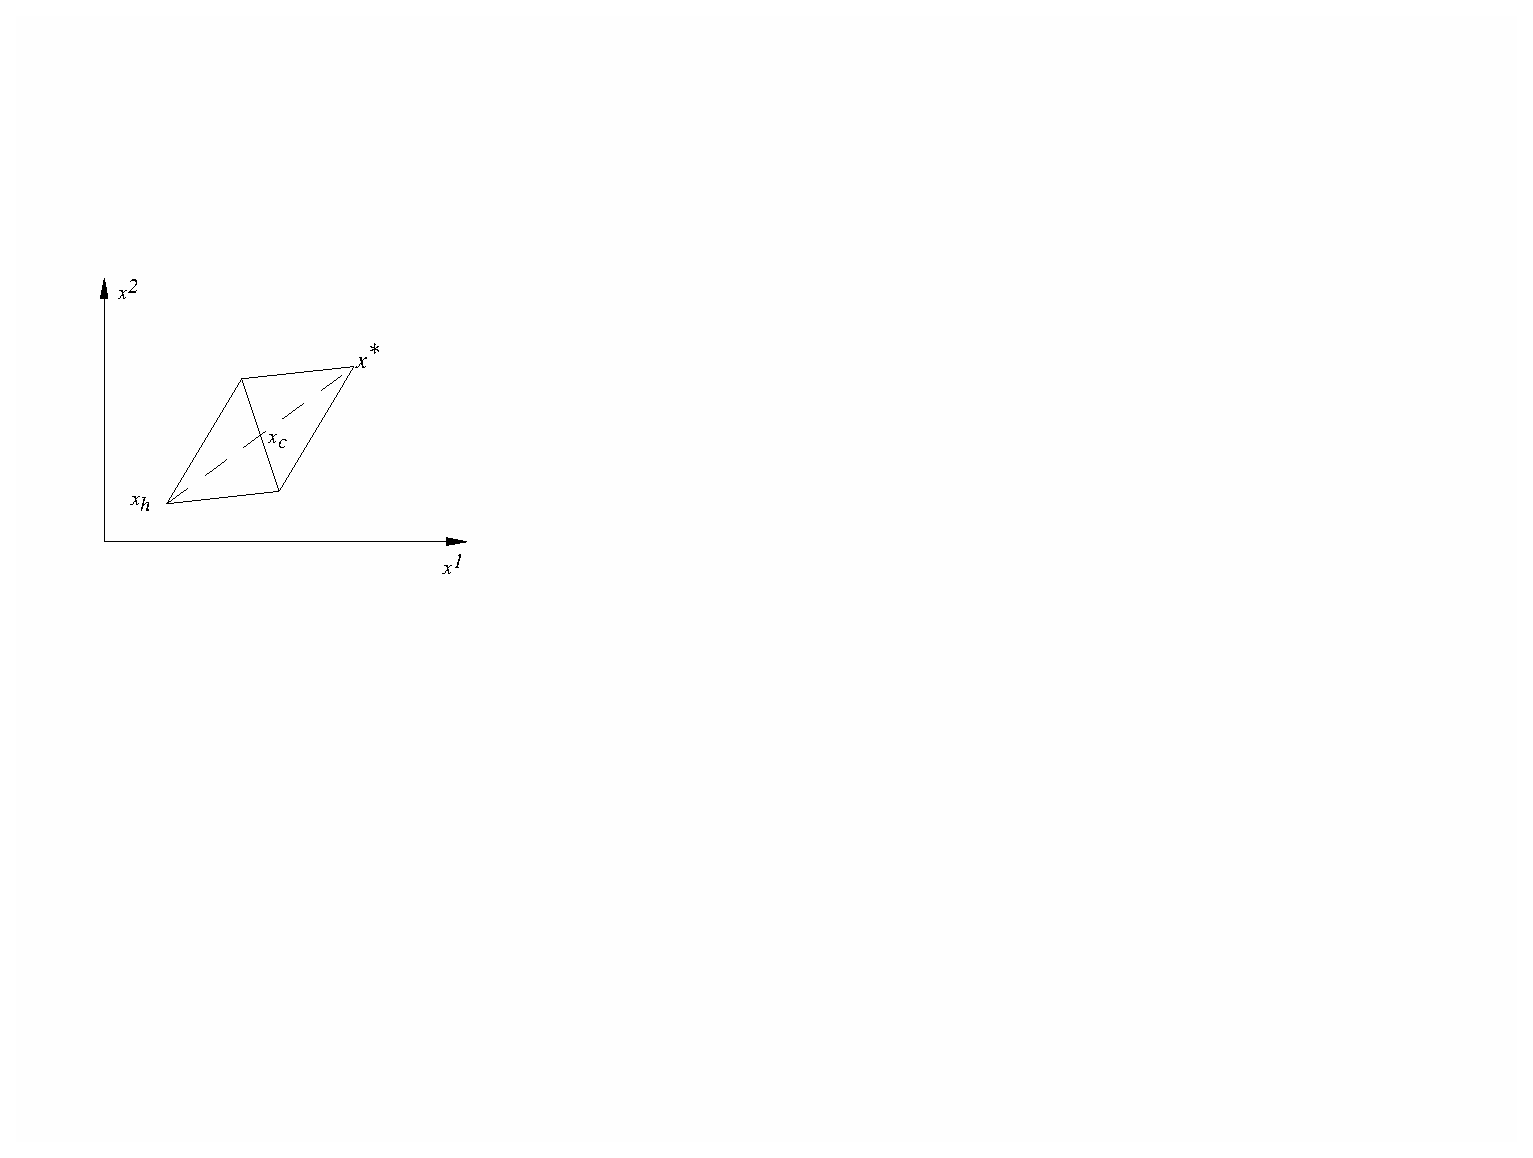
\epsfig
      {file=img/nel_mea_ref.eps, bb=35 265 225 420, scale=0.9, clip=}}
    \subfigure[Expansion.]{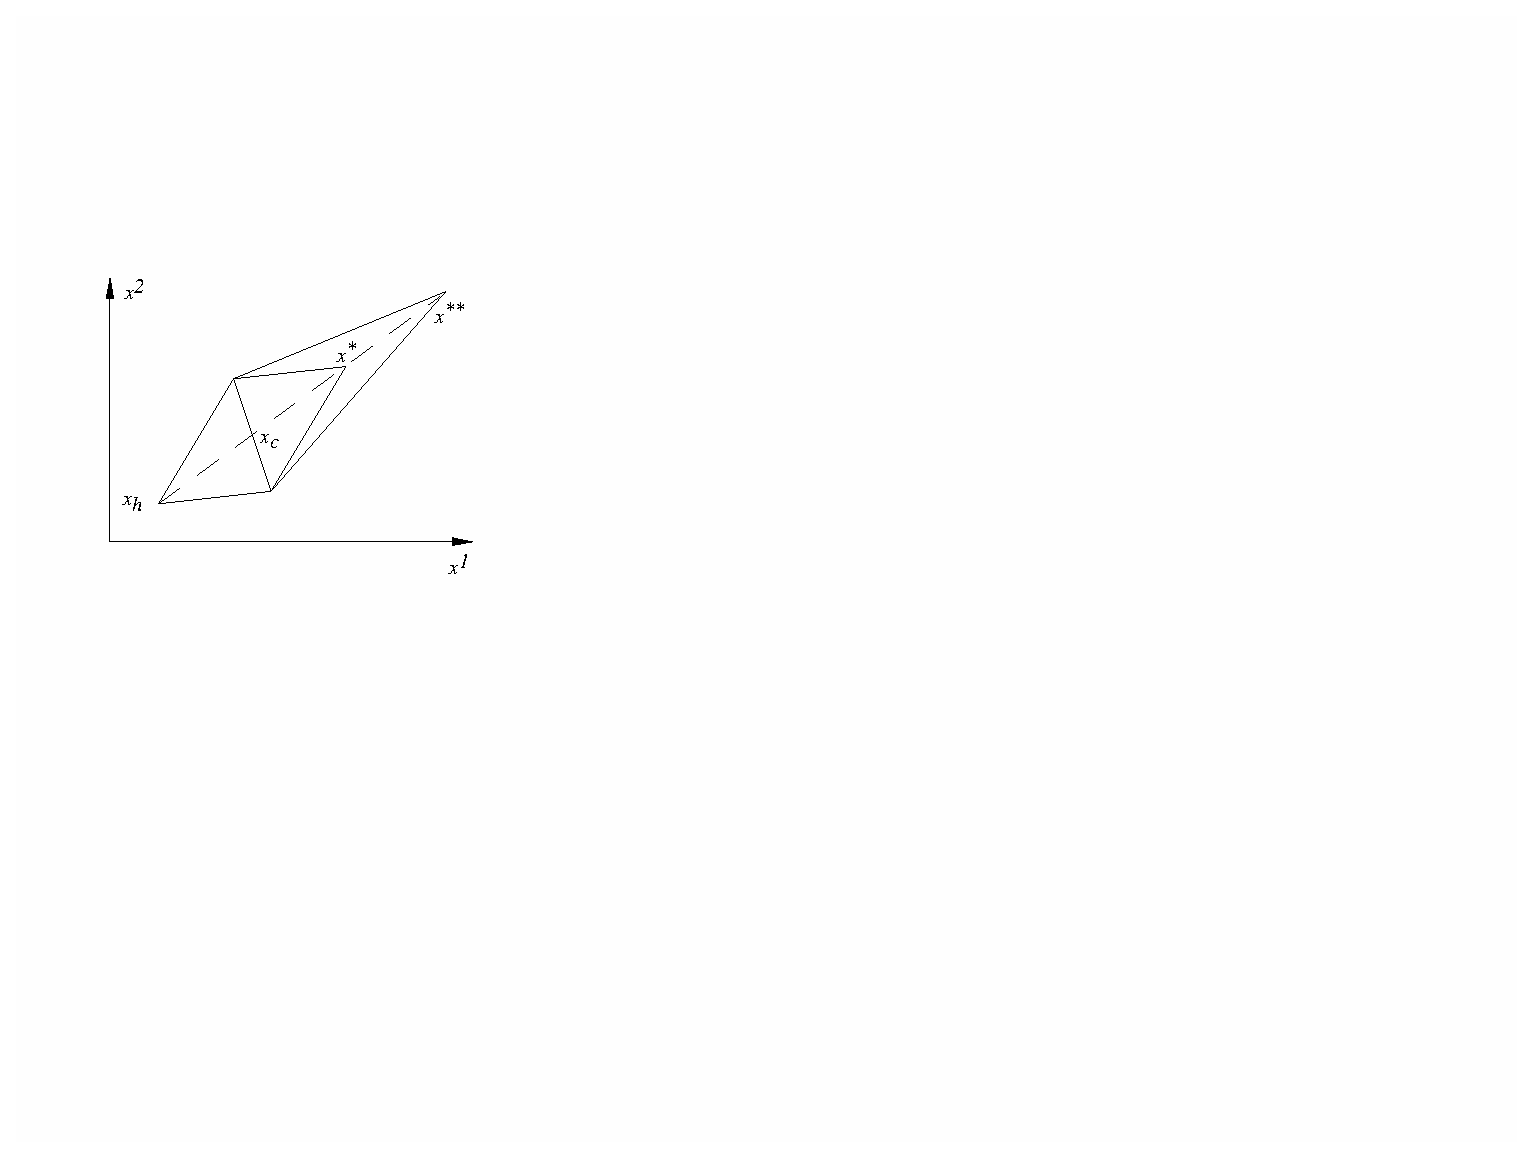
\epsfig
      {file=img/nel_mea_exp.eps, bb=35 265 225 420, scale=0.9, clip=}} }
  \mbox{ 
    \subfigure[Partial inside contraction.]{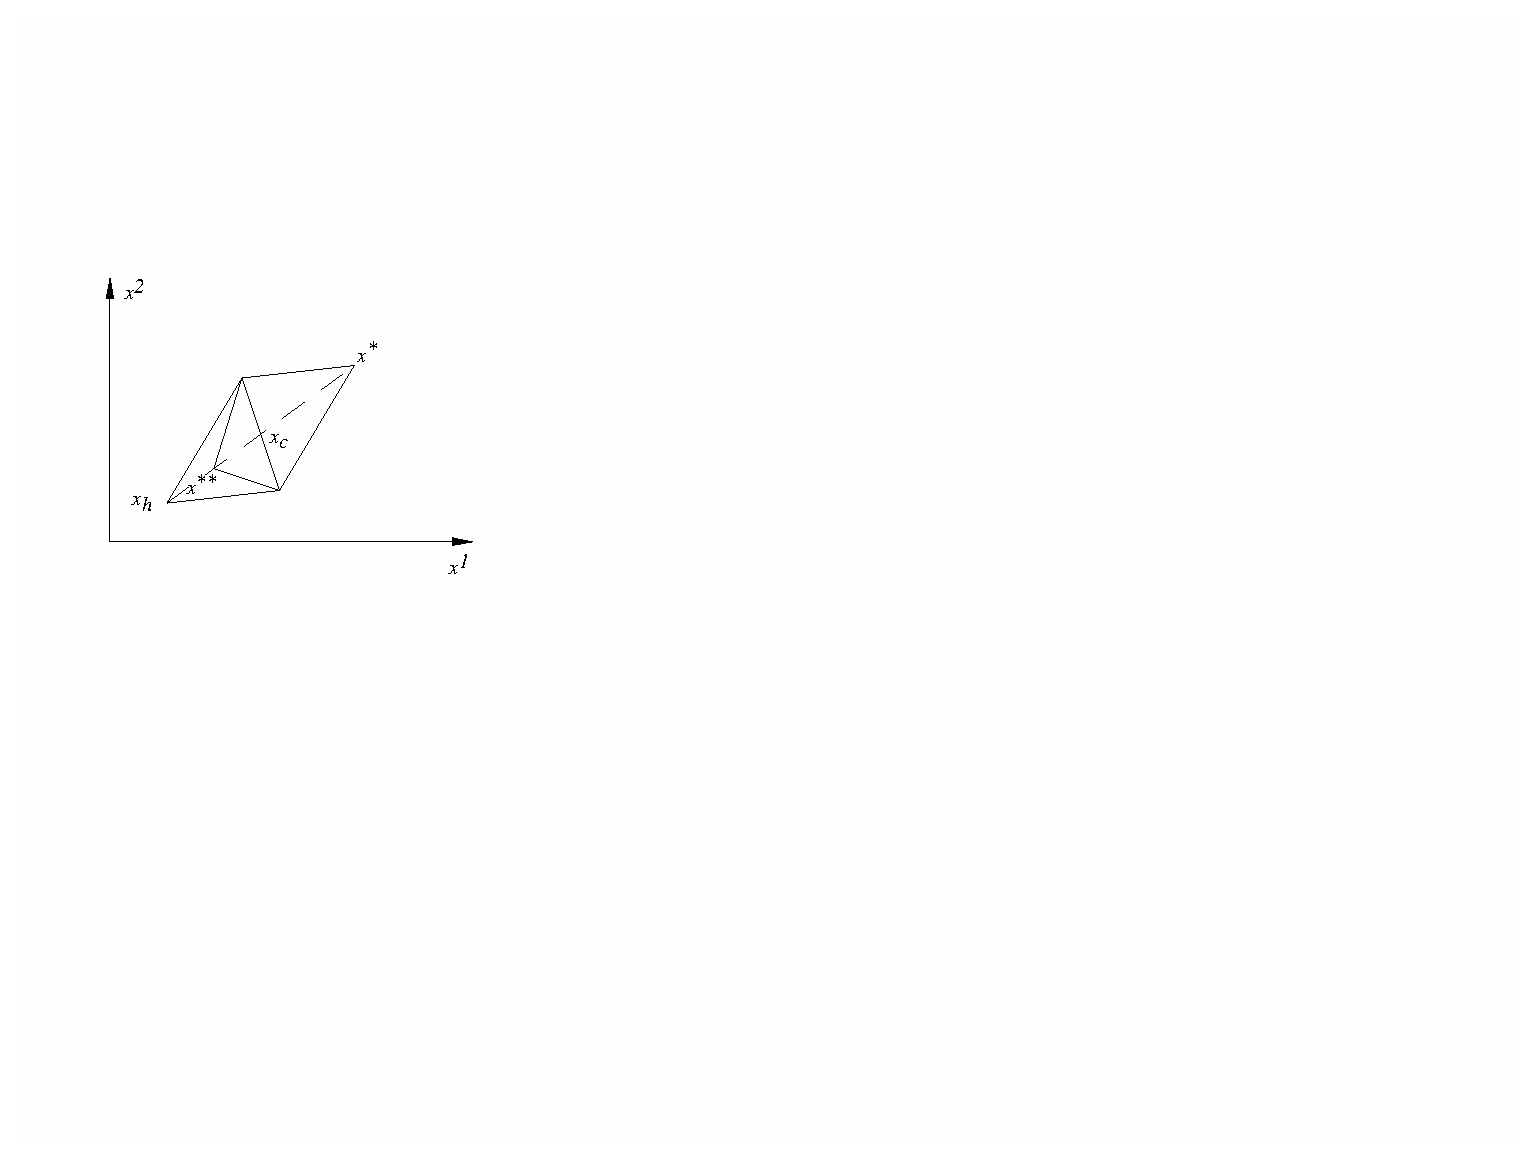
\epsfig
      {file=img/nel_mea_par_ins.eps, bb=35 265 225 420, scale=0.9, clip=}}
    \subfigure[Partial outside contraction.]{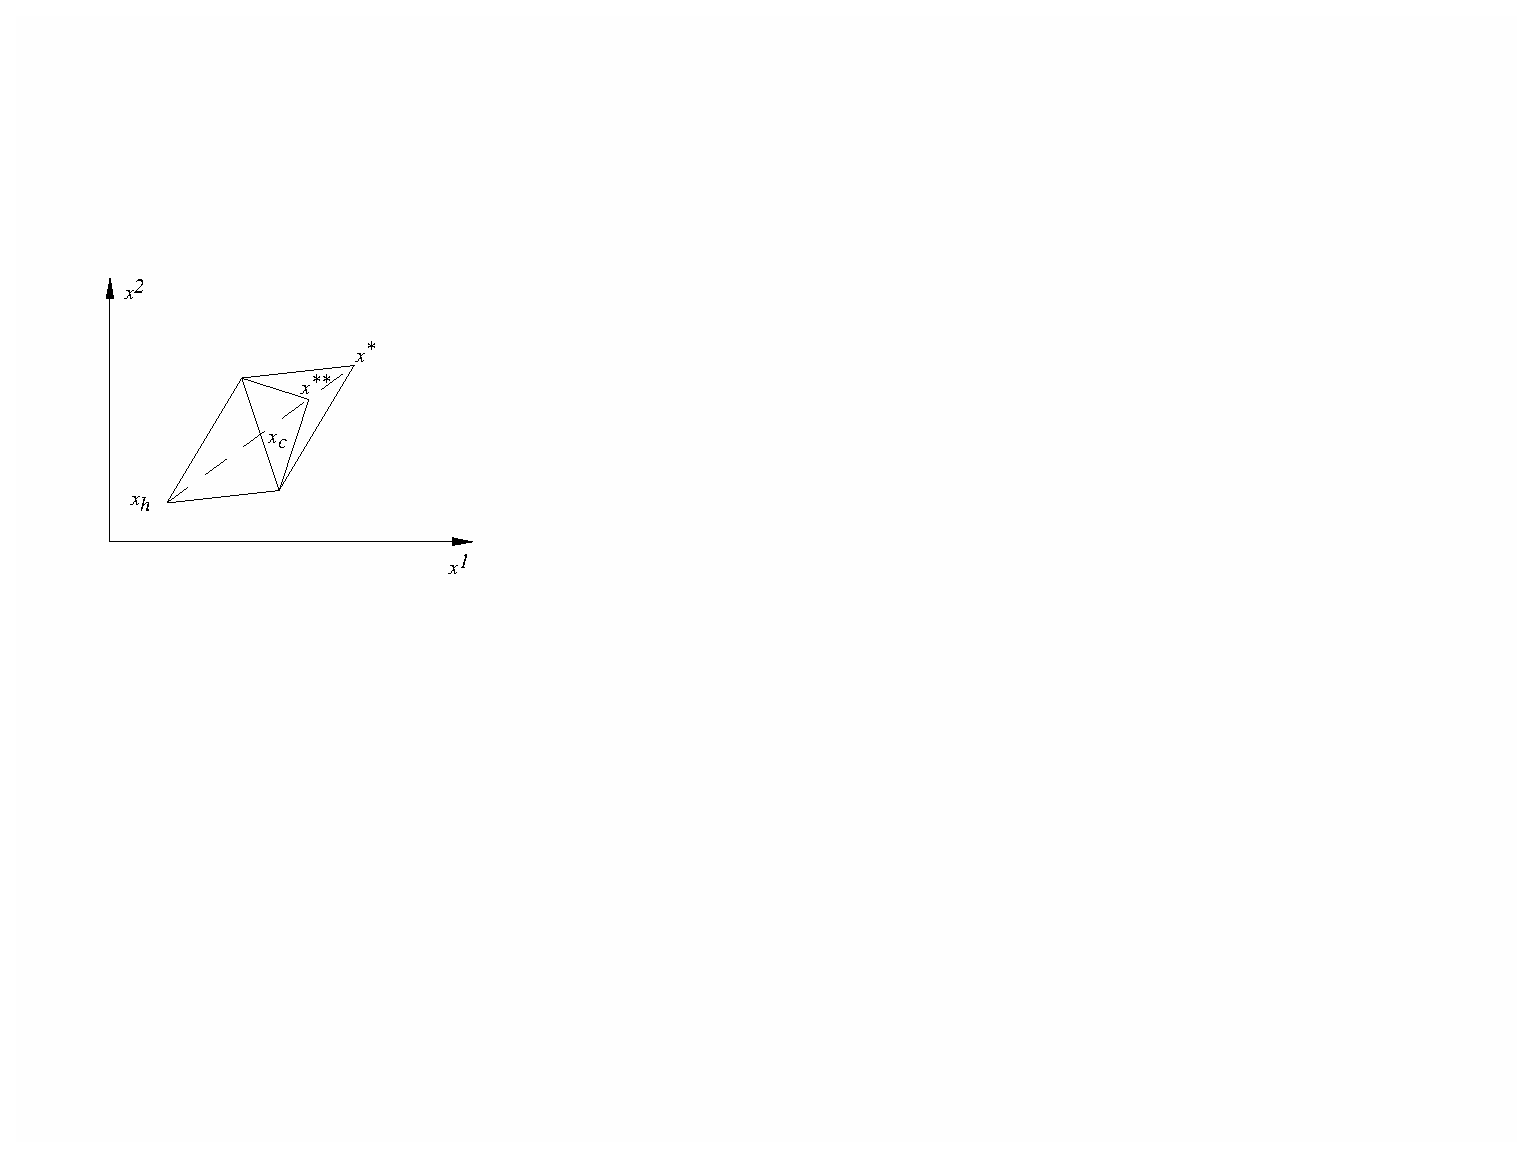
\epsfig
      {file=img/nel_mea_par_out.eps, bb=35 265 225 420, scale=0.9, clip=}} }
  \mbox{
    \subfigure[Total contraction.]{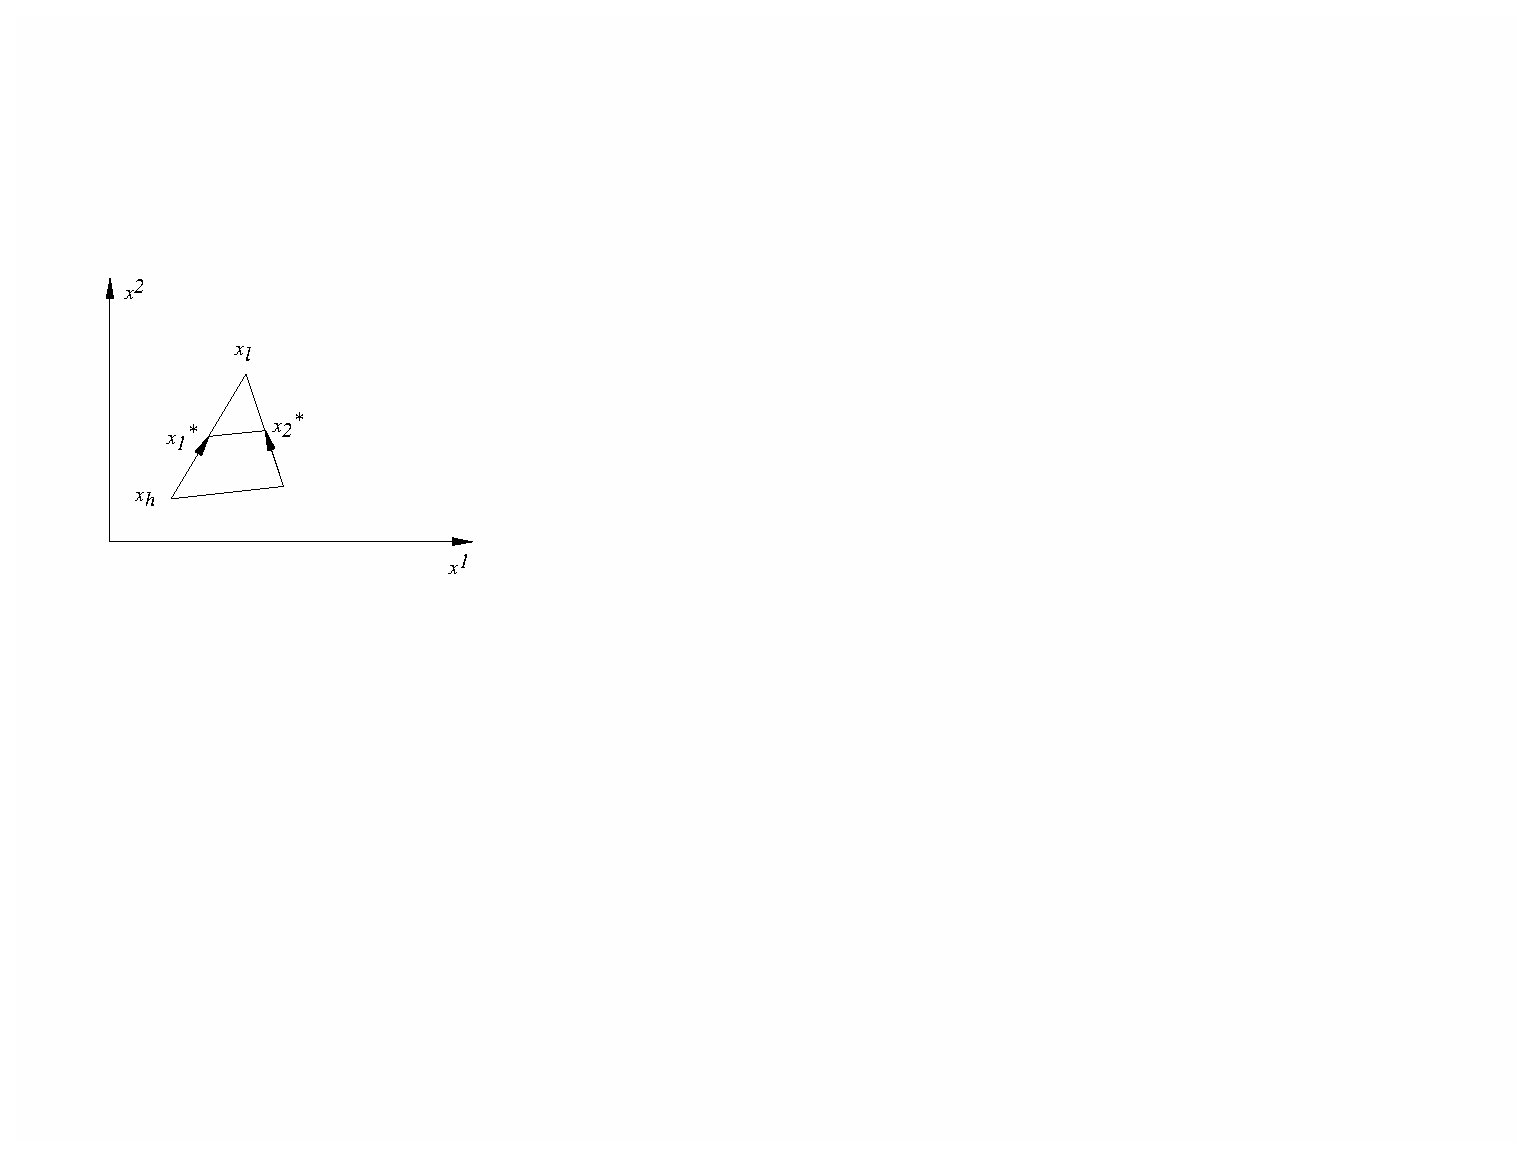
\epsfig
      {file=img/nel_mea_tot.eps, bb=35 265 225 420, scale=0.9, clip=}} }
  \caption{Simplex operations.}
  \label{fig:simOpeAll}
\end{figure}
The notation defined below is used in describing the main operations. The operations are illustrated in Fig.~\ref{fig:simOpeAll} where for simplicity 
a two-dimensional simplex is illustrated.\\

We now introduce some notation and definitions.
\begin{subequations}
\begin{enumerate}
\item We will denote by $\mathbf{I} \triangleq \{1, \, \ldots \, , \, n+1\}$
the set of all vertex indices.
\item
We will denote by $l \in \mathbf I$ the smallest index in $\mathbf I$
such that
\begin{equation}
l = \argmin_{i \in \mathbf{I} }  f(x_i).
\label{eq:simIndL}
\end{equation}
Hence, $f(x_l) \le f(x_i)$, for all $i \in \mathbf I$. 
\item
We will denote by $h \in \mathbf I$ the smallest index in $\mathbf I$
such that
\begin{equation}
h = \argmax_{i \in \mathbf{I} }  f(x_i).
\label{eq:simIndH}
\end{equation}
Hence, $f(x_h) \ge f(x_i)$, for all $i \in \mathbf I$. 
\item 
Let $x_i$, for $i \in \mathbf I$, denote the simplex vertices, and let $h$ be as in~\eqref{eq:simIndH}.
We will denote by $x_c \in \Re^n$ the {\em centroid} of the simplex, defined as
\begin{equation}
x_c \triangleq \frac{1}{n} \, 
\mathop{\sum_{i=1}}_{i \neq h}^{n+1} x_i
\label{eq:simCenDef}
\end{equation}
\end{enumerate}
\end{subequations}

Next, we introduce the three main operations.
\begin{subequations}
\begin{description}
\item[Reflection]
Let $h \in \mathbf I$ be as in~\eqref{eq:simIndH} and let
$x_c$ be as in~\eqref{eq:simCenDef}.
The reflection of $x_h \in \Re^n$ to a point denoted as 
$x^* \in \Re^n$ is defined as
\begin{equation}
   x^* \triangleq (1+\alpha) \, x_c - \alpha \, x_h,
\label{eq:simRefOpe}
\end{equation}
where $\alpha \in \Re$, with $\alpha > 0$, is
called the \emph{reflection coefficient}.

\item[Expansion of the simplex]
Let $x^* \in \Re^n$ be as in~\eqref{eq:simRefOpe} and
$x_c$ be as in~\eqref{eq:simCenDef}.
The expansion of $x^* \in \Re^n$ to a point denoted as 
$x^{**} \in \Re^n$ is defined as
\begin{equation}
   x^{**} \triangleq \gamma \, x^* + (1-\gamma) \, x_c,
\label{eq:simExp}
\end{equation}
where $\gamma \in \Re$, with $\gamma > 1$, is
called the \emph{expansion coefficient}.

\item[Contraction of the simplex]
Let $h \in \mathbf I$ be as in~\eqref{eq:simIndH} and
$x_c$ be as in~\eqref{eq:simCenDef}.
The contraction of $x_h \in \Re^n$ to a point denoted as 
$x^{**} \in \Re^n$ is defined as
\begin{equation}
   x^{**} \triangleq \beta \, x_h + (1 - \beta) \, x_c,
  \label{eq:simAlgCon}
\end{equation}
where $\beta \in \Re$, with $0 < \beta < 1$, is
called the \emph{contraction coefficient}.
\end{description}
\end{subequations}

% ---------------------------------
\subsection{Basic Algorithm}
In this section, we describe the basic Nelder and Mead algorithm~\cite{NelderMea1965}. 
The extension of O'Neill and the modified restart criterion are discussed later.
The algorithm is as follows:
\begin{enumerate}

\item Initialization: 
Given an initial iterate $x_1 \in \Re^n$,
a scalar $c$, with $c=1$ in the initialization,
a vector $s \in \Re^n$ with user-specified step sizes for each independent parameter,
and the set of unit coordinate vectors $\{ e_i \}_{i=1}^n$,
construct an initial simplex with vertices,
for $i \in \{1, \ldots , n \}$,
\begin{equation}
  x_{i+1} = x_1 + c \, s^i \, e_i.
\label{eq:simAlgIni}
\end{equation}
Compute $f(x_i)$, for $i \in \mathbf I$.
\item \label{des:simAlgRef} Reflection: 
Reflect the worst point, that is, compute $x^*$ as in~\eqref{eq:simRefOpe}.
\item \label{des:simAlgCheBes} Test whether we got the best point:
If $f(x^*) < f(x_l)$, expand the simplex using~\eqref{eq:simExp}
since further improvement in this direction is likely.
If $f(x^{**})< f(x_l)$, then 
$x_h$ is replaced by $x^{**}$,
otherwise $x_h$ is replaced by $x^*$, and 
the procedure is restarted from \ref{des:simAlgRef}.

\item 
If it turned out under \ref{des:simAlgCheBes} that $f(x^*) \ge f(x_l)$,
then we check if the new point $x^*$ is the worst of all points:
If $f(x^*) > f(x_i)$, for all $i \in \mathbf I$, with $i \ne h$, we contract 
the simplex (see \ref{des:simAlgCon}); 
otherwise we replace $x_h$ by $x^*$ and 
go to \ref{des:simAlgRef}.

\item \label{des:simAlgCon} 
For the contraction, we first check if we should try a partial outside 
contraction or a partial inside contraction: If $f(x^*) \ge f(x_h)$,
then we try a partial inside contraction.
To do so, we leave our indices as is and 
apply (\ref{eq:simAlgCon}). 
Otherwise, we try a partial outside contraction. 
This is done 
by replacing $x_h$ by $x^*$ and applying (\ref{eq:simAlgCon}). 
After the partial inside or the partial outside contraction,
we continue at \ref{des:simAlgCheWor}.

\item \label{des:simAlgCheWor}
If $f(x^{**}) \ge f(x_h)$\footnote{ Nelder and Mead~\cite{NelderMea1965} use the strict 
inequality $f(x^{**}) > f(x_h)$.
However, if the user writes the cost function value with only a few 
representative digits to a text file, 
then the function looks like a step function if slow convergence is 
achieved. In such cases, $f(x^{**})$ might sometimes be equal to $f(x_h)$.
Experimentally, it has been shown 
advantageous to perform a total contraction rather than continuing with a reflection. 
Therefore, the strict inequality has been changed to a weak inequality.},
we do a total contraction of the 
simplex by replacing $x_i \leftarrow (x_i + x_l)/2$, for all $i \in \mathbf I$.
Otherwise, we replace $x_h$ by $x^{**}$. 
In both cases, we continue from \ref{des:simAlgRef}.
\end{enumerate}

\begin{figure}
\centering
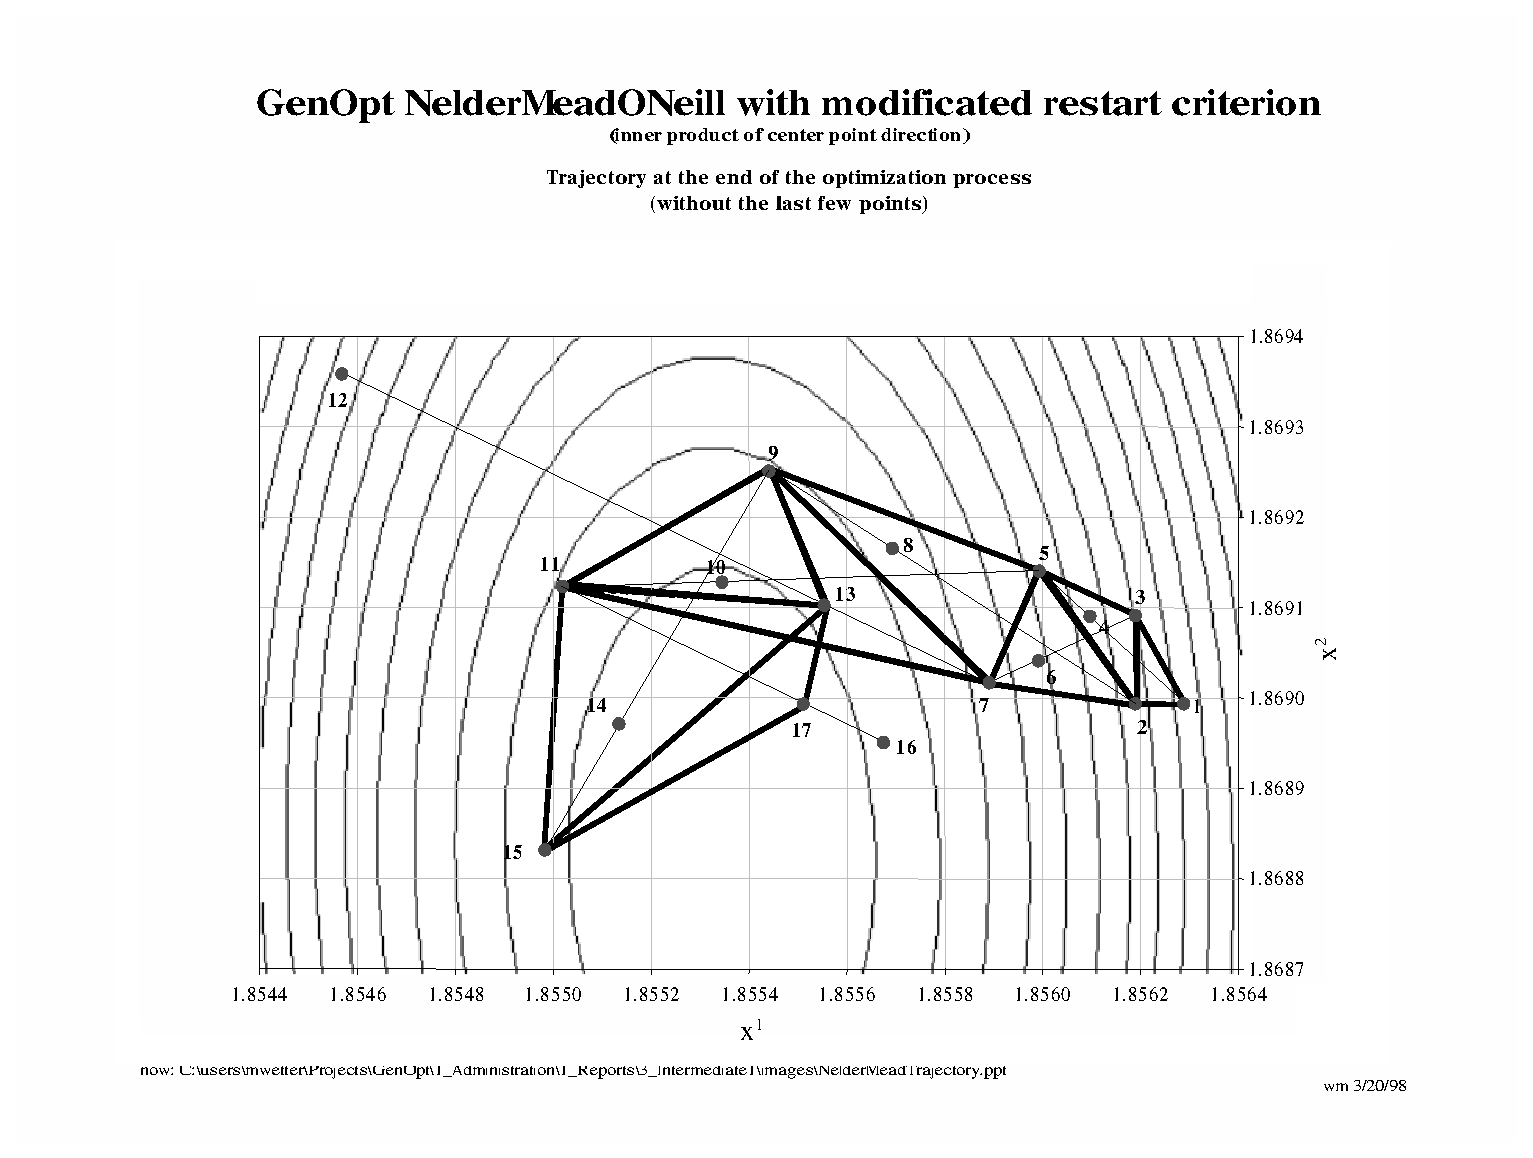
\epsfig{file=img/nel_mea_mov_tra.eps, bb=98 47 640 400, width=\headwidth, clip=}
\caption{Sequence of iterates generated by the Simplex algorithm.}
\label{fig:simSeqAlg}
\end{figure}



Fig. \ref{fig:simSeqAlg} shows a contour plot of a cost function $f \colon \Re^n \to \Re$ with a sequence of iterates
generated by the Simplex algorithm.
The sequence starts with 
constructing an initial simplex $x_1$, $x_2$, $x_3$. $x_1$ has the highest function value and is therefore 
reflected, which generates $x_4$. $x_4$ is the best point in the set $\{x_1, x_2, x_3, x_4\}$. Thus, it is further 
expanded, which generates $x_5$. $x_2$, $x_3$ and $x_5$ now span the new simplex. In this simplex, $x_3$ is the 
vertex with the highest function value and hence goes over to $x_6$ and further to $x_7$. The process of reflection 
and expansion is continued again two times, which leads to the simplex spanned by $x_7$, $x_9$ and 
$x_{11}$. $x_7$ goes over to $x_{12}$ which turns out to be the worst point. Hence, we do a partial inside 
contraction, which generates $x_{13}$. $x_{13}$ is better than $x_7$ so we use the simplex spanned by $x_9$, 
$x_{11}$ and $x_{13}$ for the next reflection. 
The last steps of the optimization are for clarity not shown.


% ---------------------------------

\subsection{Stopping Criteria}
The first criterion is a test of the variance of the function values at the vertices of the simplex
\begin{equation}
\frac{1}{n} \, \left(
\sum_{i=1}^{n+1} \bigl( f(x_i) \bigr)^2 -
   \frac{1}{n+1} \, \left(\sum_{i=1}^{n+1} f(x_i)    \right)^2 \, 
\right) < \epsilon^2,
 \label{eq:neaMeaVar}
\end{equation}
then the original implementation of the algorithm stops.
Nelder and Mead have chosen this stopping criterion based on the statistical problem
of finding the minimum of a sum of squares surface.
In this problem, the curvature near the minimum yields information about
the unknown parameters.
A slight curvature indicates a high sampling variance of the estimate.
Nelder and Mead argue that in such cases, there is no reason for finding 
the minimum point with high accuracy.
However, if the curvature is marked, 
then the sampling variance is low and a higher accuracy in determining the optimal parameter set is desirable.

Note that the stopping criterion~\eqref{eq:neaMeaVar} requires the variance
of the function values at the simplex vertices to be smaller 
than a prescribed limit.
However, if $f(\cdot)$ has large discontinuities, which has been observed
in building energy optimization problems~\cite{WetterWright2003:1},
then the test~\eqref{eq:neaMeaVar} may never be satisfied.
For this reason, among others, 
we do not recommend using this algorithm if the cost function
has large discontinuities.

\pagebreak[4]
% -------------------
\subsection{O'Neill's Modification}
O'Neill modified the termination criterion by adding a further condition~\cite{ONeill1971}. He checks 
whether any orthogonal step, each starting from the best vertex of the current simplex, leads to a further 
improvement of the cost function. 
He therefore sets $c = 0.001$ and tests if
\begin{subequations}
\label{eq:optCheNelMeaOri}
\begin{equation}
  f(x_l) < f(x)
\label{eq:optCheNelMeaOriCon}
\end{equation}
for all $x$ defined by
\begin{equation}
   x \triangleq x_l + c \, s^i \, e_i, \qquad i \in \{1, \ldots , n \},
  \label{eq:optCheNelMeaOriCoo}
\end{equation}
where $x_l$ denotes the best known point,
and $s^i$ and $e_i$ are as in \eqref{eq:simAlgIni}.\\

% ----------------------------
\subsection{Modification of Stopping Criteria}

In GenOpt, (\ref{eq:optCheNelMeaOri}) has been modified. It has been observed that users sometimes 
write the cost function value with only few representative digits to the output file. 
In such cases, 
(\ref{eq:optCheNelMeaOriCon}) is not satisfied if the write statement 
in the simulation program truncates 
digits so that the difference $f(x_l)-f(x)$, where $f\depd$ denotes the value that is
read from the simulation output file, is zero.
To overcome this numerical problem, 
(\ref{eq:optCheNelMeaOriCoo}) has been modified to
\begin{equation}
   x = x_l + \exp(j) \, c \, s^i \, e_i, \qquad i \in \{1, \ldots , n \}
\label{eq:optCheNelMeaOriMod}
\end{equation}
\end{subequations}
where for each direction $i \in \{1, \ldots , n \}$, 
the counter $j \in \Na$ is set to zero for the first trial and increased by one as long as 
$f(x_l) = f(x)$.

If (\ref{eq:optCheNelMeaOriCon}) fails for any direction, then $x$ computed by 
(\ref{eq:optCheNelMeaOriMod}) is the new starting point and a new simplex with side lengths $(c\, s^i)$, $i \in \{1, \ldots, n\}$, is constructed.
The point $x$ that failed (\ref{eq:optCheNelMeaOriCon}) is then used as the initial point $x_l$ in (\ref{eq:simAlgIni}).\\


\begin{figure}
  \mbox{ \subfigure[Sequence of iterates in the neighborhood of the minimum.]{
  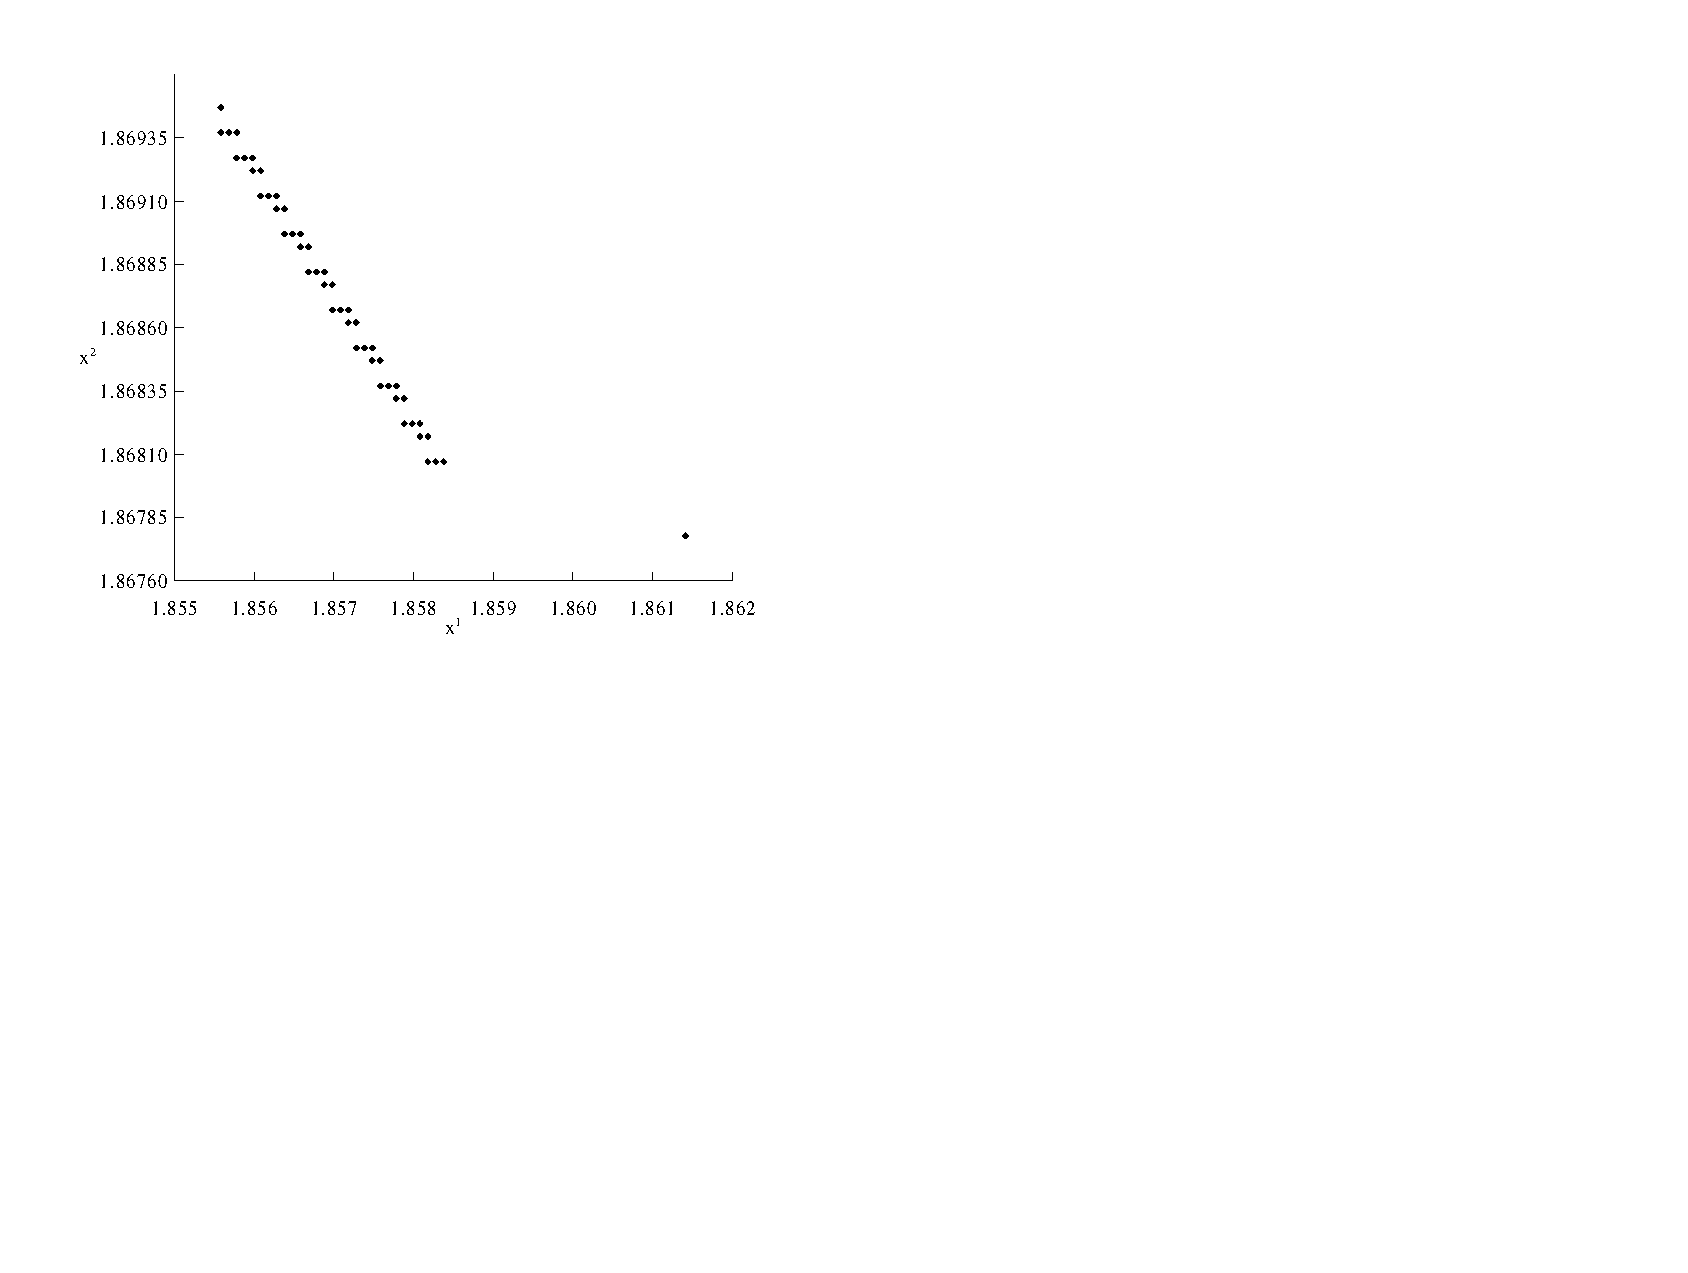
\epsfig{file=img/nel_mea_res_tra.eps, bb=25 290 360 575, clip=, width=0.5\headwidth} \label{fig:neaMeaResTra} } \quad
\subfigure[2-dimensional test function ``2D1''.]{
  \epsfig{file=img/fun_f2d1.eps, bb=120 95 740 500, width=0.5\headwidth} 
\label{fig:neaMeaTesFun} } }
\caption{Nelder Mead trajectory.}
\end{figure}
Numerical experiments showed that during slow convergence the algorithm was restarted too frequently.

Fig.~\ref{fig:neaMeaResTra} shows a sequence of iterates where the algorithm was restarted too frequently.
The iterates in the figure are part of the iteration sequence near the
minimum of the test function shown in Fig.~\ref{fig:neaMeaTesFun}. 
The algorithm gets close to the minimum with appropriately large steps.
The last of these steps can be seen at the right of the figure.
After this step, the stopping criterion (\ref{eq:neaMeaVar}) was satisfied 
which led to a restart check, followed by a new construction of the simplex. From there on, the 
convergence was very slow due to the small step size. After each step, the stopping criterion was satisfied 
again which led to a new test of the optimality condition (\ref{eq:optCheNelMeaOriCon}), followed by a 
reconstruction of the simplex. This check is very costly in terms of function evaluations and, furthermore, 
the restart with a new simplex does not allow increasing the step size, though we are heading locally in 
the right direction.\\

O'Neill's modification prevents both excessive checking of the optimality condition as well as excessive 
reconstruction of the initial simplex. This is done by checking for convergence only after a predetermined 
number of steps (e.g., after five iterations). 
However, the performance of the algorithm depends 
strongly on this number. As an extreme case, a few test runs were done where convergence was checked 
after each step as in Fig. \ref{fig:neaMeaResTra}. It turned out that in some cases no convergence was 
reached within a moderate number of function evaluations if $\epsilon$ in (\ref{eq:neaMeaVar}) is chosen 
too large, e.g., $\epsilon = 10^{-3}$ (see Tab. \ref{tab:nelMeaBenMarRes}).\\

\pagebreak[2]
To make the algorithm more robust, it is modified based on the following arguments:
\begin{enumerate}
\item
If the simplex is moving in the same direction in the last two steps, then the search is not 
interrupted by checking for optimality since we are making steady progress in the moving direction.
\item
If we do \emph{not} have a partial inside or total contraction immediately beyond us, then it is likely 
that the minimum lies in the direction currently being explored. 
Hence, we do not interrupt the search with a restart.
\end{enumerate}

These considerations have led to two criteria that both have to be satisfied to permit the convergence check according to (\ref{eq:neaMeaVar}), which might be followed by a check for optimality.\\

First, it is checked if we have done a partial inside contraction or a total contraction. If so, we 
check if the direction of the latest two steps in which the simplex is moving has changed by an angle of at 
least $(\pi / 2)$. 
To do so, we introduce the center of the simplex, defined by
\begin{equation}
  x_m \triangleq \frac{1}{n+1} \, \sum_{i=1}^{n+1} x_i,
\end{equation}
where $x_i$, $i \in \{ 1, \ldots, n\}$, are the simplex vertices.
We also introduce the normalized direction of the simplex between two steps,
\begin{equation}
  d_k \triangleq \frac{ x_{m, k} - x_{m, k-1} }
{ \| x_{m, k} - x_{m, k-1} \| },
\end{equation}
where $k \in \Na$ is the current iteration number.

We determine how much the simplex has changed its direction $d_k$ between two steps by 
computing the inner product $\langle d_{k-1}, d_k \rangle$. 
The inner product is equal to the cosine of the angle $d_{k-1}$ and $d_k$.
If
\begin{equation}
  \cos \phi_k = \langle d_{k-1}, \, d_k \rangle \le 0,
  \label{eq:nelMeaCosMov}
\end{equation}
then the moving direction of the simplex has changed by at least $\pi / 2$.
Hence, the simplex has changed the exploration direction.
Therefore, a minimum might be achieved and we need to test the variance of the 
vertices (\ref{eq:neaMeaVar}), possibly followed by a test of (\ref{eq:optCheNelMeaOriCon}).\\

%---
Besides the above modification, a further modification was tested: 
In some cases, a reconstruction of the simplex after a failed check (\ref{eq:optCheNelMeaOriCon})
yields to slow convergence.
Therefore, the algorithm was modified so that it continues at 
point \ref{des:simAlgRef} on page~\pageref{des:simAlgRef} without reconstructing the simplex after 
failing the test (\ref{eq:optCheNelMeaOriCon}).
However, reconstructing the simplex led in most of the benchmark tests to faster convergence. Therefore, 
this modification is no longer used in the algorithm.

\subsection{Benchmark Tests}
\label{sec:algSimBenTes}

\begin{table}
\newcolumntype{C}{>{\centering\arraybackslash}X}
\begin{tabularx}{\headwidth}{|p{2cm}|C|C|C|C|C|C|C|C|}
\hline
 & \multicolumn{8}{|c|}{Accuracy} \\ \cline{2-9}
& \multicolumn{4}{|c|}{$\epsilon = 10^{-3}$} & \multicolumn{4}{|c|}{$\epsilon = 10^{-5}$} \\ \hline
\raggedright Test function & Rosen-brock & 2D1 & Quad with I matrix & Quad with Q matrix & Rosen-brock & 2D1 & Quad with I matrix & Quad with Q matrix \\ \hline
\raggedright Original, with reconstruction &  137  &  120  &  3061  &  1075  &  139  &  109  &  1066  &  1165 \\ \hline
\raggedright Original, no reconstruction &  136  &  110  &  1436  &  1356  &  139  &  109  &  1433  &  1253 \\ \hline
\raggedright Modified, with reconstruction &  145  &  112  &  1296  &  1015  &  152  &  111  &  1060  &  1185 \\ \hline
\raggedright Modified, no reconstruction &  155  &  120  &  1371  &  1347  &  152  &  109  &  1359  &  1312 \\ \hline
\end{tabularx}
\caption{Comparison of the number of function evaluations for different implementations of the simplex algorithm. See Appendix for the definition of the function.}
\label{tab:nelMeaBenMarRes}
\end{table}

\begin{figure}
  \centering
  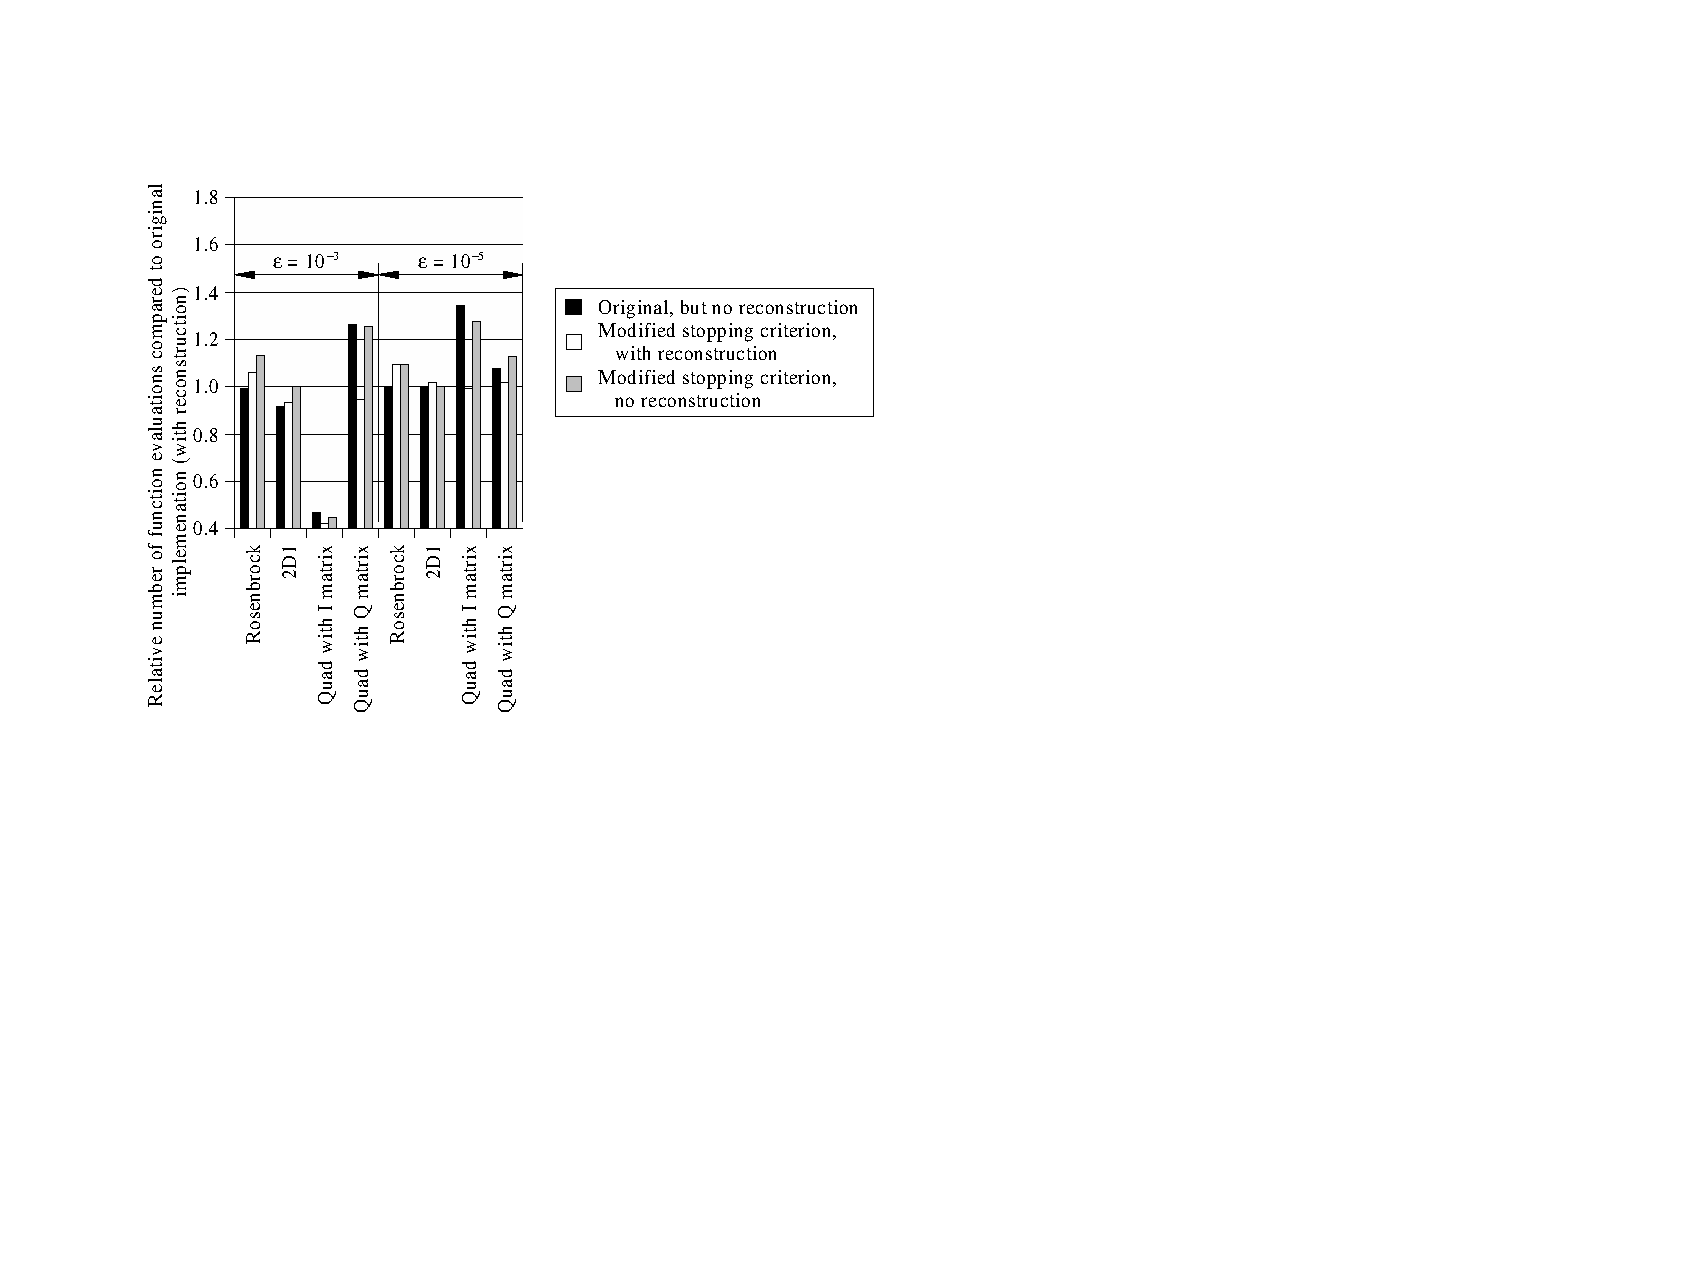
\epsfig{file=img/nel_mea_ben.eps, bb=60 255 420 520, clip=} 
  \caption{Comparison of the benchmark tests.}
  \label{fig:nelMeaBenMarRes}
\end{figure}

Tab.~\ref{tab:nelMeaBenMarRes} shows the number of function evaluations and 
Fig.~\ref{fig:nelMeaBenMarRes} shows the relative number of function evaluations compared to the original 
implementation for several test cases. The different functions and the parameter settings are given in the 
Appendix. 
The only numerical parameter that was changed for the different optimizations is the accuracy, $\epsilon$.\\

It turned out that modifying the stopping criterion is effective in most cases, 
particularly if a new simplex is constructed after the check~\eqref{eq:optCheNelMeaOriCon} failed.
Therefore, the following two versions of the simplex algorithm are implemented in GenOpt:
\begin{enumerate}
\item
The base algorithm of Nelder and Mead, including the extension of O'Neill.
After failing~\eqref{eq:optCheNelMeaOriCon},
the simplex is \emph{always} reconstructed with the new step size.
\item 
The base algorithm of Nelder and Mead, including the extension of O'Neill,
but with the modified stopping criterion as explained above.
That is, the simplex is only reconstructed if its moving direction changed, 
and if we have an inside or total construction beyond us.
\end{enumerate}

\subsection{Keywords}
For the Simplex algorithm, the command file (see page~\pageref{par:comFil}) must only contain continuous parameters.\\

To invoke the Simplex algorithm, the \texttt{Algorithm} section of the GenOpt command file must 
have following form:
\begin{lstlisting}
Algorithm{
   Main                    = NelderMeadONeill;
   Accuracy                = Double;   // 0 <  Accuracy
   StepSizeFactor          = Double;   // 0 <  StepSizeFactor
   BlockRestartCheck       = Integer;  // 0 <= BlockRestartCheck
   ModifyStoppingCriterion = Boolean;
}
\end{lstlisting}

\noindent The key words have following meaning:
\begin{codedescription}
\item[Main]
   The name of the main algorithm.
\item[Accuracy]
The accuracy that has to be reached before the optimality condition is checked. \texttt{Accuracy} is 
defined as equal to $\epsilon$ of (\ref{eq:neaMeaVar}), page~\pageref{eq:neaMeaVar}.

\item[StepSizeFactor]
A factor that multiplies the step size of each parameter for 
(a) testing the optimality condition and 
(b) reconstructing the simplex.
\texttt{StepSizeFactor} is equal to $c$ in 
(\ref{eq:simAlgIni}) and (\ref{eq:optCheNelMeaOriMod}).

\item[BlockRestartCheck]
Number that indicates for how many main iterations the restart criterion is not checked. If zero, restart 
might be checked after each main iteration.

\item[ModifyStoppingCriterion]
Flag indicating whether the stopping criterion should be modified. 
If \texttt{true}, then the optimality check 
(\ref{eq:neaMeaVar}) is done only if both of the following conditions are satisfied: 
(a) in the last step, either a partial inside contraction or total contraction was done, and 
(b) the moving direction of the simplex has changed by an angle $\phi_k$ of at least $(\pi/2)$, 
where $\phi_k$ is computed using (\ref{eq:nelMeaCosMov}).
\end{codedescription}



\chapter{Algorithms for One-Dimensional Optimization}
\label{sec:algOneDimOpt}
\section{Interval Division Algorithms}
\lab{sec:IntDivAlg}
Interval division algorithm can be used to minimize a function $f \colon \Re \to \Re$,
(i.e., the function depends on one independent parameter only,)
over a user-specified interval.
The algorithms do not require derivatives and 
they require only one function evaluation per interval division, 
except for the initialization.

First, we explain a master algorithm for the interval division algorithms.
The master algorithm is used to implement two commonly used interval division algorithms: 
The Golden Section search and the Fibonacci Division. 

\begin{figure}
\centering
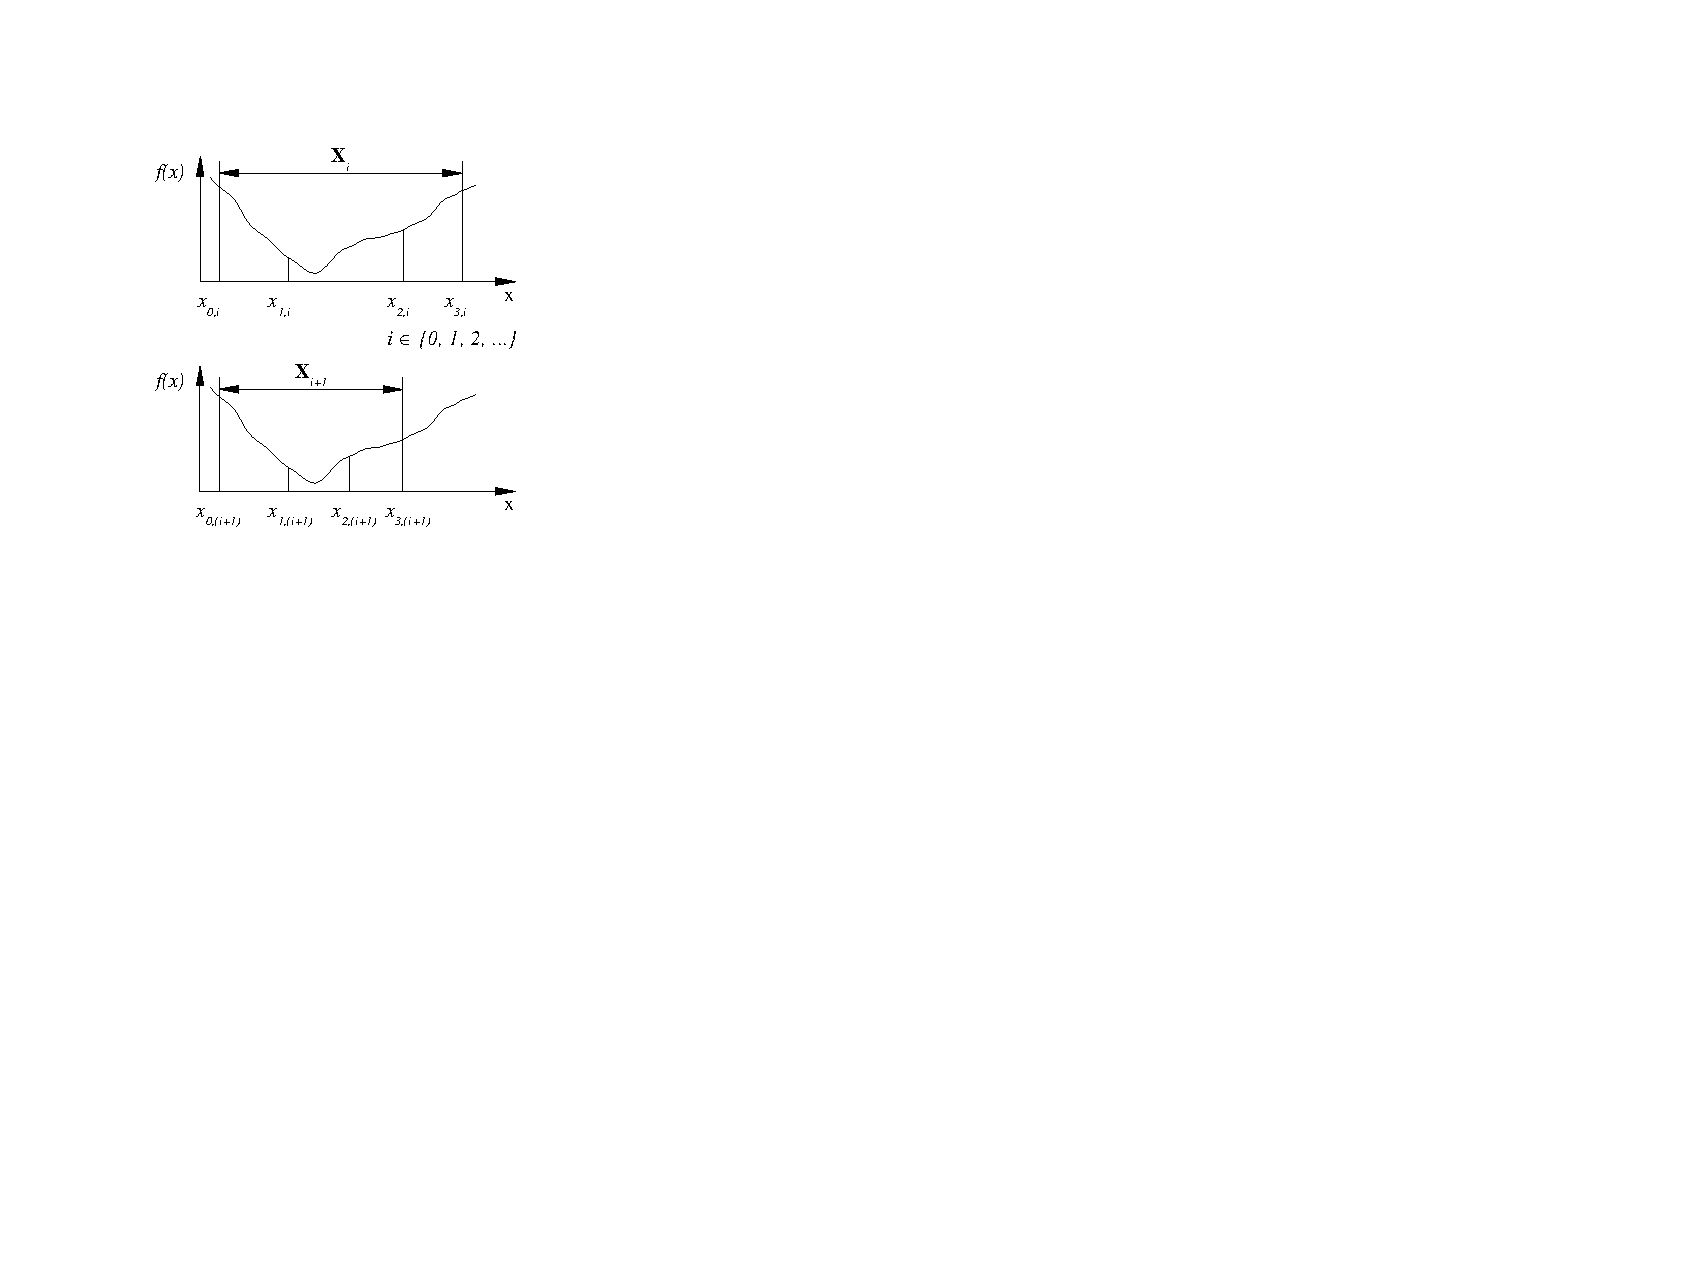
\epsfig{file=img/int_div.eps, bb=65 345 245 535}
\caption{Interval division.}
\label{fig:intDivGen}
\end{figure}

% --------
\subsection{General Interval Division}
We now describe the ideas behind the interval division methods.
For given $x_0, x_3 \in \Re$, with $x_0 < x_3$,
let $\mathbf X \triangleq [x_0, x_3]$.
Suppose we want to minimize $f(\cdot)$ on $\mathbf X$,
and suppose that $f \colon \Re \rightarrow \Re$ has a unique minimizer 
$x^* \in \mathbf X$.
For some $s \in (0, 1)$, let
\begin{eqnarray}
   x_1 & \triangleq & x_0 + s \, (x_3 - x_0), \\
   x_2 & \triangleq & x_1 + s \, (x_3 - x_1).
\end{eqnarray}
If $f(x_1) \le f(x_2)$, then $x^* \in  [x_0, \, x_2]$.
Hence, we can eliminate the interval $(x_2, \, x_3]$ 
and restrict our search to $[x_0, \, x_2]$.
Similarly, if $f(x_1) > f(x_2)$, then $x^* \in [x_1, \, x_3]$ 
and we can eliminate $[x_0, \, x_1)$.
Thus, we reduced the initial interval to a new interval that contains the minimizer $x^*$.\\

Let $i \in \Na$ be the iteration number.
We want to nest the sequence of intervals
\begin{equation}
[x_{0,(i+1)}, \, x_{3,(i+1)}] \subset [x_{0,i}, \, x_{3,i}], \qquad i \in \{0, \, 1, \, 2, \, \ldots \},
\end{equation}
such that we have to evaluate $f\depd$ in each step at one new point only.
To do so, we assign the new bounds of the interval such that either 
$[x_{0,(i+1)}, \, x_{3,(i+1)}] = [x_{0,i}, \, x_{2,i}]$, or $[x_{0, (i+1)}, \, x_{3, (i+1)}] = [x_{1,i}, \, x_{3,i}]$, 
depending on which interval has to be eliminated. 
By doing so, we have to evaluate only one new point in the interval. 
It remains to decide where to locate the new point.
The Golden Section and Fibonacci Division differ in this decision.

% --------
\subsection{Golden Section Interval Division}
Suppose we have three points $x_0 < x_1 < x_3$ in $\mathbf X \subset \Re$
such that for some $q \in (0, 1)$, to be determined later,
\begin{subequations}
\begin{equation}
   \frac{ | x_0 - x_1 | }{ | x_0 - x_3 |  } = q.
   \label{eq:golSecQDef}
\end{equation}
Hence,
\begin{equation}
   \frac{ | x_1 - x_3 | }{ | x_0 - x_3 |  } = 1-q.
\end{equation}
\end{subequations}

Suppose that $x_2$ is located somewhere between $x_1$ and $x_3$ and define
the ratio
\begin{equation}
  w \triangleq \frac{ | x_1 - x_2 | }{ | x_0 - x_3 |  }.
\end{equation}
Depending on which interval is eliminated, the interval in the next iteration step will
either be of length 
$(q+w) \, | x_0 - x_3|$, 
or $(1-q)  \, | x_0 - x_3|$.
We select the location of $x_2$ such that the two intervals are of the same length. 
Hence,
\begin{subequations}
\begin{equation}
   q + w = 1 - q.
  \label{eq:golSecqw}
\end{equation}
Now, we determine the fraction $q$.
Since we apply the process of interval division recursively, we know by scale similarity that
\begin{equation}
   \frac{ w }{ 1 - q } = q.
   \label{eq:golSecq}
\end{equation}
\end{subequations}
\begin{subequations}
Combining (\ref{eq:golSecqw}) and (\ref{eq:golSecq}) leads to
\begin{equation}
   q^2 - 3 q + 1 = 0,
\end{equation}
with solutions
\begin{equation}
   q_{1,2} = \frac{3 \pm \sqrt{5}}{2}.
\end{equation}
Since $q < 1$ by (\ref{eq:golSecQDef}), the solution of interest is
\begin{equation}
   q = \frac{3 - \sqrt{5}}{2} \approx 0.382.
\end{equation}
\end{subequations}

The fractional distances $q \approx 0.382$ and $1-q \approx 0.618$ correspond to the so-called \emph{Golden Section}, which gives this algorithm its name.\\

Note that the interval is reduced in each step by the fraction $1-q$, i.e., we have \emph{linear convergence}. In the $m$-th iteration, we have
\begin{eqnarray}
   | x_{ 0, \, m} - x_{ 2, \, m} | & = &
   | x_{ 1, \, m} - x_{ 3, \, m} | =
   | x_{ 0, \, (m+1)} - x_{ 3, \, (m+1)} | \nonumber \\
 & = &
   (1-q)^{m+1} \,    | x_{ 0, \, 0} - x_{ 3, \, 0} |.
\end{eqnarray}
Hence, the required number of iterations, $m$, to reduce the initial interval of uncertainty $|x_{0, \,0} - x_{3, \, 0} |$ to at least a fraction $r$, defined as
\begin{equation}
   r \triangleq \frac{ | x_{ 0, \, m} - x_{ 2, \, m} | }
                { | x_{ 0, \, 0} - x_{ 3, \, 0} | }
    = \frac{ | x_{ 1, \, m} - x_{ 3, \, m} | }
                { | x_{ 0, \, 0} - x_{ 3, \, 0} | },
  \label{eq:golSecDefR}
\end{equation}
is given by
\begin{equation}
  m = \frac{\ln r}{ \ln (1-q)} - 1.
\end{equation}


% =======================
\subsection{Fibonacci Division}
Another way to divide an interval such that we need one function evaluation per iteration can be constructed as follows: Given an initial interval $[x_{0, \, i}, x_{3, \, i}]$ , $i=0$, we divide it into three segments symmetrically around its midpoint. Let $d_{1,\, i} < d_{2,\, i} < d_{3,\, i}$ denote the distance of the segment endpoints, measured from $x_{0, \,i}$. Then we have by symmetry $d_{3,\, i}=d_{1,\, i} + d_{2,\, i}$. By the bracket elimination procedure explained above, we know that we are eliminating a segment of length $d_{1,\, i}$. Therefore, our new interval is of length $d_{3,\, (i+1)}= d_{2,\, i}$. By symmetry we also have $d_{3,\, (i+1)}= d_{1,\, (i+1)} + d_{2,\, (i+1)}$. Hence, if we construct our segment length such that $d_{3,\, (i+1)} = d_{1,\, (i+1)} + d_{2,\, (i+1)}= d_{2,\, i}$ we can reuse one known point. Such a construction can be done by using \emph{Fibonacci} numbers, which are defined recursively by
\begin{subequations}
\begin{eqnarray}
  F_0 & \triangleq & F_1 \triangleq 1, \\
  F_i & \triangleq & F_{i-1} + F_{i-2}, \qquad i \in \{2, \, 3, \, \ldots \}.
\end{eqnarray}
\end{subequations}
The first few numbers of the Fibonacci sequence are $\{1, \, 1, \,  2, \, 3, \, 5, \, 8, \, 13, \, 21, \, \ldots \}$. The length of the intervals $d_{1,\, i}$ and $d_{2, \, i}$, respectively, are then given by
\begin{equation}
   d_{1, \, i} = \frac{F_{m-i} }{ F_{m-i+2} }, \quad
  d_{2, \, i} = \frac{F_{m-i+1} }{ F_{m-i+2} }, \qquad
  i \in \{0, \, 1, \, \ldots \, , \, m \},
\end{equation}
where $m > 0 $ describes how many iterations will be done. Note that $m$ must be known prior to the first interval division. 
Hence, the algorithm must be stopped after $m$ iterations.\\

The reduction of the length of the uncertainty interval per iteration is given by
\begin{equation}
  \frac{ d_{3, \, (i+1)} }{  d_{3, \, i}  } =
  \frac{ d_{2, \, i} }{  d_{1, \, i} + d_{2, \, i}  } = 
   \frac{  \frac{ F_{m-i+1} }{F_{m-i+2}}  }
     {  \frac{F_{m-i}}{F_{m-i+2}} +  \frac{F_{m-i+1}}{F_{m-i+2}}   } = 
        \frac{ F_{m-i+1}   }{ F_{m-i+2}   }.
\end{equation}
After $m$ iterations, we have
\begin{eqnarray}
  \frac{d_{3, \, m}}{d_{3, \, 0}} & = & 
  \frac{ d_{ 3, \, m}  }{ d_{ 3, \, (m-1)}  } \, 
  \frac{ d_{ 3, \, (m-1)}  }{ d_{ 3, \, (m-2)}  } \,
   \ldots \,
   \frac{ d_{ 3, \, 2}  }{ d_{ 3, \, 1}  } \,
   \frac{ d_{ 3, \, 1}  }{ d_{ 3, \, 0}  } \nonumber \\
 & = &
  \frac{F_{2} }{ F_{3} } \, 
  \frac{F_{3} }{ F_{4} } \, \ldots \, 
  \frac{F_{m} }{ F_{m+1} } \, 
  \frac{F_{m+1} }{ F_{m+2} } 
=
  \frac{2}{F_{m+2}}.
\end{eqnarray}
The required number of iterations $m$ to reduce the initial interval $d_{3, \, 0}$ 
to at least a fraction $r$, defined by (\ref{eq:golSecDefR}), can again be obtained by expansion from
\begin{eqnarray}
  r & = & 
  \frac{d_{2, \, m}}{d_{3, \, 0}} = 
  \frac{ d_{ 3, \, (m+1)}  }{ d_{ 3, \, 0}  } = 
  \frac{ d_{ 3, \, (m+1)}  }{ d_{ 3, \, m}  } \,
  \frac{ d_{ 3, \, m}  }{ d_{ 3, \, (m-1)}  } \,
   \ldots \,
   \frac{ d_{ 3, \, 2}  }{ d_{ 3, \, 1}  } \,
   \frac{ d_{ 3, \, 1}  }{ d_{ 3, \, 0}  } \, \nonumber \\
 & = &
  \frac{F_{1} }{ F_{2} } \, 
  \frac{F_{2} }{ F_{3} } \, \ldots \, 
  \frac{F_{m} }{ F_{m+1} } \, 
  \frac{F_{m+1} }{ F_{m+2} } 
=
  \frac{1}{F_{m+2}}.
\end{eqnarray}
Hence, $m$ is given by
\begin{equation}
  m = \argmin_{m \in \Na} \left\{ m \ | \ r \ge \frac{1}{F_{m+2}} \right\}.
\end{equation}


% -----------------
\subsection{Comparison of Efficiency}
The Golden Section is more efficient than the Fibonacci Division. Comparing the reduction of the interval of uncertainty, $| x_{0, \, m} - x_{3, \, m}|$, in the limiting case for $m \rightarrow \infty$, we obtain
\begin{equation}
   \lim_{m \rightarrow \infty} \frac{ | x_{0, \, m} - x_{3, \, m}  |_{GS} }
  { | x_{0, \, m} - x_{3, \, m}  |_{F} }
= \lim_{m \rightarrow \infty} \frac{F_{m+2}}{2} \, (1-q)^m = 0.95.
\end{equation}

% --------------------

\subsection{Master Algorithm for Interval Division}
The following master algorithm explains the steps of 
the interval division algorithm.\\

\noindent
\begin{minipage}[b]{\textwidth}
\begin{algorithm}
[Model Interval Division Algorithm]
~\\
{\em
\begin{tabularx}{\headwidth}{m{2cm}l}
\multicolumn{2}{l}{\hspace{\textwidth}~} \\ \\[-8ex]\\
\hline \\[-2ex]
 \textbf{Data}: 
 & $x_0$, $x_3$. \\
 & Procedure that returns $r_i$, defined as\\
 & $r_i \triangleq |x_{0, \, i} - x_{2, \, i} | / |x_{0, \, 0} - x_{3, \, 0}|$. \\
\textbf{Step 0:} 
 & {\it Initialize }\\
  & $\Delta x = x_3 - x_0$,\\
  &$ x_2 = x_0 + r_1 \, \Delta x$,\\
  & $x_1 = x_0 + r_2 \, \Delta x$,\\
  & $f_1 = f(x_1)$, $ f_2 = f(x_2)$, and\\
  & $i = 2$.\\
\textbf{Step 1:} & {\it Iterate.}\\
  & Replace $i$ by $i + 1$.\\
  & If  $(f_2 < f_1)$\\
    &  \hspace{1cm}  Set  $x_0 = x_1$, $x_1 = x_2$,\\
    &   \hspace{1cm}   $f_1 = f_2$,\\
    &   \hspace{1cm}   $x_2 = x_3 - r_i \, \Delta x$, and\\
    &    \hspace{1cm}  $f_2 = f(x_2)$.\\
   & else\\
   &    \hspace{1cm} Set $x_3 = x_2$, $x_2 = x_1$,\\
   &    \hspace{1cm}  $f_2 = f_1$,\\
   &    \hspace{1cm}  $x_1 = x_0 + r_i \,  \Delta x$,\\
   &    \hspace{1cm}  $f_1 = f(x_1)$.\\
   \textbf{Step 2:} & Stop or go to Step 1.\\
   \hline \\
\end{tabularx}
}
\lab{al:ModOneDim}
\end{algorithm}
\end{minipage}
% ---------------------

\subsection{Keywords}
For the Golden Section and the Fibonacci Division algorithm, the command file (see page~\pageref{par:comFil}) must contain only one continuous parameter.\\

To invoke the Golden Section or the Fibonacci Division algorithm, the \texttt{Algorithm} Section of the GenOpt command file must have following form:
\begin{lstlisting}
Algorithm{
   Main              = GoldenSection | Fibonacci;
  [AbsDiffFunction   = Double;  |   // 0 < AbsDiffFunction
   IntervalReduction = Double;  ]   // 0 < IntervalReduction
}
\end{lstlisting}
\pagebreak[2]
\noindent The keywords have the following meaning
\begin{codedescription}
\item[Main]
The name of the main algorithm.
\end{codedescription}
The following two keywords are optional. If none of them is specified, then the algorithm stops after \texttt{MaxIte} function evaluations (i.e., after \texttt{MaxIte}$-2$ iterations), where \texttt{MaxIte} is specified in the section \texttt{OptimizationSettings}. If both of them are specified, an error occurs.
\begin{codedescription}
\item[AbsDiffFunction]
The absolute difference defined as
\begin{equation}
\Delta f \triangleq | \min \{ f(x_0),\, f(x_3) \} - \min \{ f(x_1), \, f(x_2) \}|.
\end{equation}
If $\Delta f$ is lower than \texttt{AbsDiffFunction}, the search stops successfully.\\
\underline{Note:} Since the maximum number of interval reductions must be known for the initialization of the Fibonacci algorithm, this keyword can be used only for the Golden Section algorithm. It must not be specified for the Fibonacci algorithm.
\item[IntervalReduction]
The required maximum fraction, $r$, of the end interval length relative to the initial interval length (see equation~\eqref{eq:golSecDefR}).
\end{codedescription}

\chapter{Algorithms for Parametric Runs}
\label{sec:algParRun}

The here described algorithms for 
parametric runs can be used to determine how sensitive a function is 
with respect to a change in the independent variables.
They can also be used to do a parametric
sweep of a function over a set of parameters.
The algorithm described in Section~\ref{sec:algParametric} varies one parameter at a time while holding all other parameters fixed at the value 
specified by the keyword \texttt{Ini}. The algorithm described in Section~\ref{sec:algParRunGen}, in contrast, constructs a mesh in the space of the independent parameters, and evaluates the objective function at each mesh point.

\section{Parametric Runs by Single Variation}
\lab{sec:algParametric}
\subsection{Algorithm Description}

The \texttt{Parametric} algorithm allows doing parametric runs where
one parameter at a time is varied and
all other parameters are fixed at their initial values
(specified by the keyword \texttt{Ini}).

Each parameter must have a lower and upper bound.
For the logarithmic scale, the lower and upper bounds must be bigger than zero.
To allow negative increments, the lower bound can be larger than the upper bound.
The absolute value of the keyword \texttt{Step} defines in how many intervals 
each coordinate axis will be divided.
If $\text{\texttt{Step}} < 0$, then the spacing is logarithmic; otherwise it is linear. Set $\text{\texttt{Step}} = 0$ to keep the parameter always fixed at the value
specified by \texttt{Ini}.

This algorithm can also be used with discrete parameters. This allows, for example, using a string to specify a window construction.
\\


The spacing is computed as follows:
For simplicity, the explanation is done for one parameter.
Let $l \triangleq \text{\texttt{Min}}$, $u \triangleq \text{\texttt{Max}}$ and $m \triangleq |\text{\texttt{Step}}|$,
where \texttt{Min}, \texttt{Max} and \texttt{Step} are specified in the command file.\\

\noindent
If $\text{\texttt{Step}} < 0$, we compute, for $i \in \{0, \ldots , m \}$,
\begin{subequations}
  \begin{eqnarray}
    p & = & \frac{1}{m} \, \log \frac{u}{l}, \\
    x_i & = & l \, 10^{p \, i}.
  \end{eqnarray}
If $\text{\texttt{Step}} > 0$, we compute, for $i \in \{0, \ldots , m \}$,
  \begin{equation}
    x_i = l + \frac{i}{m} \, (u-l).
  \label{eq:AlgParLinSpa}
  \end{equation}
  \label{subeq:AlgParSpa}
\end{subequations}

\begin{example}[Parametric run with logarithmic and linear spacing]
{\em
Suppose the parameter specification is of the form
\vspace{-0.5\baselineskip}
\begin{lstlisting}
Vary{
   Parameter{ Name = x1; Ini = 5; Step = -2; Min = 10; Max = 1000; }
   Parameter{ Name = x2; Ini = 3; Step = 1;  Min = 2;  Max = 20;   }
}
\end{lstlisting}
\vspace{-0.5\baselineskip}
and the cost function takes two arguments, $x_1, x_2 \in \Re$.
Then, the cost function will be evaluated at the points\\
\noindent $(x_1, x_2) \in \{ (10,3), \ (100,3), \ (1000,3), \ (5,2), \ (5,20) \}$.\rbox \\
}
\end{example}

\subsection{Keywords}
For this algorithm, the command file (see page~\pageref{par:comFil}) can contain continuous and discrete parameters.\\

The \texttt{Parametric} algorithm is invoked by the following specification in the command file:
\begin{lstlisting}
Algorithm{
   Main = Parametric;
   StopAtError = true | false;
}
\end{lstlisting}

\noindent The keywords have the following meaning:
\begin{codedescription}
\item[Main]
The name of the main algorithm.
\item[StopAtError]
If \texttt{true}, then the parametric run stops if a simulation error occurs. 
If \texttt{false}, then the parametric run does not stop if a simulation error occurs.
The failed function evaluation will be assigned the function value zero.
For information, an error message will be written to the user interface
and the optimization log file.
\end{codedescription}

% ===================================
\section{Parametric Runs on a Mesh}
\label{sec:algParRunGen}
\subsection{Algorithm Description}

In contrast to the algorithm \texttt{Parametric}, the algorithm \texttt{Mesh} spans a multi-dimensional grid in the space of the independent parameters, and it evaluates the objective function at each grid point.

Note that the number of function evaluations increases exponentially with the number 
of independent parameters.
For example, a $5$-dimensional grid with $2$ intervals in each dimension requires $3^5=243$ function evaluations, whereas a $10$-dimensional grid would require $3^{10}=59049$ function evaluations.\\

The values that each parameter can take on are computed in the same way
as for the algorithm \texttt{Parametric}. Therefore, the specification of a
\texttt{Parameter} underlies the same constraints as for the algorithm \texttt{Parametric}, which is described above.

\begin{example}[Parametric run on a mesh]~\\
{\em
Suppose the parameter specification is of the form
\vspace{-0.5\baselineskip}
\begin{lstlisting}
Vary{
  Parameter{ Name = x1; Min = -10; Ini = 99; Max = 10; Step = 1; } 
  Parameter{ Name = x2; Min = 1; Ini = 99; Max = 100; Step = -2; } 
}
\end{lstlisting}
\vspace{-0.5\baselineskip}
and the cost function takes two arguments, $x_1, x_2 \in \Re$.
Then, the cost function will be evaluated at the points\\
$(x_1, x_2) \in
\{(-10,\,  1)$,
$ ( 10, \, 1)$, 
$ (-10, \,  10)$, 
$ ( 10, \,  10)$, 
$ (-10, \, 100)$, 
$ ( 10, \, 100)\}$.

An alternative specification for $x_2$ that uses a discrete parameter and gives the same result is
\vspace{-0.5\baselineskip}
\begin{lstlisting}
Parameter{ 
  Name = x2; 
  Ini = "1"; 
  Values = "1, 10, 100";
} 
\end{lstlisting}
\vspace{-\baselineskip}
\rbox
}
\end{example}


\subsection{Keywords}

The \texttt{Mesh} algorithm is invoked by the following specification in the command file:
\begin{lstlisting}
Algorithm{
   Main        = Mesh;
   StopAtError = true | false;
}
\end{lstlisting}

\noindent The keywords have the following meaning:
\begin{codedescription}
\item[Main]
The name of the main algorithm.
\item[StopAtError]
If \texttt{true}, then the parametric run stops if a simulation error occurs. 
If \texttt{false}, then the parametric run does not stop if a simulation error occurs.
The failed function evaluation will be assigned the function value zero.
For information, an error message will be written to the user interface
and the optimization log file.
\end{codedescription}

\label{sec:algImpEnd}

\chapter{Constraints}
\label{cha:conGen}
For some optimization problems it is necessary to impose constraints 
on the independent variables and/or the dependent variables, as the following example shows.

\begin{example}{\em
Suppose we want to minimize the heating energy of a building, and suppose that
the normalized mass flow $\dot m$ of the heating system is an independent variable, with constraints
$0 \le \dot m \le 1$.
Without using constraints, the minimum energy consumption would be achieved 
for $\dot m = 0$, since then the heating system is switched off.
To solve this problem, we can impose a constraint on a dependent variable.
One possibility is to add a ``penalty'' term to the energy consumption. 
This could be such that every time a thermal comfort criterion 
(which is a dependent variable)
is violated, a large positive number is added to the energy consumption.
Thus, if $\mathrm{ppd}(x)$, with $\mathrm{ppd} \colon \Re^n \to \Re$, 
denotes the predicted percent of dissatisfied people (in percentage), and
if we require that $\mathrm{ppd}(x) \le 10 \%$, we could use the inequality constraint
$g(x) \triangleq \mathrm{ppd}(x) - 10 \le 0$.
}
\phantom{abc} \rbox
\end{example}

In Section~\ref{sec:boxConFre}, the method that is used in GenOpt to implement box constraints is 
described.
In Section~\ref{sec:conDepVarGen}, penalty and barrier methods that can be used to 
implement constraints on dependent variables are described.
They involve reformulating the cost function and, hence, are problem specific and 
have to be implemented by the user.

% ============================================
\section{Constraints on Independent Variables}
\label{sec:conFreParGen}
\subsection{Box Constraints}
\label{sec:boxConFre}

Box constraints are constant inequality constraints that define a feasible set as
\begin{equation}
\mathbf X \triangleq \bigl\{ x \in \Re^n \ | \ 
l^i \le x^i \le u^i, \ i \in \{1, \ldots, n \} \bigr\},
\end{equation}
where $-\infty \le l^i < u^i \le \infty$ for $i \in \{1, \ldots, n \}$.

In GenOpt, box constraints are either implemented directly 
in the optimization algorithm by setting $f(x) = \infty$ for unfeasible iterates,
or, for some algorithms, the independent variable $x \in \mathbf X$ is transformed 
to a new unconstrained variable which we will denote in this section by $t \in \Re^n$.

\begin{subequations}
Instead of optimizing the constrained variable $x \in \mathbf X$, 
we optimize with respect to the unconstrained variable $t \in \Re^n$.
The transformation ensures that all variables stay feasible during the iteration process.
In GenOpt, the following transformations are used:\\

\noindent
If $l^i \le x^i$, for some $i \in \{1, \ldots, n\}$,
\begin{eqnarray}
  t^i & = &\sqrt{x^i - l^i}, \\
  x^i & = &l^i + (t^i)^2.
\end{eqnarray}
If $l^i \le x^i \le u^i$, for some $i \in \{1, \ldots, n\}$, 
\begin{eqnarray}
  t^i & = & \arcsin\left( 
    \sqrt{\frac{x^i - l^i}{u^i-l^i}}
    \right), \\
 x^i & = &l^i + (u^i - l^i) \, \sin^2 t^i.
\end{eqnarray}
If $x^i \le u^i$, for some $i \in \{1, \ldots, n\}$,
\begin{eqnarray}
  t^i & = & \sqrt{u^i - x^i}, \\
   x^i & = & u^i - (t^i)^2.
\end{eqnarray}
\label{sub:traBoxCon}
\end{subequations}
% ----------------------------
\subsection{Coupled Linear Constraints}
In some cases the constraints have to be formulated in terms of a linear system of equations of the form
\begin{equation}
   A \, x = b,
\end{equation}
where $A \in \Re^m \times \Re^n$, $x \in \Re^n$, $b \in \Re^m$, and $\mathrm{rank}(A) = m$.\\

There are various algorithms that take this kind of restriction into account. However, such restrictions are rare in building simulation and thus not implemented in GenOpt. If there is a need to impose such restrictions, they can be included by adding an appropriate optimization algorithm and retrieving the coefficients by using the methods offered in GenOpt's class \texttt{Optimizer}.

% -----------------------------------------

\section{Constraints on Dependent Variables}
\label{sec:conDepVarGen}
We now discuss the situation where the constraints are non-linear and 
defined by
\begin{equation}
   g(x) \le 0,
\label{eq:conFunG}
\end{equation}
where $g \colon \Re^n \rightarrow \Re^m$ is once continuously differentiable.
\eqref{eq:conFunG} also allows formulating equality constraints of the form
\begin{equation}
  h(x) = 0,
\label{eq:equCon}
\end{equation}
for $h \colon \Re^n \to \Re^m$, which can be implemented by using penalty functions.
In example, one can define $g^i(x) \triangleq h^i(x)^2$ for $i \in \{ 1, \ldots, m \}$. Then, since $g^i(\cdot)$ is non-negative, the only feasible value is $g(\cdot) = 0$.
Thus, we will only discuss the case of inequality constraints of the form~\eqref{eq:conFunG}.\\

Such a constraint can be taken into account by adding \emph{penalty} or \emph{barrier} functions to the cost function, which are multiplied by a positive weighting factor $\mu$
that is monotonically increased (for penalty functions) or monotonically decreased to zero (for barrier functions).\\

We now discuss the implementation of barrier and penalty functions.
% ---------------------------
\subsection{Barrier Functions}
Barrier functions impose a punishment if the dependent variable gets close to the 
boundary of the feasible region.
The closer the variable is to the boundary, 
the higher the value of the barrier function becomes.

\noindent To implement a barrier function for $g(x) \le 0$,
where $g \colon \Re^n \to \Re^m$ is a continuously differentiable function whose
elements are strictly monotone increasing,
the cost function $f \colon \Re^n \to \Re$ can
be modified to
\begin{equation}
\widetilde f(x, \mu) \triangleq f(x) + \mu  \frac{1}{\sum_{i=1}^m g^i(x)}
\label{eq:barFun}
\end{equation}
where $\widetilde f \colon \Re^n \times \Re \to \Re$.
The optimization algorithm is then applied to the new function $\widetilde f(x,\mu)$.
Note that~\eqref{eq:barFun} requires that $x$ is in the interior of the feasible set\footnote{I.e., $x$ satisfies the strict inequality $g(x) > 0$.}.

\indent A drawback of barrier functions is that the boundary of the feasible set
can not be reached.
By selecting the weighting factors small, one can get close to the boundary. 
However, too small a weighting factor can cause the cost function to be ill-conditioned,
which can cause problems for the optimization algorithm.

Moreover, if the variation of the iterates between successive iterations is too big,
then the feasible boundary can be crossed. Such a behavior must be prevented
by the optimization algorithm, which can produce additional problems.\\


For barrier functions, one can start with a moderately large weighting factor $\mu$ 
and let $\mu$ tend to zero during the optimization process. 
That is, one constructs a sequence
\begin{equation}
  \mu_0 > \ldots > \mu_i > \mu_{i+1} > \ldots > 0.
  \label{eq:barFunWeiFac}
\end{equation}
Section~\ref{sec:ImpWeiFac} shows how $\mu_i$ can be computed in the coarse of the optimization.

Barrier functions do not allow formulating equality constraints of the form~\eqref{eq:equCon}.

% --------------------
\subsection{Penalty Functions}

In contrast to barrier functions, 
penalty functions allow crossing the boundary of the feasible set, and they allow
implementation of equality constraints of the form~\eqref{eq:equCon}. 
Penalty functions add a positive term to the cost function if a constraint is violated.

\noindent To implement a penalty function for $g(x) \le 0$, where
$g \colon \Re^n \to \Re^m$ is once continuously differentiable and each element is strictly
monotone decreasing,
the cost function $f \colon \Re^n \to \Re$ can
be modified to
\begin{equation}
\widetilde f(x, \mu) \triangleq f(x) + \mu  \sum_{i=1}^m \max(0,  g^i(x))^2,
\label{eq:penFun}
\end{equation}
where $\widetilde f \colon \Re^n \times \Re \to \Re$ is once continuously differentiable in $x$.
The optimization algorithm is then applied to the new function $\widetilde f(x,\mu)$.

As for the barrier method, selecting the weighting factor $\mu$ is not trivial.
Too small a value for $\mu$ produces too big a violation of the constraint.
Hence, the boundary of the feasible set can be exceeded by an unacceptable amount.
Too large a value of $\mu$ can lead to ill-conditioning of the cost function,
which can cause numerical problems.\\

The weighting factors have to satisfy
\begin{equation}
   0 < \mu_0 < \ldots < \mu_i < \mu_{i+1} < \ldots,
  \label{eq:penFunWeiFac}
\end{equation}
with $\mu_i \to \infty$, as $i \to \infty$.
See Section~\ref{sec:ImpWeiFac} for how to adjust $\mu_i$.
% ---------------------------------------

\subsection{Implementation of Barrier and Penalty Functions}
\label{sec:ImpWeiFac}

We now discuss how the weighting factors $\mu_i$ can be adjusted.
For $i \in \Na$, let $x^*(\mu_i)$ be defined as the solution
\begin{equation}
 x^*(\mu_i) \triangleq \arg \min_{x \in \mathbf X} \widetilde f(x, \mu_i),
\end{equation}
where $\widetilde f(x, \mu_i)$ is as in~\eqref{eq:barFun} or~\eqref{eq:penFun}, respectively.
Then, we initialize $i=0$, select an initial value $\mu_0 > 0$ and compute $x^*(\mu_0)$.
Next, we select a $\mu_{i+1}$ such that it satisfies~\eqref{eq:barFunWeiFac}
(for barrier functions) or~\eqref{eq:penFunWeiFac} (for penalty functions),
and compute $x^*(\mu_{i+1})$, using the initial iterate $x^*(\mu_i)$, and increase the counter 
$i$ to $i+1$.
This procedure is repeated until $\mu_i$ is sufficiently close to zero (for barrier functions)
or sufficiently large (for penalty functions).\\

To recompute the weighting factors $\mu_i$, 
users can request GenOpt to write a counter to the simulation input file, and then compute
$\mu_i$ as a function of this counter.
The value of this counter can be retrieved by 
setting the keyword \texttt{WriteStepNumber} in the optimization command file to \texttt{true},
and specifying the string \texttt{\%stepNumber\%} in the simulation input template file. 
GenOpt will replace the string \texttt{\%stepNumber\%} with the current counter value 
when it writes the simulation input file.
The counter starts with the value $1$ and its increment is $1$.\\

Users who implement their own optimization algorithm in GenOpt can call the method
\texttt{increaseStepNumber(...)} in the class \texttt{Optimizer} to increase the counter.
If the keyword \texttt{WriteStepNumber} in the optimization command file is set to \texttt{true}, the method calls the simulation to evaluate the cost function for the new value of this counter. If \texttt{WriteStepNumber} is \texttt{false}, no new function evaluation is performed by this method since the cost function does not depend on this counter.\\





\chapter{Program}
\label{sec:proIns}
GenOpt is divided into a kernel part and an optimization part.
The kernel reads the input files,
calls the simulation program,
stores the results,
writes output files, etc.
The optimization part contains the optimization algorithms.
It also contains classes of mathematical functions such as those used in linear algebra.\\

Since there is a variety of simulation programs and optimization algorithms, 
GenOpt has a simulation program interface and an optimization algorithm interface.
The simulation program interface allows using any simulation software to evaluate the cost function (see below for the requirements on the simulation program), and
allows implementing new optimization algorithms with little effort.

\section{Interface to the Simulation Program}
\begin{figure}
\centering
\scalebox{0.8}{ \input{prg_flow.pstex_t} }
\caption{Interface between GenOpt and the simulation program that evaluates the cost function.}
\end{figure}

Text files are used to exchange data with the simulation program and to specify how 
to start the simulation program.
This makes it possible to couple any simulation program to GenOpt without requiring code adaptation on either the GenOpt side or the simulation program side.
The simulation program must satisfy the following requirements:
\begin{enumerate}
\label{lis:simProIntReq}
\item 
The simulation program must read its input from one or more text files,
must write the value of the cost function to a text file, 
and must write error messages to a text file.
\item
It must be able to start the simulation program by a command and 
the simulation program must terminate automatically.
This means that the user does not have to open the input file manually 
and shut down the simulation program once the simulation is finished.
\end{enumerate}

The simulation program may be a commercially available program or one written by the user.
% -------------------------------------------------------------------------

% -------------------------------------------------------------------------
\section{Interface to the Optimization Algorithm}
\begin{figure}
\centering
\scalebox{0.8}{ \input{alg_inte.pstex_t} }
\caption{Implementation of optimization algorithms into GenOpt.}
\label{fig:algImp}
\end{figure}
The large variety of optimization algorithms led to the development of
an open interface that allows easy implementation of optimization algorithms.
Users can implement their own algorithms and add them to the library of available optimization algorithms without having to adapt and recompile GenOpt.
To implement a new optimization algorithm,
the optimization algorithm must be written according to the guidelines 
of Section~\ref{sec:impNewOptAlg}.
Thus, GenOpt can not only be used to do optimization with built-in algorithms, 
but it can also be used as a framework for developing, testing and comparing 
optimization algorithms.\\

Fig.~\ref{fig:algImp} shows GenOpt's program structure.
The class \texttt{Optimizer} is the superclass of each optimization algorithm. 
It offers all the functions required for retrieval of parameters that specify 
the optimization settings, performing the evaluation of the cost function and reporting results. 
For a listing of its methods, 
see \url{http://SimulationResearch.lbl.gov} or the Javadoc code documentation 
that comes with GenOpt's installation.

% ------------
\section{Package \texttt{genopt.algorithm}}
The Java package \texttt{genopt.algorithm} consists of all classes that contain
mathematical formulas that are used by the optimization algorithm.
The following packages belong to \texttt{genopt.algorithm}.
\begin{codedescription}
\item[genopt.algorithm]
This package contains all optimization algorithms. 
The abstract class \texttt{Optimizer}, which must be inherited 
by each optimization algorithm, is part of this package.

\item[genopt.algorithm.util.gps] contains 
a model Generalized Pattern Search optimization algorithm.

\item[genopt.algorithm.util.linesearch] contains 
classes for doing a line search along a given direction.

\item[genopt.algorithm.util.math] contains 
classes for mathematical operations.

\item[genopt.algorithm.util.optimality] contains 
classes that can be used to check 
whether a variable value is at a minimum point or not.

\item[genopt.algorithm.util.pso] contains 
a model Particle Swarm Optimization algorithm.

\end{codedescription}
These packages are documented in the Javadoc source code documentation
that comes with GenOpt's.

% -------------------------------------------------------------
\section{Implementing a New Optimization Algorithm}
\label{sec:impNewOptAlg}
To implement a new optimization algorithm,
you must write a Java class that has 
the syntax shown in Fig. \ref{fig:codAlgStrGen}.
The class must use the methods of the abstract class \texttt{Optimizer} 
to evaluate the cost function and to report the optimization steps.
The methods of the \texttt{Optimizer} class are documented
in the Javadoc source code documentation.\\

Follow these steps to implement and use your own optimization algorithm:
\begin{enumerate}
\item 
Put the byte-code (\texttt{{\it ClassName}.class}) in the directory \texttt{genopt/algorithm}.
\item 
Set the value of the keyword \texttt{Main} in the \texttt{Algorithm} section of the optimization command file to the name of the optimization class (without file extension).
\item 
Add any further keywords that the algorithm requires 
to the \texttt{Algorithm} section. 
The keywords must be located \emph{after} the entry \texttt{Main} of the optimization command file. The keywords must be in the same sequence as they are called in the optimization code.
\item 
Call the method \texttt{Optimizer.report(final Point, final boolean)} 
after evaluating the cost function. 
Otherwise, the result will not be reported.
\item 
Call either the method \texttt{Optimizer.increaseStepNumber()}
or the method
\texttt{Optimizer.increaseStepNumber(final Point)}
after the optimization algorithm converged to some point.
These methods increase a counter that can be used to add penalty or 
barrier functions to the cost function.
In particular, the methods \url{Optimizer.increaseStepNumber()}
and \url{Optimizer.increaseStepNumber(final Point)} increase the
variable \texttt{stepNumber} (see Section~\ref{cha:conGen}) by one.
\end{enumerate}


\begin{figure}[ht!]
\centering
\begin{alltt}
\codeem{package genopt.algorithm;

import genopt.GenOpt;
import genopt.lang.OptimizerException;
import genopt.io.InputFormatException;

public class ClassName extends Optimizer\{

   public ClassName (GenOpt genOptData)
      throws InputFormatException, OptimizerException, 
             IOException, Exception
   \{ }
      // set the mode to specify whether the
      // default transformations for the box
      // constraints should be used or not \codeem{
      int constraintMode = xxxx;
      super(genOptData, constraintMode);}

      // remaining code of the constructor
   \codeem{\}

   public int run() throws OptimizerException, IOException
   \{ }
      // the code of the optimization algorithm \codeem{
   \}}

   // add any further methods and data members
\codeem{\}}
\end{alltt}
   \caption{Code snippet that specifies how to implement an optimization algorithm.}
   \label{fig:codAlgStrGen}
\end{figure}




\chapter{Installing and Running GenOpt}
\label{sec:InsAndRunGen}
\section{System Requirements}
To run GenOpt and the GenOpt installation program, a Java \javaversion runtime environment is required.
GenOpt should run on any operating system that can run Java applications.

\section{Installing and uninstalling GenOpt}
To install GenOpt, download the installation program
{\tt genopt-install.jar} from
\url{http://SimulationResearch.lbl.gov/GO}.
Then, either double-click on the file {\tt genopt-install.jar}\footnote{Depending on your Java installation, the file extension {\tt jar} may not be associated with Java. In this situation, please consult the instructions of your operating system for how to associate file extensions with programs.}
or open a command shell, change to the directory that contains {\tt genopt-install.jar} and type
\begin{lstlisting}
  java -jar genopt-install.jar
\end{lstlisting}
No environment variables need to be set to run GenOpt. (This is new since GenOpt~2.1.0.)

Note that Windows~7, depending on the permission of the user account, may not allow the GenOpt installation program to install GenOpt in {\tt C:\textbackslash Program Files}. In this situation, GenOpt can be installed in another programs, and then moved to {\tt C:\textbackslash Program Files}.\\

To uninstall GenOpt, delete the directory in which GenOpt was installed.

% ----------------------------------------------------------
\section{Running GenOpt}
\subsection{Running GenOpt from the file explorer}
To run GenOpt from the file explorer,
double-click on the file {\tt genopt.jar}.$^1$
This will start the graphical user interface. 
From the graphical user interface, select {\tt File},
{\tt Start...} and select a GenOpt initialization file.

\subsection{Running GenOpt from the command line}
GenOpt can also be run as a console application, either with or without the graphical user interface. 
To run GenOpt as a console application with the graphical user interface, open a shell, change to the directory that contains
{\tt genopt.jar} and type
\begin{lstlisting}
  java -jar genopt.jar [initializationFile]
\end{lstlisting}
where {\tt [initializationFile]} is an optional argument that can be
replaced with the GenOpt initialization file (see example below).
To start GenOpt without the graphical user interface, type
\begin{lstlisting}
  java -classpath genopt.jar genopt.GenOpt [initializationFile]
\end{lstlisting}
\newpage
For instance, to run the example file provided with GenOpt that minimizes a quadratic function using the Hooke-Jeeves algorithm, 
type on Mac OS~X
\begin{lstlisting}
  java -jar genopt.jar example/quad/GPSHookeJeeves/optMacOSX.ini
\end{lstlisting}
on Linux
\begin{lstlisting}
  java -jar genopt.jar example/quad/GPSHookeJeeves/optLinux.ini
\end{lstlisting}
and on Windows 
\begin{lstlisting}
  java -jar genopt.jar example\quad\GPSHookeJeeves\optWinXP.ini
\end{lstlisting}
This should produce the window shown in Fig.~\ref{fig:wingenoptGPSHJ}.

\begin{figure}
\centering
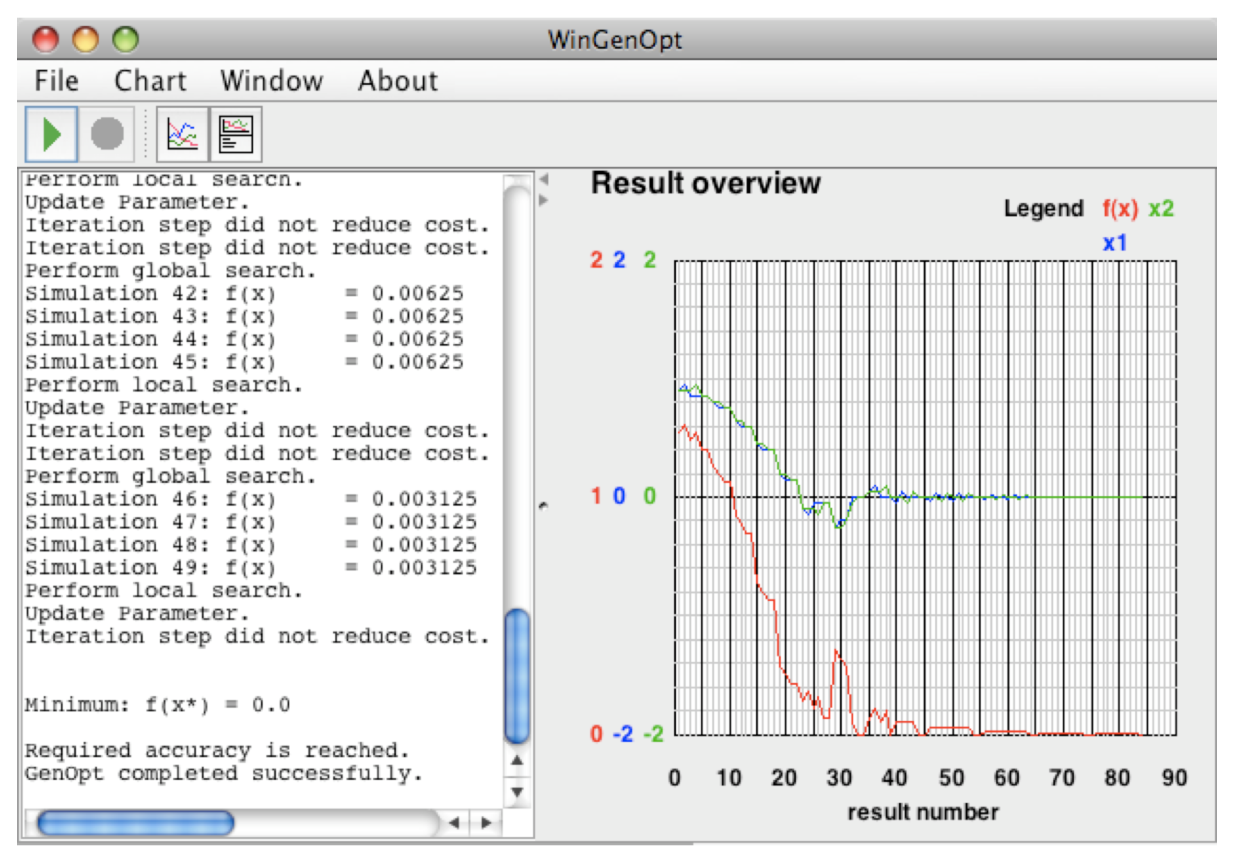
\epsfig{file=img/wingenopt.eps, width=\headwidth}
\caption{Output of GenOpt on Mac OS X for the example file in the directory {\tt example/quad/GPSHookeJeeves}.}
\label{fig:wingenoptGPSHJ}
\end{figure}

\chapter{Setting Up an Optimization Problem}
\label{sec:SetUpOptPro}
We will now discuss how to set up an optimization problem.\\


First, define a cost function.
The cost function is the function that needs to be minimized.
It must be evaluated by an external simulation program
that satisfies the requirements listed on page~\pageref{lis:simProIntReq}.
To maximize a cost function, 
change the sign of the cost function to turn the maximization problem
into a minimization problem.

Next,
specify possible constraints on the independent variables
or on dependent variables 
(dependent variables are values that are computed in the simulation program).
To do so,
use the default scheme for box constraints on the 
independent variables or
add penalty or barrier functions to the cost function
as described in Chapter~\ref{cha:conGen}.

Next, make sure that the simulation program
writes the cost function value to the simulation output file.
\emph{It is important that the cost function value is written 
to the output file without truncating any digits} 
(see Section~\ref{sec:hanOfNulSpaGen}).
For example, if the cost function is computed by a Fortran program
in double precision, 
it is recommended to use the \verb$E24.16$ format in the \text{write} statement.

In the simulation output file, the cost function value must be indicated by a
string that stands in front of the cost function value
(see page~\pageref{ite:simFilOut}).

Then, specify the files described in Section~\ref{sec:FilSpe} and, if required,
implement pre- and post-processing, as described in Section~\ref{par:posPro}.\\

% -------------------------------------------------------------------
\section{File Specification}
\label{sec:FilSpe}
This section defines the file syntax for GenOpt.
The directory \url{example} of the GenOpt installation contains several examples.\\

The following notation will be used to explain the syntax:
\begin{enumerate}
\item Text that is part of the file is written in \verb$fixed width fonts$.
\item \verb$|$ stands for possible entries. Only one of the entries that are separated by \verb$|$ is allowed.
\item \verb$[ ]$ indicates optional values.
\item The file syntax follows the Java convention. Hence,
\begin{enumerate}
\item \verb$//$ indicates a comment on a single line,
\item \verb$/*$ and \verb$*/$ enclose a comment,
\item the equal sign, \verb$=$, assigns values,
\item a statement has to be terminated by a semi-colon, \verb$;$,
\item curly braces, \verb${ }$, enclose a whole section of statements, and
\item the syntax is case sensitive.
\end{enumerate}
\end{enumerate}

\noindent The following basic types are used:\\[5mm]
\begin{tabular}{|l|l|} \hline
\verb$String$ & Any sequence of characters.\\ &
  If the sequence contains a blank character,\\ &
 it has to be enclosed in apostrophes (\verb$"$). \\
  &  If there are apostrophes within quoted text,\\ &
  they must be specified by a leading backslash (i.e., \verb$\"$). \\ &
 Similarly, a backslash must be preceded by another \\ &
 backslash (i.e., \verb$"c:\\go_prg"$).
\\ \hline
\verb$StringReference$  &  Any name of a variable that appears in the same section. \\ \hline
\verb$Integer$  &  Any integer value. \\ \hline
\verb$Double$  &  Any double value (including integer). \\ \hline
\verb$Boolean$  &  Either \verb$true$ or \verb$false$ \\ \hline
\end{tabular}
~\\


The syntax of the GenOpt files is structured into sections of parameters that belong to the same object. The sections have the form
\begin{lstlisting}
   ObjectKeyWord { Object }
\end{lstlisting}
where \verb$Object$ can either be another \verb$ObjectKeyWord$
or an assignment of the form
\begin{lstlisting}
   Parameter = Value ;
\end{lstlisting}

Some variables can be referenced. 
References have to be written in the form
\begin{lstlisting}
   Parameter = ObjectKeyWord1.ObjectKeyWord2.Value ;
\end{lstlisting}
where \verb$ObjectKeyWord1$ refers to the root of the object hierarchy as specified in the corresponding file.\\

% ---------------------------
\subsection{Initialization File}
\label{sec:IniFilSyn}
The initialization file specifies 
\begin{enumerate}
\item where the \emph{files} of the current optimization problems are located,
\item which simulation files the user likes to have saved for later inspection,
\item what additional strings have to be passed to the command that starts the simulation (such as the name of the simulation input file),
\item what number in the simulation output file is a cost function value,
\item whether and if so, how, the cost function value(s) have to be post-processed,
and
\item which simulation program is being used.
\end{enumerate}

The sections must be specified in the order shown below.
The order of the keywords in each section is arbitrary, as long as the numbers that follow some keywords (such as \texttt{File1}) are in increasing order.\\

\noindent The initialization file syntax is
\begin{lstlisting}
Simulation {
  Files {
    Template {
      File1 = String | StringReference;
    [ Path1 = String | StringReference; ]
      [ File2 = String | StringReference;
      [ Path2 = String | StringReference; ]
        [ ... ] ]
    }
    Input { // the number of input file must be equal to
            // the number of template files
      File1     = String | StringReference;
    [ Path1     = String | StringReference; ]
    [ SavePath1 = String | StringReference; ]
      [ File2     = String | StringReference;
      [ Path2     = String | StringReference; ]
      [ SavePath2 = String | StringReference; ]
        [ ... ] ]
    }
    Log {
    // The ``Log'' section has the same syntax as the ``Input'' section.
    }
    Output {
   // The ``Output'' section has the same syntax as the ``Input'' section.
    }
    Configuration {
      File1 = String | StringReference;
    [ Path1 = String | StringReference; ]
    }
  } // end of section Simulation.Files
  [CallParameter {
    [Prefix = String | StringReference;]
    [Suffix = String | StringReference;]
  }]
  [ObjectiveFunctionLocation {
    Name1       = String;
    Delimiter1  = String | StringReference;  |  Function1  = String;
    [FirstCharacterAt1 = Integer;]

    [ Name2       = String;
      Delimiter2  = String | StringReference;  |  Function2  = String;
      [FirstCharacterAt2 = Integer;]
    [ ... ] ]

  }]
} // end of section Simulation
Optimization {
  Files {
    Command {
      File1 = String | StringReference;
    [ Path1 = String | StringReference; ]
    }
  }
} // end of section Optimization
\end{lstlisting}
\pagebreak
\noindent The sections have the following meaning:
\begin{codedescription}
% -----------------------
\item[Simulation.Files.Template]
\label{sec:inpTemFil}
GenOpt writes the value of the independent variables
to the simulation input files.
To do so, GenOpt reads the simulation input \emph{template} files, replaces each occurrence of \verb$%variableName%$ by the numerical value of the corresponding variable, and the resulting file contents are written as the simulation input files. The string \verb$%variableName%$ refers to the name of the variable as specified by the entry \verb$Name$ in the optimization command file on page~\pageref{par:comFil}.\\

The independent variables can be written to several simulation input files if required.
To do so, specify as many \verb$Filei$ and \verb$Pathi$ assignments as necessary
(where \verb$i$ stands for a one-based counter of the file and path name).
Note that there must obviously be the same number of files and paths in the \verb$Input$ section that follows this section.\\

If there are multiple simulation input template files, each file will be written to the simulation input file whose keyword ends with the same number.\\ 

\noindent The following rules are imposed:
\begin{enumerate}
\item \label{rul:simTemVar} Each variable name specified in the optimization command file \emph{must} occur in at least one simulation input template file or in at least one function that is specified in the section \texttt{ObjectiveFunctionLocation} below.
\item \label{rul:simTemMul} Multiple occurrences of the same variable name are allowed in the same file and in the same function specification (as specified by the keyword \verb$Functioni$, \verb$i$ $= 1, 2, \ldots$).
\item If the value \verb$WriteStepNumber$ in the section \verb$OptimizationSettings$ of the optimization command file is set to \verb$true$, then rule \ref{rul:simTemVar} and \ref{rul:simTemMul} apply also to \verb$%stepNumber%$. If \verb$WriteStepNumber$ is set to \verb$false$, then \verb$%stepNumber%$ can occur, but it will 
be ignored.
\end{enumerate}

% -----------------------
\item[Simulation.Files.Input]
The simulation input file is generated by GenOpt based on the current parameter set and the corresponding simulation input \emph{template} file, as explained in the previous paragraph. Obviously, the number of simulation input files must be equal to the number of simulation input template files.\\

The section \verb$Input$ has an optional keyword, called \verb$SavePath$. If \verb$SavePath$ is specified, then the corresponding input file will after each simulation be copied into the directory specified by \verb$SavePath$. The copied file will have the same name, but with the simulation number added as prefix. 
% -----------------------
\item [Simulation.Files.Log]
GenOpt scans the simulation log file for error messages.
The optimization terminates if any of the strings specified by the variable \verb$ErrorMessage$ in the \verb$SimulationError$ section of the GenOpt configuration file is found. 
At least one simulation log file must be specified.\\

The section \verb$Log$ also has the optional keyword \verb$SavePath$.
It has the same functionality as explained in the previous section.

% -----------------------
\item[Simulation.Files.Output]
\label{ite:simFilOut}
GenOpt reads the cost function value from these files as described in 
the item {\tt Simulation.ObjectiveFunctionLocation} below.
The number of cost function values is arbitrary (but at least one must be specified). 
The optimization algorithms minimize the first cost function value.
The other values can be used for post-processing of the simulation output.
They will also be reported to the output files and the online chart.\\

\noindent GenOpt searches for the cost function value as follows:
\begin{enumerate}
\item 
After the first simulation, GenOpt searches for the first cost function value in the first output file
as described below in the description of
{\tt Simulation.ObjectiveFunctionLocation}.
If the first output file does not contain the first cost function value,
then GenOpt reads the second output file (if present) and so on until 
the last output file is read. 
If GenOpt cannot find the cost function value in any of the output files or function definitions, it will terminate with an error. The same procedure is repeated with the second cost function value, if present, until all cost function values have been found.
\item
In the following iterations, GenOpt will only read the file(s) where it found the cost function value(s) after the first simulation.
The files that did not contain a cost function value after the first simulation
will not be read anymore.
\end{enumerate}
This section also contains the optional keyword \verb$SavePath$.
If this keyword is specified, 
then GenOpt copies the output file.
This is particularly useful for doing parametric runs.
% -----------------------
\item[Simulation.Files.Configuration]
The entries in this section specify the simulation configuration file, which contains information that is related to the simulation program only, but not related to the optimization problem. The simulation configuration file is explained below.
% -----------------------
\item[Simulation.CallParameter]
Here, a prefix and suffix for the command that starts the simulation program can be added. With these entries, any additional information, 
such as the name of the weather file,
can be passed to the simulation program.
To do so, one has to refer to either of these entries in the argument of the keyword \verb$Command$ (see page~\pageref{key:com}).
% -----------------------
\item[Simulation.ObjectiveFunctionLocation]
\label{sec:objFunLoc}
This section specifies where the cost function values 
can be found in the simulation output files,
and possibly how these values have to be post-processed before they will be passed to the optimization algorithm.\\

To search for the cost function value, GenOpt reads the files
{\tt Simulation.Output.File1}, {\tt Simulation.Output.File2}, etc. one by one.
Each file is parsed starting at the last line and reading line-by-line towards 
the first line.
GenOpt assumes that the value that is written after the occurrence
of the string specified by \verb$Delimiteri$ (\verb$i$ $=1, 2, \ldots$)
is the cost function value.
Optionally, the entry \verb$FirstCharacterAti$ (\verb$i$ $=1, 2, \ldots$) can be used.
If \verb$FirstCharacterAti$ is greater than $0$, then delimiter \verb$Delimiteri$ must 
start at this position, otherwise it will be ignored.

For example, consider an output file that has the format
\begin{lstlisting}
5, 1.2345, 11
6, 12.345, 22 
\end{lstlisting}
Then, the entries
\begin{lstlisting}
Delimiter1  = "5,";
FirstCharacterAt1 = 0;
\end{lstlisting}
or, equivalently,
\begin{lstlisting}
Delimiter1  = "5,";
\end{lstlisting}
would cause GenOpt to return \verb$22$ as the objective function value, whereas 
the specification
\begin{lstlisting}
Delimiter1  = "5,";
FirstCharacterAt1 = 1;
\end{lstlisting}
would cause GenOpt to return \verb$1.2345$.\\

Alternatively to the entry \verb$Delimiteri$, an entry \verb$Functioni$ can be specified to define how the cost function values should be post-processed. 
If \verb$Functioni$ is specified, then \verb$FirstCharacterAti$ is ignored.
See page~\pageref{par:posPro} for an example that uses \verb$Functioni$.

For convenience, the section \verb$ObjectiveFunctionLocation$ can optionally be specified in the initialization file, but its specification is required in the configuration file. If this section is specified in both files, then the specification in the initialization file will be used.\\

Specifying the section \verb$ObjectiveFunctionLocation$ in the initialization file is of interest if a simulation program is used for different problems that require different values of this section. Then, the same (simulation program specific) configuration file can be used for all runs and the different settings can be specified in the (project dependent) initialization file rather than in the configuration file.

% -------------
\item[Optimization.Files.Command]
This section specifies where the optimization command file is located. This file contains the mathematical information of the optimization. See page~\pageref{par:comFil} for a description of this file.
\end{codedescription}
% -------------
\subsection{Configuration File}
The configuration file contains information related only to the simulation program used and not to the optimization problem. Hence, it has to be written only once for each simulation program and operating system.
We recommend to put this file in the directory \url{cfg} so that it can be used for different optimization projects. Some configuration files are provided with the GenOpt installation.\\

\pagebreak[4]
\noindent The syntax is specified by
\begin{lstlisting}
// Error messages of the simulation program.
SimulationError{
   ErrorMessage = String;
  [ErrorMessage = String;
  [ ... ] ]
}

// Number format for writing simulation input files.
IO{
   NumberFormat = Float | Double;
}

// Specifying how to start the simulation program.
SimulationStart{
   Command = String; 
   WriteInputFileExtension = Boolean;
}

// Specifying the location of the
// cost function value in the simulation output file
ObjectiveFunctionLocation{
    Name1       = String;
    Delimiter1  = String | StringReference;  |  Function1  = String;

    [ Name2       = String;
      Delimiter2  = String | StringReference;  |  Function2  = String;
    [ ... ] ]
}
\end{lstlisting}

\noindent The entries have the following meaning:
\begin{codedescription}

\item [SimulationError]
The error messages that might be written by the simulation program must be assigned to the keyword \verb$ErrorMessage$ so that GenOpt can check whether the simulation has completed successfully. At least one entry for \verb$ErrorMessage$ must be given.

\item[IO]
The keyword \verb$NumberFormat$ specifies in what format the independent parameters will be written to the simulation input file. The setting \verb$Double$ is recommended, unless the simulation program cannot read this number format.\\

\item[SimulationStart]
\label{key:com}
The keyword \verb$Command$ specifies what string must be used to start the simulation program.
It is important that this command waits until the simulation terminates 
(see the directory \texttt{cfg} for examples).
The value of the variable \verb$Command$ is treated in a special way: 
Any value of the optimization initialization file can be 
automatically copied into the value of \verb$Command$. 
To do so, surround the reference to the corresponding keyword with percent signs.
For example, a reference to the keyword 
\verb$Prefix$ of the initialization file looks like
\begin{lstlisting}
 %Simulation.CallParameter.Prefix%
\end{lstlisting}

By setting \verb$WriteInputFileExtension$ to \verb$false$, the value of the keyword \url{Simulation.Input.Filei} (where \verb$i$ stands for \verb$1$, \verb$2$, \verb$3$) is copied into \verb$Command$, and the file extension is removed.

\item[ObjectiveFunctionLocation]
Note that this section can also be specified in the initialization file.
The section in this file is ignored if this section is also specified in the 
configuration file.
See page~\pageref{sec:objFunLoc} for a description.
\end{codedescription}

\subsection{Command File}
\label{par:comFil}
The command file specifies optimization-related settings such as 
the independent parameters, 
the stopping criteria and the optimization algorithm being used.
The sequence of the entries in all sections of the command file is arbitrary.\\

There are two different types of independent parameters, 
{\em continuous parameters} and {\em discrete parameters}. 
Continuous parameters can take on any values, 
possibly constrained by a minimum and maximum value.
Discrete parameters can take on only user-specified discrete values,
to be specified in this file.\\

Some algorithms require all parameters to be continuous, 
or all parameters to be discrete, or allow both continuous and discrete parameters. 
Please refer to the algorithm section on page~\pageref{sec:algImp}-\pageref{sec:algImpEnd}.\\

%-----------------------------------
\subsubsection{Specification of a Continuous Parameter}
\label{subsubsec:SpeConPar}
\noindent The structure for a continuous parameter is
\begin{lstlisting}
// Settings for a continuous parameter
Parameter{
   Name = String;
   Ini  = Double;
   Step = Double;
   [ Min  = Double | SMALL; ]
   [ Max  = Double | BIG; ]
   [ Type = CONTINUOUS; ]
}
\end{lstlisting}
The entries are:
\begin{codedescription}
\item [Name] 
The name of the independent variable.
GenOpt searches the simulation input template files for 
this string -- surrounded by percent signs -- and replaces each occurrence 
by its numerical value before it writes the simulation input files.
\item [Ini] 
Initial value of the parameter.
\item [Step] 
\label{ite:parStep}
Step size of the parameter.
How this variable is used depends on the optimization algorithm being used.
See the optimization algorithm descriptions for details.
\item [Min] 
Lower bound of the parameter.
If the keyword is omitted or set to \verb$SMALL$, the parameter has no lower bound.
\item [Max] 
Upper bound of the parameter. If the keyword is omitted or set to \verb$BIG$, the parameter has no upper bound.
\item [Type] 
Optional keyword that specifies that this parameter is continuous. By default, if neither \verb$Type$ nor \verb$Values$ (see below) are specified, then the parameter is considered to be continuous and the \verb$Parameter$ section must have the above format.
\end{codedescription}

%-----------------------------------
\subsubsection{Specification of a Discrete Parameter}
\label{subsubsec:SpeDisPar}
For discrete parameters you need to 
specify the set of admissible values.
Alternatively, if a parameter is spaced either 
linearly or logarithmically, 
specify the minimum and maximum value of the parameter and the number of intervals.\\

First, we list the entry for the case of specifying the set of admissible values:
\begin{lstlisting}
// Settings for a discrete parameter
Parameter{
   Name   = String;
   Ini    = Integer;
   Values = String;
 [ Type   = SET; ]
}
\end{lstlisting}
The entries are:
\begin{codedescription}
\item [Name] {\it As for the continuous parameter above.}

\item [Ini] $1$-based index of the initial value. For example, if \verb$Values$ specifies three admissible values, then \verb$Ini$ can be either \verb$1$, \verb$2$, or \verb$3$.

\item [Values] Set of admissible values. The entry must be of the form\\
\verb$  Values = "value1, value2, value3";$\\
i.e., the values are separated by a comma,
and the list is enclosed in apostrophes (\verb$"$). 
For \verb$value1$, \verb$value2$, etc., numbers and strings are allowed.\\
If all entries of \verb$Values$ are numbers, then the result reports contain the actual values of this entry. Otherwise, the result reports contain the index of this value, i.e., \verb$1$ corresponds to \verb$value1$, \verb$2$ corresponds to \verb$value2$, etc.

\item [Type] Optional keyword that specifies that this parameter is discrete. By default, if the entry \verb$Values$ is specified, a parameter is considered to be discrete, and the \verb$Parameter$ section must have the above format.
\end{codedescription}
%-----------------------------------
\vspace{2\baselineskip}
To obtain linear or logarithmic spacing between a minimum and maximum value,
the \texttt{Parameter} section can be specified as
\begin{lstlisting}
// Settings for a discrete parameter, linearly or logarithmically spaced
Parameter{
   Name = String;
   Ini  = Integer;
   Type = SET;
   Min  = Double;
   Max  = Double;
   Step = Integer;
}
\end{lstlisting}
\begin{codedescription}
  \item [Name] {\it As for the continuous parameter above.}

\item [Ini] $1$-based index of the initial value. For example, if \verb$Step$ is set to $+2$ or to $-2$, then \verb$Ini$ can be set to any integer between $1$ and $3$.

\item [Type] This variable must be equal to \verb$SET$.

\item [Min] Minimum value of the spacing.

\item [Max] Maximum value of the spacing.

\item [Step] Number of intervals. If $\text{\texttt{Step}} < 0$, then the spacing is logarithmic, otherwise it is linear. Set $\text{\texttt{Step}} = 0$ to keep the parameter always fixed on its minimum value.
\end{codedescription}
The linear or logarithmic spacing is computed using \eqref{subeq:AlgParSpa} on page~\pageref{subeq:AlgParSpa}.\\

%-----------------------------------

\subsubsection{Specification of Input Function Objects}
\label{subsubsec:InpFunObj}
The specification of input function objects in optional.
If any input function object is specified, then its name
must appear either in another input function object, in
a simulation input template file, or in
an output function object.
Otherwise, GenOpt terminates with an error message.
See Section~\ref{par:posPro} on page~\pageref{par:posPro} for an explanation of input and output function
objects.\\

The syntax for input function objects is
\begin{alltt}
// Input function objects entry
Function\{
   Name     = String;
   Function = String;
\}
\end{alltt}
The entries are
\begin{codedescription}
\item [Name] A unique name that is not used for any other input function object
and for any other independent parameter.
\item [Function] A function object (see Section~\ref{par:posPro} on page~\pageref{par:posPro}).
The string must be enclosed by apostrophes (\texttt{"}).
\end{codedescription}

%-----------------------------------

\subsubsection{Structure of the Command File}
\noindent Using above structures of the \verb$Parameter$ section, the command file has the structure
\begin{alltt}
// Settings of the independent parameters
Vary\{
   // Parameter entry
    {\it List any of the} \texttt{Parameter} {\it sections as described}
    {\it in the Sections \ref{par:comFil}.\ref{subsubsec:SpeConPar} and \ref{par:comFil}.\ref{subsubsec:SpeDisPar}.}

   // Input function object
    {\it List any of the} \texttt{Function} {\it sections as described}
    {\it in the Section \ref{par:comFil}.\ref{subsubsec:InpFunObj}.}
\}

// General settings for the optimization process
OptimizationSettings\{
   MaxIte           = Integer;
   WriteStepNumber  = Boolean;
 [ MaxEqualResults  = Integer; ]
 [ UnitsOfExecution = Integer; ]
\}

// Specification of the optimization algorithm
Algorithm\{
   Main = String;
   ... // any other entries that are required
       // by the optimization algorithm
\}
\end{alltt}
The different sections are:
\begin{codedescription}

\item [Vary] This section contains the definition of the independent parameter
and the input function objects.
See Sections~\ref{par:comFil}.\ref{subsubsec:SpeConPar}, \ref{par:comFil}.\ref{subsubsec:SpeDisPar},
and \ref{par:comFil}.\ref{subsubsec:InpFunObj} for possible entries.

\item[OptimizationSettings] This section specifies general settings of the optimization. \verb$MaxIte$ is the maximum number of iterations.
After \verb$MaxIte$ main iterations,
GenOpt terminates with an error message.\\
\verb$WriteStepNumber$ specifies whether the current step 
of the optimization has to be written to the simulation input file or to a function object.
The step number can be used to calculate a penalty or barrier function
(see Section~\ref{sec:conDepVarGen} on page~\pageref{sec:conDepVarGen}).\\
The optional parameter \verb$MaxEqualResults$ specifies how many times 
the cost function value can be equal to a value that has previously been obtained 
before GenOpt terminates. 
This setting is used to terminate GenOpt if the cost function value
is constant for several iterates (see Section~\ref{sec:hanOfNulSpaGen}).
The default value of \verb$MaxEqualResults$ is $5$.\\
The optional parameter \verb$UnitsOfExecution$ specifies the maximum number of simulations
that may run in parallel. If this parameter is not specified or set to zero, then its value is set to
the number of processors of the computer that runs GenOpt. In general, this parameter need
not be specified.

\item[Algorithm] The setting of \verb$Main$ specifies which algorithm is invoked for doing the optimization.
Its value has to be equal to the class name that contains the algorithm. Note that additional parameters might be required depending on the algorithm used (see Section~\ref{sec:algImp} for the implemented algorithms).
\end{codedescription}

% =========================================================
\subsection{Log File}
GenOpt writes a log file to the directory that contains the initialization file. The name of the log file is \url{GenOpt.log}.

The GenOpt log file contains general information about the optimization process. It also contains warnings and errors that occur during the optimization.\\

% =========================================================
\subsection{Output Files}
In addition to \url{GenOpt.log}, GenOpt writes two output files to the directory
where the optimization command file is located.
(The location of the optimization command file is defined by 
the variable \url{Optimization.Files.Command.Path1} in the optimization initialization file.)

The iterations are written to the output files 
\url{OutputListingMain.txt} 
and \url{OutputListingAll.txt}.
The file \url{OutputListingMain.txt} contains only the main iteration steps,
whereas \url{OutputListingAll.txt} contains all iteration steps.\\

Each time the method \url{genopt.algorithm.Optimizer.report()}
is called from the optimization algorithm, 
the current trial is reported in either one of the files.

% =========================================================
\section{Resolving Directory Names for Parallel Computing}
To allow doing simulations using parallel computing, GenOpt will create a
temporary directory for each simulation.
This avoids different simulations writing to the
same output or log files simultaneously. 
The simulations will be done in subdirectories of the 
directory that contains the optimization initialization file. 

To explain which directories are created by GenOpt, suppose that GenOpt's 
optimization initialization file is stored in the directory {\tt /data/optMacOSX.ini}.
(For Windows, simply replace {\tt /data} with {\tt C:$\backslash$data} and replace all forwardslashes with
backslashes.) Suppose that GenOpt's initialization file states that the simulation input file
is {\tt /data/input/in.txt}, the simulation log file is {\tt /data/log.txt},
and the simulation output file is {\tt /data/output/out.txt}. 
Thus, in this example, the simulation will 
read its input from {\tt input/in.txt}, 
it will write its log messages to
{\tt log.txt}, and it will write its output
to {\tt output/out.txt}, where the directories {\tt input} and 
{\tt output} are subdirectories of the directory in which
the simulation was started.
Then, for the first simulation, GenOpt will proceed as follows:
\begin{enumerate}
\item It will create the simulation input file {\tt /data/tmp-genopt-run-1/input/in.txt} (including the temporary directory {\tt tmp-genopt-run-1/input}).
\item It will change the working directory for the simulation to the directory {\tt /data/tmp-genopt-run-1}.
Hence, if the simulation program writes to the current directory,
then it will write to {\tt /data/tmp-genopt-run-1}.
\item GenOpt will read {\tt /data/tmp-genopt-run-1/log.txt} to retrieve the simulation log messages.
\item If no error has been found in the log file, then 
GenOpt will read the simulation output file {\tt /data/tmp-genopt-run-1/output/out.txt}.
\item GenOpt will delete the directory {\tt /data/tmp-genopt-run-1} and all its subdirectories.
\end{enumerate}
For the second simulation, the same steps will be repeated, but the temporary directory will be
{\tt /data/tmp-genopt-run-2}.\\

To resolve the directory names, GenOpt uses the following rules. The rules are applied to 
the directories of the simulation input files, simulation log files and simulation output files.
They are also applied to the value of the keyword
{\tt Command} in the section {\tt SimulationStart} of the optimization configuration file.
\begin{enumerate}
\item \label{en:rulPat1} 
A period (``.'') is replaced by the path name of the optimization initialization file. 
\item
If the keywords {\tt Path1}, {\tt Path2} etc. are not specified in the optimization
initialization file, then they will be set to the directory of the optimization initialization file.
\item
For the simulation input, the simulation log and the simulation output files, 
the string {\tt tmp-genopt-run-\#}, where {\tt \#} is the number of the simulation,
will be inserted between the name of the optimization initialization file 
and the subdirectory name of the simulation input, log or output file.
\item
When resolving the file names, a path separator (``$\backslash$" on Windows or ``/'' on Mac OS X and Linux) will be appended if needed.
\end{enumerate}

These rules work for situations in which the simulation program uses the current
directory, or subdirectories of the current directory,
to read input and write output, provided that the optimization configuration file
is also in the directory that contains the simulation input files.\\

For the declaration of the {\tt Command} line in the GenOpt configuration file,
we recommend using the full directory name. For example, we recommend using
\begin{alltt}
 Command = "./simulate.sh    [linebreak added]
   %Simulation.Files.Log.Path1%/%Simulation.Files.Log.File1%";
\end{alltt}
instead of 
\begin{alltt}
 Command = "./simulate.sh ./%Simulation.Files.Log.File1%";
\end{alltt}
The first version ensures that the argument that is passed to {\tt simulate.sh} 
is the simulation log file in the working directory that is used by the current simulation. 
However, in the second version, because of rule \eqref{en:rulPat1} the simulation log file 
will be in the directory of GenOpt's configuration file, 
and thus different simulations may write to the same simulation log file 
simultaneously, causing unpredictable behavior.

% =========================================================
\section{Pre-Processing and Post-Processing}
\label{par:posPro}
Some simulation programs do not have the capability to pre-process the independent variables,
or to post-process values computed during the simulation.
For such situations, GenOpt's {\it input function objects} and {\it output function objects} can be used.

\subsubsection{Function Objects}
Function objects are formulas whose arguments can be the independent variables,
the keyword {\tt stepNumber}, and for post-processing,
the result of the simulation.\\

Following functions are implemented:\\[\baselineskip]
\noindent
\begin{tabular}[h]{l|l}
Function & Returns \\ \hline
\texttt{add(x0, x1)} & $x^0 + x^1$\\
\texttt{add(x0, x1, x2)} & $x^0 + x^1 + x^2$ \\
\texttt{subtract(x0, x1)} & $x^0 - x^1$\\
\texttt{multiply(x0, x1)} & $x^0 \, x^1$ \\
\texttt{multiply(x0, x1, x2)} & $x^0 \, x^1 \, x^2$\\
\texttt{divide(x0, x1)}                & $x^0 / x^1$  \\
\texttt{log10(x0)}                     & $\mathrm{log}_{10}(x^0)$
\end{tabular}\\[\baselineskip]
Furthermore, all functions that are defined in the class \texttt{java.lang.StrictMath} and whose arguments and return type are of type \texttt{double} can be accessed by typing their name (without the package and class name).\\

In addition, users can implement any other static method with arguments 
and return type \texttt{double} by adding the method to 
\texttt{genopt/algorithm/util/math/Fun.java}. 
The method must have the syntax
\begin{alltt}
  public static double {\it methodName}(double x0, double x1) \{
    double r;
    // {\it do any computations }
    return r; 
  \}
\end{alltt}
The number of arguments is arbitrary.

Next, compile the file after adding new methods and recreate the file
\texttt{genopt.jar}.
This can be done by changing from a console window to the directory
where the file \texttt{Makefile} is located, and then typing
\begin{alltt}
   make jar
\end{alltt}
provided that your computer has a make systems and a java compiler.
If your computer does not have a make system, you may be able to enter the following commands from a console window:
\begin{alltt}
  cd src
  javac -Xlint:unchecked LISTOFJAVAFILES
  jar cfm ../genopt.jar genopt/Manifest.txt [continues on next line]
          LISTOFJAVAFILES genopt/img/* ../legal.html
  cd ..
  jar -i genopt.jar 
\end{alltt}
where \texttt{LISTOFJAVAFILES} need to be replaced with all java files that are in the directory \texttt{src} and its subdirectories.
\\

Next, we present an example for pre-processing and afterwards an example for 
post-processing.

\subsubsection{Pre-Processing}
\begin{example}
{\em
Suppose we want to find the optimal window width and height.
Let {\tt w} and {\tt h} denote the window width and height, respectively.
Suppose we want the window height to be $1/2$ times the window width,
and the window width must be between $1$ and $2$ meters.
Then, we could specify in the command file the section
\begin{alltt}
Parameter\{
   Name =   w;
   Ini  = 1.5;     Step = 0.05;
   Min  =   1;     Max  =    2;
   Type = CONTINUOUS;
\}
Function\{
   Name =   h;     Function = "multiply( \%w\%, 0.5 )";
\}
\end{alltt}
Then, in the simulation input template files, GenOpt will replace all occurrences of
\texttt{\%w\%} by the window width and all occurences of \texttt{\%h\%} 
by $1/2$ times the numerical value of \texttt{\%w\%}.
}
\rbox
\label{ex:preProc}
\end{example}

GenOpt does not report values that are computed by input functions.
To report such values, a user needs to specify them in the section 
\texttt{ObjectiveFunctionLocation}, as shown in Example~\ref{ex:postProc} below.

\subsubsection{Post-Processing}
\begin{example}
{\em
Suppose we want to minimize the sum of annual heating and cooling energy consumption, 
which we will call \emph{total energy}. 
Some simulation programs cannot add different output variables.
For example, EnergyPlus~\cite{Crawley2001:1}
writes the heating and cooling energy consumption separately 
to the output file. 
In order to optimize the total energy, 
the simulation output must be post-processed.\\

To post-process the simulation results in GenOpt, we can proceed as follows:\\
Suppose the cost function delimiter (see Section~\ref{sec:IniFilSyn}) 
for the heating and cooling energy are, respectively, 
\texttt{Eheat=} and \texttt{Ecool=}.
In addition, suppose we want to report the value of the variable \texttt{h} that has been 
computed by the input function object in Example~\ref{ex:preProc}.
 

Then, in the optimization initialization file 
(see Section~\ref{sec:IniFilSyn}) we can specify the section
\begin{alltt}
  ObjectiveFunctionLocation\{
     Name1 = E_tot;  Function1 = "add( \%E_heat\%, \%E_cool\% )";
     Name2 = E_heat; Delimiter2 = "Eheat=";  
     Name3 = E_cool; Delimiter3 = "Ecool=";  
     Name4 = height; Function4  = \%h\%; 
  \}
\end{alltt}
This specification causes GenOpt to 
(i) substitute the value of \texttt{h} in \texttt{Function4}, 
(ii) read from the simulation output file(s) the numbers that occur after the 
strings \texttt{Eheat=} and \texttt{Ecool=}, 
(iii) substitute these numbers into the function
\texttt{add( \%E\_heat\%, \%E\_cool\% )}, 
(iv) evaluate the functions \texttt{Function1} and 
\texttt{Function4},
and (v) minimize the sum of heating and cooling energy.
}
\rbox
\label{ex:postProc}
\end{example}

As arguments of the function defined above, we can use any name of an 
independent variable, of an input function object,
or the keyword \texttt{\%stepNumber\%}.\\

% =========================================================
\section{Truncation of Digits of the Cost Function Value}
\label{sec:hanOfNulSpaGen}

\begin{figure}[ht!]
  \centering
  \resizebox{\textwidth}{!}{%
    {\psset{xunit=3, yunit=15, arrowscale=2}
\begin{pspicture}(-2.2, -0.22)(2, 0.2)%
%\psgrid[subgriddiv=0, xunit=1, yunit=1, gridlabels=0](-2.3, -0.3)(2, 0.3)
\fileplot[plotstyle=line, linecolor=black, linewidth=0.5pt]{img/truncation1.dat}%
\fileplot[plotstyle=line, linecolor=red, linewidth=1pt]{img/truncation2.dat}%
\psline{->}(-2.2,0)(1.9,0)
\psline{->}(0,-0.22)(0,0.2)
\uput[-90](1.85,-1ex){$x$}
\uput[180](0, 0.18){$f(x)$}
\multido{\n=-2+0.5}{8}{%
  \psline[linewidth=1.5pt]{-}(\n,-2pt)(\n,2pt)%
  \psline[linewidth=0.25pt]{-}(\n,-0.2)(\n,0.15)%
}
\rput(0,0){%
  \multido{\n=-2.0+0.5}{8}{%
    \uput[-45](\n, -1ex){$\n$}
  }
}
\multido{\n=-0.20+0.05}{8}{%
  \psline[linewidth=0.25pt]{-}(-2,\n)(1.5,\n)%
  \psline[linewidth=1.5pt]{-}(-2pt,\n)(2pt,\n)%
}
\multido{\n=-0.2+0.1}{4}{%
  \uput[120](-1ex,\n){$\n$}
}
\end{pspicture}
}
%
  }
  \caption{Function~\eqref{eq:exFunTruDig} with machine precision and
with truncated digits.
The upper line shows the cost function value with machine precision, and
the lower line shows the cost function value with only 
two digits beyond the decimal point.}
  \label{fig:truSigDig}
\end{figure}
For $x' \in \Re^n$ and $f \colon \Re^n \to \Re$, assume there exists a
scalar $\delta > 0$ such that $f(x') = f(x'')$ for all 
$x'' \in B(x', \delta)$, where 
$B(x', \delta) \triangleq \{ x'' \in \Re^n \ | \
\| x' - x'' \| < \delta \}$.
Obviously, in $B(x', \delta)$, an optimization algorithm can fail
because iterates in $B(x', \delta)$ contain no information about
descent directions outside of $B(x', \delta)$.
Furthermore, in absence of convexity of $f(\cdot)$, the optimality of
$x'$ cannot be ascertain in general.

Such situations can be generated if the simulation program
writes the cost function value to the output file 
with only a few digits.
Fig.~\ref{fig:truSigDig} illustrates that truncating digits can cause 
problems particularly in domains of $f(\cdot)$ where the slope of $f(\cdot)$
is flat.
In Fig.~\ref{fig:truSigDig}, we show the function
\begin{equation}
  f(x) \triangleq 0.1 \, x - 0.1 \, x^2 + 0.04 \, x^4.
\label{eq:exFunTruDig}
\end{equation}
The upper line is the exact value of $f(\cdot)$, and the lower line is 
the rounded value of $f(\cdot)$ such that it has only two digits 
beyond the decimal point.
If the optimization algorithm makes changes in $x$ in the size of $0.2$,
then it may fail for $0.25 < x < 1$, which is far from the minimum.
In this interval, no useful information about the descent of $f(\cdot)$ 
can be obtained.
Thus, the cost function must be written to the output file without truncating digits.\\

To detect such cases, the optimization algorithm can cause GenOpt to check 
whether a cost function values is equal to a previous cost function value.
If the same cost function value is obtained more than a user-specified number
of times, 
then GenOpt terminates with an error message. 
The maximum number of equal cost function values is specified 
by the parameter \texttt{MaxEqualResults} in the command file (see page \pageref{par:comFil}).

GenOpt writes an information to the user interface and to the log file if
a cost function value is equal to a previous function value.

\chapter{Conclusions}
In system optimization 
it is not possible to apply a general optimization algorithm that works efficiently 
on all problems.
What algorithm should be used depends on the properties of the cost function,
such as the number of independent parameters,
the continuity of the cost function and its derivatives,
and the existence of local minima.
Thus a variety of optimization algorithms is needed.
To address this need, GenOpt has a library with different optimization algorithms
and an optimization algorithm interface that users can use to implement 
their own optimization algorithm if desired.\\

The fact that analytical properties of the cost function are unavailable 
for the class of optimization problems that GenOpt has been developed for
makes it possible to separate optimization and function evaluation.
Therefore, 
GenOpt has a simulation program interface that allows coupling any 
program that exchanges input and output using text files.
Hence,
users are not restricted to using a special program for evaluating the cost function. 
Rather, they can use the simulation program they are already using for their 
system design and development. 
Thus, the system can be optimized with little additional effort.\\

This open environment not only allows coupling any simulation program and 
implementing special purpose algorithms, 
but it also allows sharing algorithms among users.
This makes it possible to extend the algorithm library 
and thus extend GenOpt's applicability.\\

% =========================================================
\chapter{Acknowledgments}
The development of GenOpt was sponsored by grants from 
the Swiss Academy of Engineering Sciences (SATW), 
the Swiss National Energy Fund (NEFF) and 
the Swiss National Science Foundation (SNF) 
and is supported by the 
Assistant Secretary for Energy Efficiency
and Renewable Energy, 
Office of Building Technology Programs of the
U.S. Department of Energy, under Contract No.
DE-AC02-05CH11231.
I would like to thank these institutions for their generous support.

% =========================================================
\chapter{Legal}
\section{Copyright Notice}
GenOpt Copyright (c) \copyrightyears, The Regents of the University of California, through Lawrence Berkeley National Laboratory (subject to receipt of any required approvals from the U.S. Dept. of Energy).  All rights reserved.\\

If you have questions about your rights to use or distribute this software, please contact Berkeley Lab's Technology Transfer Department at \url{TTD@lbl.gov}.\\

{\bf NOTICE.} This software was developed under partial funding from the U.S. Department of Energy.  As such, the U.S. Government has been granted for itself and others acting on its behalf a paid-up, nonexclusive, irrevocable, worldwide license in the Software to reproduce, prepare derivative works, and perform publicly and display publicly.  Beginning five (5) years after the date permission to assert copyright is obtained from the U.S. Department of Energy, and subject to any subsequent five (5) year renewals, the U.S. Government is granted for itself and others acting on its behalf a paid-up, nonexclusive, irrevocable, worldwide license in the Software to reproduce, prepare derivative works, distribute copies to the public, perform publicly and display publicly, and to permit others to do so.

\section{License agreement}
GenOpt Copyright (c) \copyrightyears, The Regents of the University of California, through Lawrence Berkeley National Laboratory (subject to receipt of any required approvals from the U.S. Dept. of Energy).  All rights reserved.\\

Redistribution and use in source and binary forms, with or without modification, are permitted provided that the following conditions are met:
\begin{enumerate}
\item
Redistributions of source code must retain the above copyright notice, this list of conditions and the following disclaimer.
\item
Redistributions in binary form must reproduce the above copyright notice, this list of conditions and the following disclaimer in the documentation and/or other materials provided with the distribution.
\item
Neither the name of the University of California, Lawrence Berkeley National Laboratory, U.S. Dept. of Energy nor the names of its contributors may be used to endorse or promote products derived from this software without specific prior written permission.
\end{enumerate}

THIS SOFTWARE IS PROVIDED BY THE COPYRIGHT HOLDERS AND CONTRIBUTORS "AS IS" AND ANY EXPRESS OR IMPLIED WARRANTIES, INCLUDING, BUT NOT LIMITED TO, THE IMPLIED WARRANTIES OF MERCHANTABILITY AND FITNESS FOR A PARTICULAR PURPOSE ARE DISCLAIMED. IN NO EVENT SHALL THE COPYRIGHT OWNER OR CONTRIBUTORS BE LIABLE FOR ANY DIRECT, INDIRECT, INCIDENTAL, SPECIAL, EXEMPLARY, OR CONSEQUENTIAL DAMAGES (INCLUDING, BUT NOT LIMITED TO, PROCUREMENT OF SUBSTITUTE GOODS OR SERVICES; LOSS OF USE, DATA, OR PROFITS; OR BUSINESS INTERRUPTION) HOWEVER CAUSED AND ON ANY THEORY OF LIABILITY, WHETHER IN CONTRACT, STRICT LIABILITY, OR TORT (INCLUDING NEGLIGENCE OR OTHERWISE) ARISING IN ANY WAY OUT OF THE USE OF THIS SOFTWARE, EVEN IF ADVISED OF THE POSSIBILITY OF SUCH DAMAGE.\\

You are under no obligation whatsoever to provide any bug fixes, patches, or upgrades to the features, functionality or performance of the source code ("Enhancements") to anyone; however, if you choose to make your Enhancements available either publicly, or directly to Lawrence Berkeley National Laboratory, without imposing a separate written license agreement for such Enhancements, then you hereby grant the following license: a  non-exclusive, royalty-free perpetual license to install, use, modify, prepare derivative works, incorporate into other computer software, distribute, and sublicense such enhancements or derivative works thereof, in binary and source code form.

\appendix

\chapter{Benchmark Tests}
This section lists the settings used in the benchmark tests 
on page~\pageref{sec:algSimBenTes}.\\

The settings in \texttt{OptimizationsSettings} and \texttt{Algorithm} 
are the same for all runs expect for \texttt{Accuracy},
which is listed in the result chart on page~\pageref{tab:nelMeaBenMarRes}.\\

\noindent The common settings were:
\begin{alltt}
OptimizationSettings\{
    MaxIte          = 1500;
    WriteStepNumber = false;
\}

Algorithm\{
   Main = NelderMeadONeill;
   Accuracy = {\rm{} see page \pageref{tab:nelMeaBenMarRes}};
   StepSizeFactor = 0.001;
   BlockRestartCheck = 5;
   ModifyStoppingCriterion  = {\rm{} see page \pageref{tab:nelMeaBenMarRes}};
\}
\end{alltt}
The benchmark functions and the \texttt{Parameter} settings in the \texttt{Vary} section are shown below.

\section{Rosenbrock}
\begin{figure}
\centering
\epsfig{file=img/fun_rosen.eps, bb=130 90 725 505, width=0.7\headwidth}
\caption{Rosenbrock function.}
\label{fig:funRosBro}
\end{figure}

The Rosenbrock function that is shown in Fig \ref{fig:funRosBro} is defined as
\begin{equation}
   f(x) \triangleq 100 \, \bigl(x^2 - (x^1)^2\bigr)^2 + (1 - x^1)^2,
\end{equation}
where $x \in \Re^2$.
The minimum is at $x^* = (1, \, 1)$, with $f(x^*) = 0$.\\

\pagebreak[3]
\noindent The section \texttt{Vary} of the optimization command file was set to
\begin{lstlisting}
Vary{
   Parameter{
      Name =   x1; Min = SMALL; 
      Ini  = -1.2; Max = BIG; 
      Step =    1;
      }
   Parameter{
      Name =   x2; Min = SMALL;
      Ini  =    1; Max = BIG;
      Step =    1;
      }
}
\end{lstlisting}
\section{Function 2D1}
\begin{figure}
\centering
\epsfig{file=img/fun_f2d1_con.eps, bb=75 110 615 505, width=0.5\headwidth}
\caption{Contour plot of $\frac{\partial d f(x)}{\partial x^1}=0$ and $\frac{\partial d f(x)}{\partial x^2}=0$, where $f(x)$ is as in (\ref{eq:defF2D1}).}
\label{fig:funTwoDOne}
\end{figure}

This function has only one minimum point.
The function is defined as
\begin{equation}
   f(x) \triangleq \sum_{i=1}^3 f^i(x),
  \label{eq:defF2D1}
\end{equation}
with
\begin{eqnarray}
  f^1(x) & \triangleq & \langle b, \, x \rangle + \frac{1}{2} \langle x, \, Q \, x \rangle, \quad b \triangleq 
\begin{pmatrix}  1 \\ 2 \end{pmatrix}, \quad
 Q \triangleq \begin{pmatrix} 10 & 6 \\ 6 & 8 \end{pmatrix},  \\
  f^2(x) & \triangleq & 100 \, \arctan \bigl( (2-x^1)^2 + (2 - x^2 )^2 \bigr), \\
   f^3(x) & \triangleq & 50 \, \arctan \bigl( (0.5 + x^1)^2 + (0.5 + x^2)^2   \bigr),
\end{eqnarray}
where $x \in \Re^2$.
The function has a minimum at $x^* = (1.855340, \, 1.868832)$,
with $f(x^*) = -12.681271$.
It has two regions where the gradient is very small (see Fig. \ref{fig:funTwoDOne}).\\

\pagebreak[4]
\noindent The section \texttt{Vary} of the optimization command file is
\begin{lstlisting}
Vary{
   Parameter{
      Name = x0; Min = SMALL;
      Ini  = -3; Max = BIG;
      Step = 0.1;
   }
   Parameter{
      Name =  x1; Min = SMALL;
      Ini  =  -3; Max = BIG;
      Step = 0.1;
   }
}
\end{lstlisting}

\section{Function Quad}

The function ``Quad'' is defined as
\begin{equation}
   f(x) \triangleq \langle b, \, x \rangle + \frac{1}{2} \langle x, \, M \, x \rangle,
\end{equation}
where $b, x \in \Re^{10}$, $M \in \Re^{10 \times 10}$, and
\begin{equation}
   b \triangleq (10, \, 10, \, \ldots \, , \, 10 )^T.
\end{equation}
This function is used in the benchmark test with two different positive definite matrices $M$.
In one test case, $M$ is the identity matrix $I$ 
and in the other test case $M$ is a matrix, called $Q$, 
with a large range of eigenvalues. The matrix $Q$ has elements~\\[\baselineskip]
\begin{tabular}{*{10}{>{\tiny$} r <{$}} }
579.7818 & -227.6855 & 49.2126 & -60.3045 & -152.4101 & -207.2424 & 8.0917 & 33.6562 & 204.1312 & -3.7129 \\
-227.6855 & 236.2505 & -16.7689 & -40.3592 & 179.8471 & 80.0880 & -64.8326 & 15.2262 & -92.2572 & 40.7367 \\
49.2126 & -16.7689 & 84.1037 & -71.0547 & 20.4327 & 5.1911 & -58.7067 & -36.1088 & -62.7296 & 7.3676 \\
-60.3045 & -40.3592 & -71.0547 & 170.3128 & -140.0148 & 8.9436 & 26.7365 & 125.8567 & 62.3607 & -21.9523 \\
-152.4101 & 179.8471 & 20.4327 & -140.0148 & 301.2494 & 45.5550 & -31.3547 & -95.8025 & -164.7464 & 40.1319 \\
-207.2424 & 80.0880 & 5.1911 & 8.9436 & 45.5550 & 178.5194 & 22.9953 & -39.6349 & -88.1826 & -29.1089 \\
8.0917 & -64.8326 & -58.7067 & 26.7365 & -31.3547 & 22.9953 & 124.4208 & -43.5141 & 75.5865 & -32.2344 \\
33.6562 & 15.2262 & -36.1088 & 125.8567 & -95.8025 & -39.6349 & -43.5141 & 261.7592 & 86.8136 & 22.9873 \\
204.1312 & -92.2572 & -62.7296 & 62.3607 & -164.7464 & -88.1826 & 75.5865 & 86.8136 & 265.3525 & -1.6500 \\
-3.7129 & 40.7367 & 7.3676 & -21.9523 & 40.1319 & -29.1089 & -32.2344 & 22.9873 & -1.6500 & 49.2499
\end{tabular}
\\[5mm]
The eigenvalues of $Q$ are in the range of $1$ to $1000$.\\

The functions have minimum points $x^*$ at\\

\begin{tabular}{ >{$} l <{$}  >{$} r <{$} >{$} r <{$} }
\multicolumn{1}{r}{\text{Matrix} M:} & \multicolumn{1}{c}{I}   & \multicolumn{1}{c}{Q} \\ \hline
x^{*^0}  &  -10  &  -2235.1810 \\
x^{*^1}  &  -10  &  -1102.4510 \\
x^{*^2}  &  -10  &  790.6100 \\
x^{*^3}  &  -10  &  -605.2480 \\
x^{*^4}  &  -10  &  -28.8760 \\
x^{*^5}  &  -10  &  228.7640 \\
x^{*^6}  &  -10  &  -271.8830 \\
x^{*^7}  &  -10  &  -3312.3890 \\
x^{*^8}  &  -10  &  -2846.7870 \\
x^{*^9}  &  -10  &  -718.1490 \\ 
f(x^*)  &  -500  &  0 \\ \hline
\end{tabular}
\\[10mm]
Both test functions have been optimized with the same parameter settings.
The settings for the parameters \texttt{x0} to \texttt{x9} are all the same,
and given by
\begin{lstlisting}
Vary{
   Parameter{
      Name = x0; Min = SMALL;
      Ini  =  0; Max = BIG;
      Step =  1;
   }
}
\end{lstlisting}






\bibliographystyle{alpha}
\bibliography{xbib}
\end{document}
